\documentclass[11pt]{article}

% ---- Layout ----
\usepackage[margin=1in]{geometry}
\usepackage{setspace}
\usepackage{lmodern}
\usepackage[T1]{fontenc}
\usepackage[utf8]{inputenc}

% ---- Math ----
\usepackage{amsmath, amssymb}

% ---- Tables and Figures ----
\usepackage{graphicx}
\usepackage{booktabs}
\usepackage{float}
\usepackage{threeparttable}
\usepackage{tabularx}
\usepackage{multirow}
\usepackage{siunitx}
\usepackage[font=small, labelfont=bf]{caption}

% ---- Lists and Formatting ----
\usepackage{enumitem}
\usepackage{titlesec}

% ---- Diagrams ----
\usepackage{tikz}

% ---- Bibliography ----
\usepackage[style=apa, backend=biber]{biblatex}
\DeclareLanguageMapping{american}{american-apa}
\addbibresource{references.bib}

% ---- Colors ----
\usepackage{xcolor}

% ---- Hyperlinks (load last among standard packages) ----
\usepackage{hyperref}
\hypersetup{
  colorlinks=true,
  linkcolor=black,
  citecolor=black,
  urlcolor=black
}

% ---- Working Paper Overlay ----
\usepackage{eso-pic}

% ---- Paths ----
% Figures: paper/figures/ for paper-ready, ../output/figures/ for analysis output
\graphicspath{{figures/}}
% Tables: \input with relative path from paper/
% e.g., \input{tables/tab_main_results}

% ---- Standard paragraph formatting ----
\setlength{\parindent}{1.5em}
\setlength{\parskip}{0pt}

% ---- Appendix figure/table numbering ----
\newcommand{\appendixnumbering}{%
  \setcounter{table}{0}%
  \renewcommand{\thetable}{A\arabic{table}}%
  \setcounter{figure}{0}%
  \renewcommand{\thefigure}{A\arabic{figure}}%
}

% ------------------------------------------------------------
% WORKING PAPER HEADER
% ------------------------------------------------------------
\newcommand{\workingpaperheader}{%
\AddToShipoutPictureFG*{%
  \AtPageUpperLeft{%
    \hspace*{0pt}%
    \raisebox{-1.10in}{%
      \parbox{\paperwidth}{%
        \centering
        {\small\bfseries WORKING PAPER}\\[-0.25em]
        {\small Draft: April 2026}\\[0.05em]
        \rule{0.75\paperwidth}{0.4pt}%
      }%
    }%
  }%
}%
}

% ---- Title ----
\title{\LARGE\bfseries Merit Aid, Sorting, and Institutional Access:%
  \\[0.3em] Evidence from Tennessee's HOPE Scholarship%
  \thanks{We are grateful to
  \href{mailto:dg3342@columbia.edu}{Daniel Garcia},
  \href{mailto:fam2175@columbia.edu}{Francine Montecinos Puente}, and
  \href{https://sites.google.com/view/seyhan-erden/home}{Seyhan Erden}
  (Columbia University);
  \href{https://www.hridaykarnani.com/}{Hriday Karnani}
  (Harvard University); and
  \href{mailto:as7596@columbia.edu}{Andrea Scalenghe}
  (MIT Sloan)
  for helpful discussions and comments. We also thank the Federal Reserve
  Bank of Cleveland and the Peer Review Board of the Economic Scholars
  Program. The views expressed herein are those of the authors and do not
  necessarily reflect the views of the Federal Reserve Bank of New York
  or Columbia University.}}

\author{%
  \vspace{-0.2em}\\
  {\large
  \href{mailto:bok2106@columbia.edu}{Balint Kidd} \quad
  \href{mailto:trs2169@columbia.edu}{Tommy Soltanian} \quad
  \href{mailto:tyler.sotomayor@columbia.edu}{Tyler Sotomayor} \quad
  \href{mailto:gu2145@columbia.edu}{Gabriel Uceda-Sosa}} \\[0.7em]
  {\large Columbia University} \\[0.7em]
  {\normalsize April 2026} \\[1.2em]
  {\small\color{blue}\href{https://www.tylersotomayor.com/merit}{Link to Most Current Version}}
}

\date{\vspace{-3em}}

% ============================================================
\begin{document}
% ============================================================

\workingpaperheader

\begingroup
\onehalfspacing
\maketitle

\vspace{1em}

\begin{abstract}
\noindent
Merit-based scholarship programs are widely viewed as regressive because
eligibility correlates with family income. We show that this conclusion
conflates individual attendance effects with institutional composition
effects---distinct estimands that can move in opposite directions when
students sort across multiple sectors. Using tax-linked data from
\textcite{chetty2020mobility}, we find that Tennessee's HOPE Scholarship
reshapes the full parental income distribution at public colleges: all
five income quintiles shift monotonically, with bottom-quintile share
rising and top-quintile share falling. Total enrollment is unchanged;
the shift reflects three-destination sorting in which lower-income
students enter from non-attendance while upper-income students exit to
out-of-state alternatives. A permutation test ($p = 0.037$ for parental
income rank, $p = 0.074$ for bottom-quintile share) and synthetic
control analysis confirm Tennessee as an outlier. Results are robust
across four heterogeneity-corrected estimators. Massachusetts' Adams
Scholarship independently produces a progressive shift of similar
magnitude under similar design parameters, while South Dakota's
high-threshold program produces the opposite pattern---as the model
predicts. A three-destination sorting framework reconciles these
progressive composition effects with the regressive attendance findings
of \textcite{dynarski2000hope} and identifies program design parameters
that determine sorting direction.
\end{abstract}

\vspace{1em}

\noindent \textbf{JEL Codes:} I23, I24, I28, H75, J24, C23

\vspace{0.25em}

\noindent \textbf{Keywords:} merit aid, college composition, sorting, HOPE Scholarship, difference-in-differences

\endgroup

\doublespacing
\newpage

\tableofcontents
\newpage

% ============================================================
%  BODY
% ============================================================

% ============================================================
%  SECTION 1: INTRODUCTION
% ============================================================

\section{Introduction}

\textcite{dynarski2000hope} showed that Georgia's HOPE Scholarship
widened the gap in college attendance between higher- and lower-income
students. The finding crystallized a distributional critique of merit
aid: because eligibility is conditioned on academic achievement, which
correlates with family income, broad-based merit programs
disproportionately subsidize students who would attend college regardless
\parencite{dynarski2004merit, jones2022merit}. This view now dominates
the policy debate.

A systematic review of 71 quasi-experimental studies finds that
merit-based grants rarely improve outcomes for disadvantaged students and
can increase inequality \parencite{herbaut2020works}. We document an
exception.

Using tax-linked income data from \textcite{chetty2020mobility}, we
estimate how Tennessee's HOPE Scholarship reshaped the full parental
income distribution at public colleges. The results are the opposite of
what the conventional view predicts: following HOPE implementation,
public colleges experienced a \emph{progressive} compositional shift.
Bottom-quintile students gained share at public institutions, while
top-quintile students lost share. The effect is monotonic across all
five income quintiles---Q1 through Q3 gain, Q4 and Q5 lose---and every
coefficient is statistically significant. This monotonic gradient is the
paper's central empirical result.

Aggregate attendance effects and institutional composition effects are
distinct estimands that need not move in the same direction. In a
two-sector model---attend college or not---individual enrollment
responses fully determine institutional composition. But when students
choose among public, private, and out-of-state alternatives, the link
breaks: the \emph{aggregate} attendance gap can widen (because
higher-income students are more likely to qualify) while the
\emph{sector-specific} composition of public colleges simultaneously
improves (because the students who actually sort into the public sector
are drawn disproportionately from the bottom of the income
distribution).\footnote{This is a form of Simpson's paradox: the
aggregate relationship between merit aid and income composition reverses
sign when conditioned on enrollment sector. The aggregate effect reflects
who attends college; the composition effect reflects who attends
\emph{which} college.} The reconciliation depends on where displaced
students go. If top-quintile students exit to out-of-state or private
alternatives rather than entering public colleges, the public sector
becomes more progressive even as overall college-going becomes more
unequal. We formalize this insight in a three-destination sorting model
(public, private, out-of-state) and test its predictions directly.

Institutional composition matters independently of individual enrollment
decisions. The peer effects literature demonstrates that student body
composition shapes academic outcomes
\parencite{sacerdote2001peer}. \textcite{chetty2020mobility} show that
access to high-mobility institutions drives intergenerational economic
outcomes, establishing that who attends which institution has first-order
welfare consequences. If merit aid systematically alters the income
profile of public college cohorts, it reshapes the peer environment and
mobility prospects for all enrolled students---not only those on the
margin of attendance.

Four pieces of evidence are consistent with a sorting interpretation.
First, total enrollment at Tennessee public colleges is unchanged after
HOPE. The share shifts reflect real reallocation---11 additional
bottom-quintile students per cohort enter, 34 top-quintile students per
cohort exit---not a denominator artifact. Second, Tennessee private
colleges show no mirror image of the public-sector shift: the decline in
top-quintile representation at public colleges is not offset by gains at
Tennessee privates, consistent with out-of-state exit as the relevant
margin. Third, two-year and four-year institutions adjust through
different channels. Community colleges exhibit displacement
(top-quintile students replaced by bottom-quintile students, total seats
unchanged), while four-year colleges show expansion (enrollment grows,
composition shifts). Fourth, within-state comparisons restricted to
Tennessee institutions confirm that the composition change is specific
to the public sector.

These patterns may not be idiosyncratic to Tennessee. Our theoretical
framework proposes that program design and institutional context jointly
shape the direction of compositional sorting, through three parameters:
the eligibility threshold relative to the income distribution, the size
of the public-private subsidy differential, and interactions with
existing need-based aid. Georgia's
HOPE, which initially offset Pell Grant awards dollar-for-dollar and
imposed an income cap, eliminated the access margin for the
lowest-income families and muted the public-private subsidy
differential---conditions under which the model predicts regressive
sorting. Dynarski's findings for Georgia are consistent with this
prediction, as are the enrollment patterns documented by
\textcite{cornwell2006enrollment}. Tennessee's HOPE, which has no Pell
offset, no income cap, and a large public-private subsidy
differential, satisfies the conditions for progressive sorting. The same
framework explains both outcomes.

We test these predictions out of sample. Massachusetts' Adams
Scholarship \parencite{cohodes2014merit}, which shares Tennessee's
design features (moderate threshold, public-sector subsidy
concentration), independently produces a progressive shift of similar
magnitude ($+1.38$ pp for bottom-quintile share). South Dakota's
Opportunity Scholarship, which imposes a high ACT threshold and small
award, produces a strongly regressive shift---as the model predicts.
West Virginia's PROMISE, despite similar design parameters to
Tennessee, shows no compositional effect, highlighting that program
design is necessary but not sufficient: enrollment contraction at WV
public colleges overwhelmed any sorting dynamics.

We estimate treatment effects using \textcite{callaway2021difference} as
the primary estimator, with TWFE, \textcite{sun2021estimating}, and
\textcite{dechaisemartin2020two} for robustness. A bordering-state control
group passes pre-trend tests that the national comparison fails at
longer horizons. Results are stable across three treatment timing
definitions and two alternative control group specifications.
Under the relative-magnitude restriction of
\textcite{rambachan2023more}, the estimated effect survives violations
up to twice the magnitude observed in the pre-treatment period. Under
the stricter smoothness restriction, results are more fragile. We
interpret the evidence as credible but not definitive, and report all
sensitivity analyses transparently.

Our work connects three literatures. First, a large body of research
documents the enrollment effects of merit aid
\parencite{dynarski2000hope, dynarski2004merit, bruce2014jackpot,
cohodes2014merit, song2024hope, cummings2022race,
verzyl2023institutional}. This literature
focuses on individual enrollment decisions, not institutional
composition. Second, studies of policy-induced sorting show that
admissions and financing reforms can substantially reshape who attends
which institutions \parencite{bleemer2022affirmative,
card2005affirmative, hinrichs2012affirmative}. Third,
\textcite{chetty2020mobility} demonstrate that access to
high-mobility institutions shapes intergenerational economic outcomes,
establishing that institutional composition has first-order welfare
consequences. We bridge these literatures by documenting how merit aid is
associated with changes in the full income distribution across
institutional sectors.

This paper makes three contributions. First, we provide the first
evidence on how merit aid reshapes the \emph{full income distribution}
at public institutions, using tax-linked data that measures parental
income across all quintiles rather than relying on Pell eligibility as a
binary proxy. The monotonic quintile gradient---all five coefficients
significant and perfectly ordered---has not been documented in any prior
study of merit aid. Second, we develop a three-destination sorting
framework that reconciles the progressive institutional composition
effects we find with the regressive attendance effects documented by
\textcite{dynarski2000hope}, showing that the apparent contradiction
dissolves once student destinations are disaggregated. Third, we
propose that program design parameters---Pell interaction, subsidy
differential, threshold location---shape whether merit aid is associated
with progressive or regressive sorting, and test the framework across
four states: Tennessee and Massachusetts (progressive, as predicted),
South Dakota (regressive, as predicted), and West Virginia (null,
confounded by enrollment contraction).

The paper proceeds as follows. Section~\ref{sec:background} describes
the Tennessee HOPE Scholarship and the Georgia program that serves as
our theoretical comparison case. Section~\ref{sec:theory} presents the
three-destination sorting model and derives testable predictions.
Section~\ref{sec:data} describes the data.
Section~\ref{sec:empirical_strategy} discusses the empirical strategy.
Section~\ref{sec:results} presents results.
Section~\ref{sec:robustness} reports robustness checks.
Section~\ref{sec:discussion} discusses cross-state evidence from
Georgia, Massachusetts, South Dakota, and West Virginia.
Section~\ref{sec:conclusion} concludes.


% ============================================================
%  SECTION 2: INSTITUTIONAL BACKGROUND
% ============================================================

\section{Institutional Background}
\label{sec:background}

\subsection{Tennessee HOPE Scholarship}

Tennessee introduced the HOPE Scholarship in 2003, funded by proceeds
from the state education lottery \parencite{THEC2025}. The program provides tuition and fee
subsidies to Tennessee residents who graduate from an eligible high
school with a minimum 3.0 GPA or score at least 21 on the ACT (or 980
on the SAT). Recipients must maintain a 2.75 cumulative GPA after the
first semester to retain eligibility
\parencite{ness2008eligibility}.

The scholarship provides a fixed dollar award covering approximately
60--80\% of in-state tuition at public institutions governed by the
Tennessee Board of Regents (TBR) and the University of Tennessee system
(\$3,000 for freshmen and sophomores, scaling to \$6,000 for juniors and
seniors at four-year institutions during the study period). Students
attending eligible private institutions receive a smaller fixed amount
(\$3,000--\$4,000 per year), which covers a substantially lower share
of private tuition. This differential generosity creates a relative price advantage
for public colleges---the key mechanism in our theoretical framework.

Table~\ref{tab:hope_distribution} reports the distribution of HOPE
recipients across sectors for the first five entering cohorts
(2004--2008). Public institutions---TBR universities, TBR community
colleges, and UT campuses---account for approximately 83--85\% of
recipients in every year. Private colleges receive 15--17\%. This
concentration of aid in the public sector motivates our identification
strategy: we treat Tennessee public colleges as the primary recipients
of the HOPE demand shock.

\subsection{Prior Research on TN HOPE}

Several studies examine Tennessee's merit aid program. The closest
antecedent is \textcite{bruce2014jackpot}, who use a regression
discontinuity at the ACT score cutoff for HOPE eligibility.
\textcite{chakrabarti2022merit} study merit aid and student mobility
more broadly, documenting how scholarship programs interact with college
selectivity. \textcite{bruce2014jackpot} find that Tennessee HOPE had no
effect on overall enrollment among Pell-eligible students near the ACT
threshold, but reallocated them from two-year to four-year public
institutions ($-2.9$ percentage points at community colleges, $+2.4$ at
four-year publics). For non-white students, overall enrollment declined
by 2.6 percentage points.

Our analysis is complementary but asks a different question. Bruce and
Carruthers estimate the \emph{individual enrollment response} at the
eligibility margin: how does a student just above the ACT cutoff choose
differently from one just below? Their RD is local to the threshold and
identifies the effect for compliers at that margin. We estimate the
\emph{institutional composition effect} across the full income
distribution: how does the parental income profile of the entire student
body at public colleges change after HOPE? Our
difference-in-differences design captures the average treatment effect
across all treated cohorts, including students well above the
eligibility threshold for whom the RD has no power. The distinction
matters because the composition of public colleges depends on the
sorting behavior of students at all income levels, not only those at
the eligibility margin. Our quintile decomposition---showing that all
five quintiles shift monotonically---documents a pattern that no
threshold-local design can detect, since students in the top quintile
are almost all well above any reasonable ACT cutoff. Their finding that
lower-income marginal students upgrade from community colleges to
four-year institutions is consistent with our result that bottom-quintile
share rises and that two-year and four-year colleges adjust through
different channels.

\subsection{Timeline and Cohort Mapping}
\label{sec:background_timeline}

The Tennessee HOPE Scholarship was enacted in 2003. In the
\textcite{chetty2020mobility} data, cohorts are indexed by birth year,
and students are assigned to institutions attended between ages 19 and
22. The analysis window spans birth cohorts 1980--1991, corresponding
approximately to college entry years 1998--2009.
Table~\ref{tab:cohort_map} maps each birth cohort to its decision year,
college entry year, event time, and HOPE exposure status.

\paragraph{Decision timing vs.\ receipt timing.}

The mechanism studied in this paper is sorting across institutional
sectors---public, private, and out-of-state---driven by the relative
price change that HOPE creates. Sorting occurs \emph{before}
matriculation, when students choose where to apply and enroll. The
economically relevant treatment date is therefore the point at which
HOPE enters the student's decision environment, not the date on which
scholarship funds are first disbursed.

We define the decision year as birth cohort $+ 17$, corresponding to
the year in which the student is typically a high-school senior forming
a college choice set. Under this mapping, the 1986 birth cohort has
decision year 2003---the same year HOPE was enacted. These students were
mid-application cycle when the program was announced; some could adjust,
but many had already committed. The 1987 birth cohort has decision year
2004 and is the first group whose entire college search occurred with
HOPE already enacted, publicized, incorporated into school counseling,
and operational in the financial aid environment.

Our preferred treatment timing is therefore $t^* = 1987$: the first
cohort whose college choice set was formed under the fully known HOPE
regime. We designate the 1986 cohort as the omitted reference period
($k = -1$), absorbing any partial treatment of this transition cohort
into the baseline. The 1985 cohort received limited retroactive benefits
through a bridge provision, but made enrollment decisions before HOPE
existed. The 1984 cohort (entering college Fall 2002) is the last
cohort with no HOPE exposure of any kind.

We test robustness to $t^* \in \{1985, 1986, 1987\}$ in
Section~\ref{sec:robustness}. The static DiD estimate is insensitive to
this choice.

\paragraph{Analysis window.}

Under the preferred timing, the sample provides five pre-treatment
cohorts (1981--1985) and five post-treatment cohorts (1987--1991), with
1986 as the omitted reference period. Each cohort's composition is
measured independently: the outcome for cohort $t$ at college $c$
reflects the parental income distribution of students born in year $t$
who attended college $c$ between ages 19 and 22. The 1980 birth cohort
is dropped from the preferred specification because Tennessee's
1980-born cohort exhibits anomalously low bottom-quintile share that
normalizes by 1982, consistent with a data artifact rather than a
substantive pre-trend. Dropping this single cohort substantially
improves sensitivity to violations of parallel trends
(Section~\ref{sec:robustness}).

\begin{table}[H]
\centering
\begin{threeparttable}
\caption{Cohort Mapping: Birth Year, Decision Year, and HOPE Exposure}
\label{tab:cohort_map}
\begin{tabular}{cccclc}
\toprule
Birth Cohort & Decision Year & College Entry & Event Time ($k$) & HOPE Status \\
\midrule
1980 & 1997 & Fall 1998 & --- & No HOPE (dropped$^\dagger$) \\
1981 & 1998 & Fall 1999 & $-6$ & No HOPE \\
1982 & 1999 & Fall 2000 & $-5$ & No HOPE \\
1983 & 2000 & Fall 2001 & $-4$ & No HOPE \\
1984 & 2001 & Fall 2002 & $-3$ & No HOPE \\
1985 & 2002 & Fall 2003 & $-2$ & Bridge provision (partial)$^\ddagger$ \\
1986 & \textbf{2003} & Fall 2004 & $-1$ & Transition (ref.\ period) \\
\midrule
1987 & \textbf{2004} & Fall 2005 & $0$ & Full HOPE ($t^*$) \\
1988 & 2005 & Fall 2006 & $+1$ & Full HOPE \\
1989 & 2006 & Fall 2007 & $+2$ & Full HOPE \\
1990 & 2007 & Fall 2008 & $+3$ & Full HOPE \\
1991 & 2008 & Fall 2009 & $+4$ & Full HOPE \\
\bottomrule
\end{tabular}
\begin{tablenotes}[flushleft]
\footnotesize
\item \textit{Notes:} Decision year $=$ birth cohort $+ 17$ (high-school
  senior year). College entry is approximate (birth cohort $+$ 18).
  Students are assigned to institutions attended between ages 19 and 22
  in the \textcite{chetty2020mobility} data. HOPE was enacted in 2003
  (bolded). $^\dagger$The 1980 cohort is dropped from the preferred
  specification; see text. $^\ddagger$Bridge provision extended limited
  retroactive benefits to Fall 2003 entrants who met eligibility
  criteria; these students made enrollment decisions before HOPE existed.
  Event times shown relative to $t^* = 1987$.
\end{tablenotes}
\end{threeparttable}
\end{table}

\paragraph{Confounding policies.}

Several other policy changes coincided with HOPE's introduction, and we
consider whether any could produce the quintile gradient we document.

Tennessee's education lottery launched in 2003 and generated revenue
that funded both HOPE and Pre-K programs. The federal No Child Left
Behind Act (2002) altered K--12 accountability requirements nationwide.
Both policies affect treated and control states symmetrically and are
absorbed by cohort fixed effects.

Federal Pell Grant generosity increased during our analysis window:
the 2007 College Cost Reduction Act raised maximum awards, and the
2009 American Recovery and Reinvestment Act added temporary increases.
These expansions apply nationally, so any composition effects are
absorbed by cohort fixed effects in our DiD design. To the extent
that Pell expansions disproportionately benefit low-income students,
they would produce a level shift in bottom-quintile enrollment at all
public colleges, not the Tennessee-specific treatment effect our
interaction term identifies.

Tennessee's Board of Regents expanded community college access during
this period, including the Tennessee Technology Centers and dual
enrollment initiatives. These reforms could affect overall enrollment
levels but would not generate a monotonically ordered gradient across
all five income quintiles---a pattern that requires differential price
sensitivity by parental income, as our model predicts.

Tuition changes at neighboring states' public universities could
affect cross-state sorting. However, such changes would
disproportionately influence border-county colleges rather than
producing the statewide pattern we observe.

While we cannot rule out every potential confounder individually, the
quintile gradient provides a useful discriminating pattern: a generic
enrollment shock would affect quintile shares unevenly but would be
unlikely to produce five coefficients that are monotonically ordered
across all quintiles with no effect at private institutions.

\subsection{Georgia HOPE as a Comparison Case}
\label{sec:background_georgia}

Georgia's HOPE Scholarship (1993) is the canonical case in the merit aid
literature \parencite{dynarski2000hope, song2024hope} and our primary
theoretical comparison. Three design features
distinguish it from Tennessee's program in ways that matter for our
sorting framework.

First, from 1993 to 2000, Georgia HOPE awards were reduced
dollar-for-dollar by Pell Grant amounts. Students from the
lowest-income families received zero net benefit from HOPE for the
program's first seven years. \textcite{dynarski2000hope} documents the
consequence: Black students, who were disproportionately Pell-eligible,
showed no attendance gain, while white students gained 12.3 percentage
points. The Pell offset effectively eliminated the access margin for
the bottom of the income distribution.

Second, Georgia imposed an income cap (\$66,000, later \$100,000,
eliminated in 1995) during the program's early years. While the cap
was removed relatively quickly, its presence during the launch shaped
initial enrollment patterns.

Third, Georgia HOPE provided comparable awards to private colleges:
initially full tuition, later a fixed \$3,000 that covered a
meaningful share of private tuition at Georgia's price levels. This
smaller public-private subsidy differential muted the sector-switching
mechanism that drives compositional sorting in our model. \textcite{cornwell2006enrollment} confirm that four-year private enrollment in
Georgia \emph{rose} by 13.2\% after HOPE, and two-thirds of the
four-year enrollment gain reflected reduced out-of-state migration
rather than new college-goers.

We return to the GA-TN comparison in Section~\ref{sec:theory_georgia},
where we show that these design differences generate opposite
predictions from the same theoretical framework.

\subsection{Florida Bright Futures: A Tuition-Scaling Contrast}
\label{sec:background_florida}

Florida's Bright Futures Scholarship (1997) provides a structural
contrast to Tennessee's fixed-dollar design. Bright Futures operates
on a multi-tier system. The top tier (Florida Academic Scholars)
requires a 3.5 weighted GPA and 1270~SAT, covering 100\% of tuition.
The broad-coverage tier---Florida Medallion Scholars---requires only
a 3.0 weighted GPA and 970~SAT (old scale, approximately the 50th
percentile nationally) and covers 75\% of tuition at public
institutions. During our study period (1998--2009), approximately
30--35\% of Florida high school graduates received some tier of
Bright Futures.

Two features distinguish Bright Futures from Tennessee HOPE for the
income-shock analysis. First, the award is \emph{percentage-based}:
it covers a fixed share of tuition rather than a fixed dollar amount.
When tuition rises, the award rises proportionally. This means the
gap between the scholarship and total tuition cost does not widen
over time---the theoretical distinction formalized in
Proposition~\ref{prop:compensation}. Second, Bright Futures does not
require FAFSA filing for eligibility, removing a paperwork barrier
that may deter low-income families during periods of financial stress.

Because Bright Futures was already active throughout the Chetty panel
(the program predates the 1998 college entry of the earliest cohort),
we cannot estimate an adoption DiD for Florida. The shock-interaction
design (Section~\ref{sec:empirical_shock}) circumvents this limitation
by comparing how Florida colleges respond to income shocks relative
to non-merit states, without requiring a pre-program period.


% ============================================================
%  SECTION 3: THEORETICAL FRAMEWORK
% ============================================================

\section{Theoretical Framework}
\label{sec:theory}

We develop a simple model of college choice that generates testable
predictions about how merit aid reshapes the income composition of
public institutions. The key departure from standard two-sector models
is that we allow three destinations: in-state public college, in-state
private college, and an outside option (out-of-state enrollment or
non-attendance).

\subsection{Setup}

Consider a population of families indexed by income $y_i$ and student
ability $a_i$, where $y_i$ and $a_i$ are positively correlated. Each
family chooses among three options: a public college ($C_P$), a private
college ($C_R$), or no college ($0$). The indirect utility of family
$i$ from option $j \in \{P, R, 0\}$ is
\begin{equation}
  V_{ij} = q_j - \frac{C_j}{y_i} + \varepsilon_{ij},
\end{equation}
where $q_j$ is the quality of institution $j$, $C_j$ is the sticker
price, and $\varepsilon_{ij}$ captures idiosyncratic preferences. We
normalize $q_0 = C_0 = 0$. Assume $q_R > q_P > 0$ and $C_R > C_P > 0$:
private colleges are both higher quality and more expensive.

\subsection{Merit Scholarship Introduction}

A state merit scholarship of amount $S > 0$ reduces the effective price
of the public college for students with ability above a threshold
$\tau$:
\begin{equation}
  C_P^{\text{eff}}(a_i) =
  \begin{cases}
    C_P - S & \text{if } a_i \geq \tau, \\
    C_P     & \text{if } a_i < \tau.
  \end{cases}
\end{equation}

Without the scholarship, families sort across options by income. Define
the no-college/public boundary as $\underline{y}$, where $V_{iP} =
V_{i0}$, and the public/private boundary as $\overline{y}$, where
$V_{iP} = V_{iR}$. In the absence of idiosyncratic preferences:
\begin{equation}
  \underline{y} = \frac{C_P}{q_P}, \qquad
  \overline{y} = \frac{C_R - C_P}{q_R - q_P}.
\end{equation}
Families with $y_i < \underline{y}$ do not attend college; those with
$\underline{y} \leq y_i < \overline{y}$ attend public; those with
$y_i \geq \overline{y}$ attend private.

The scholarship shifts both boundaries for eligible students:
\begin{equation}
  \underline{y}^S = \frac{C_P - S}{q_P} < \underline{y}, \qquad
  \overline{y}^S = \overline{y} + \frac{S}{q_R - q_P} > \overline{y}.
\end{equation}
The lower boundary falls (more families can afford public college) and
the upper boundary rises (the public option becomes competitive for
families who previously chose private). The scholarship expands the
public college's enrollment base in both directions.
Figure~\ref{fig:sorting_model} illustrates the sorting mechanism.

% Three-Destination Sorting Model — TikZ Diagram
% Three panels stacked vertically, publication-ready

\begin{figure}[t]
\centering
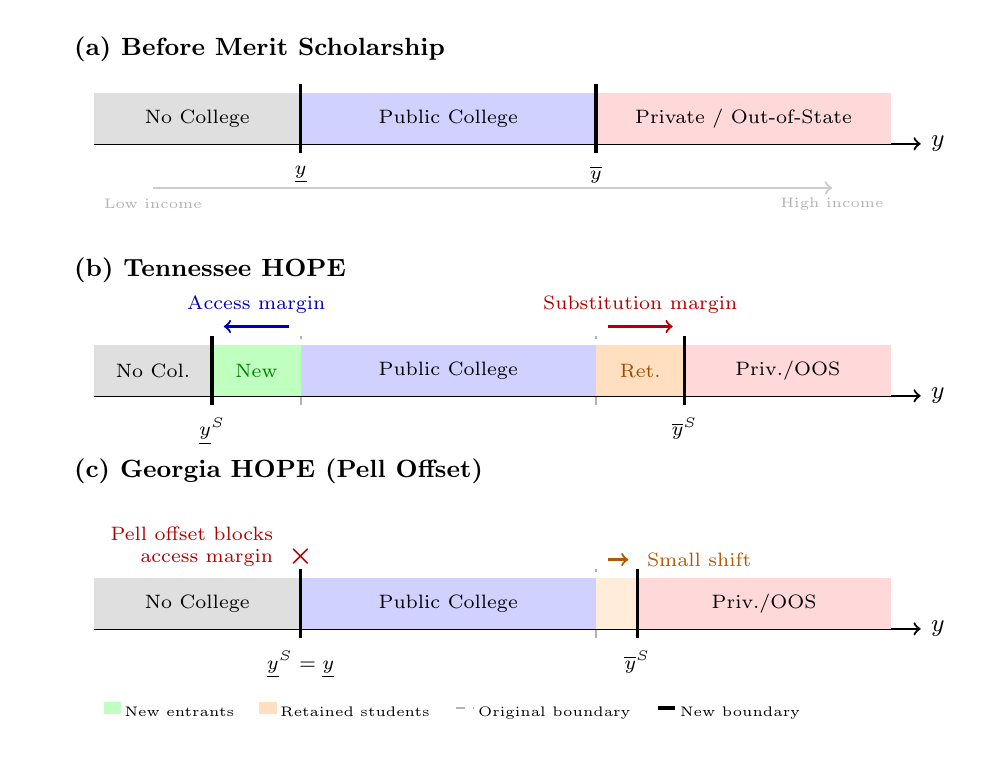
\begin{tikzpicture}[
  x=0.75cm, y=0.8cm,
  region/.style={minimum height=0.7cm, text=black, font=\scriptsize},
  boundary/.style={thick, dashed, gray!60},
  newboundary/.style={very thick, black},
  panellabel/.style={font=\small\bfseries, anchor=west},
  legendbox/.style={font=\tiny, anchor=west},
]

% ============================================================
% Panel A: Pre-Scholarship  (y = 12 to 14)
% ============================================================
\node[panellabel] at (-0.5, 13.0) {(a) Before Merit Scholarship};

% Income axis
\draw[thick, ->] (0, 11.5) -- (14, 11.5) node[right, font=\small] {$y$};

% Shaded regions
\fill[gray!25] (0, 11.5) rectangle (3.5, 12.3);
\fill[blue!18] (3.5, 11.5) rectangle (8.5, 12.3);
\fill[red!15] (8.5, 11.5) rectangle (13.5, 12.3);

% Region labels
\node[region] at (1.75, 11.9) {No College};
\node[region] at (6, 11.9) {Public College};
\node[region] at (11, 11.9) {Private / Out-of-State};

% Boundaries
\draw[very thick] (3.5, 11.35) -- (3.5, 12.45);
\draw[very thick] (8.5, 11.35) -- (8.5, 12.45);
\node[font=\scriptsize, below] at (3.5, 11.3) {$\underline{y}$};
\node[font=\scriptsize, below] at (8.5, 11.3) {$\overline{y}$};

% Income gradient
\draw[gray!40, thick, ->] (1, 10.8) -- (12.5, 10.8);
\node[font=\tiny, gray!60] at (1, 10.55) {Low income};
\node[font=\tiny, gray!60] at (12.5, 10.55) {High income};

% ============================================================
% Panel B: Post-Scholarship (Tennessee)  (y = 6 to 9.5)
% ============================================================
\node[panellabel] at (-0.5, 9.5) {(b) Tennessee HOPE};

% Income axis
\draw[thick, ->] (0, 7.5) -- (14, 7.5) node[right, font=\small] {$y$};

% Original boundaries (dashed)
\draw[boundary] (3.5, 7.35) -- (3.5, 8.45);
\draw[boundary] (8.5, 7.35) -- (8.5, 8.45);

% Shaded regions
\fill[gray!25] (0, 7.5) rectangle (2, 8.3);
\fill[green!25] (2, 7.5) rectangle (3.5, 8.3);
\fill[blue!18] (3.5, 7.5) rectangle (8.5, 8.3);
\fill[orange!25] (8.5, 7.5) rectangle (10, 8.3);
\fill[red!15] (10, 7.5) rectangle (13.5, 8.3);

% Region labels
\node[region] at (1, 7.9) {No Col.};
\node[region, green!50!black] at (2.75, 7.9) {New};
\node[region] at (6, 7.9) {Public College};
\node[region, orange!60!black] at (9.25, 7.9) {Ret.};
\node[region] at (11.75, 7.9) {Priv./OOS};

% New boundaries
\draw[newboundary] (2, 7.35) -- (2, 8.45);
\draw[newboundary] (10, 7.35) -- (10, 8.45);
\node[font=\scriptsize, below] at (2, 7.3) {$\underline{y}^S$};
\node[font=\scriptsize, below] at (10, 7.3) {$\overline{y}^S$};

% Arrows showing shifts
\draw[thick, ->, blue!70!black] (3.3, 8.6) -- (2.2, 8.6);
\node[font=\scriptsize, blue!70!black, above] at (2.75, 8.65) {Access margin};

\draw[thick, ->, red!70!black] (8.7, 8.6) -- (9.8, 8.6);
\node[font=\scriptsize, red!70!black, above] at (9.25, 8.65) {Substitution margin};

% ============================================================
% Panel C: Georgia (Pell Offset)  (y = 1.5 to 5.5)
% ============================================================
\node[panellabel] at (-0.5, 6.3) {(c) Georgia HOPE (Pell Offset)};

% Income axis
\draw[thick, ->] (0, 3.8) -- (14, 3.8) node[right, font=\small] {$y$};

% Original boundary (dashed, upper only — lower doesn't move)
\draw[boundary] (8.5, 3.65) -- (8.5, 4.75);

% Shaded regions
\fill[gray!25] (0, 3.8) rectangle (3.5, 4.6);
\fill[blue!18] (3.5, 3.8) rectangle (8.5, 4.6);
\fill[orange!15] (8.5, 3.8) rectangle (9.2, 4.6);
\fill[red!15] (9.2, 3.8) rectangle (13.5, 4.6);

% Region labels
\node[region] at (1.75, 4.2) {No College};
\node[region] at (6, 4.2) {Public College};
\node[region] at (11.35, 4.2) {Priv./OOS};

% Boundaries
\draw[newboundary] (3.5, 3.65) -- (3.5, 4.75);
\draw[newboundary] (9.2, 3.65) -- (9.2, 4.75);
\node[font=\scriptsize, below] at (3.5, 3.6) {$\underline{y}^S = \underline{y}$};
\node[font=\scriptsize, below] at (9.2, 3.6) {$\overline{y}^S$};

% Blocked access — red X and annotation to the LEFT, not above
\node[font=\normalsize, red!70!black] at (3.5, 4.95) {$\boldsymbol{\times}$};
\node[font=\scriptsize, red!70!black, anchor=east, text width=3cm, align=right] at (3.2, 5.1)
  {Pell offset blocks\\access margin};

% Small substitution arrow and annotation to the RIGHT
\draw[thick, ->, orange!70!black] (8.7, 4.9) -- (9.05, 4.9);
\node[font=\scriptsize, orange!70!black, anchor=west] at (9.2, 4.9) {Small shift};

% ============================================================
% Legend
% ============================================================
\node[legendbox] at (0, 2.5) {%
  \tikz[baseline=-0.5ex]{\fill[green!25] (0,0) rectangle (0.3,0.18);}\,New entrants \quad
  \tikz[baseline=-0.5ex]{\fill[orange!25] (0,0) rectangle (0.3,0.18);}\,Retained students \quad
  \tikz[baseline=-0.5ex]{\draw[thick, dashed, gray!60] (0,0.09) -- (0.3,0.09);}\,Original boundary \quad
  \tikz[baseline=-0.5ex]{\draw[very thick, black] (0,0.09) -- (0.3,0.09);}\,New boundary
};

\end{tikzpicture}

\caption{Three-Destination Sorting: How Merit Scholarships Reshape
  Institutional Composition}
\label{fig:sorting_model}

\vspace{1mm}
\begin{minipage}{0.92\textwidth}
  \footnotesize
  \textit{Notes:} Panel~(a) shows pre-scholarship sorting by family
  income $y$. Panel~(b) shows Tennessee HOPE: the scholarship reduces
  the effective price of public college, shifting the lower boundary
  left (access margin: low-income students enter) and the upper boundary
  right (substitution margin: high-income students retained in public
  rather than exiting to private). The public sector expands in both
  directions, producing progressive sorting. Panel~(c) shows Georgia
  HOPE: the Pell offset eliminates the effective subsidy for
  bottom-quintile families, so the lower boundary does not shift
  ($\times$). Only the upper boundary moves modestly, producing
  regressive sorting.
\end{minipage}
\end{figure}


\subsection{Testable Predictions}

The model generates seven predictions:

\begin{description}
\item[P1: Bottom-quintile share rises at public colleges.] The
  scholarship reduces the effective price of public college. Because
  $S / y_i$ is largest for low-income families, the marginal entrants
  drawn from below $\underline{y}$ are disproportionately low-income.
  We test P1 in Section~\ref{sec:results_main}.

\item[P2: Monotonic quintile gradient.] The price reduction $S / y_i$
  is monotonically decreasing in income. Q1 families experience the
  largest proportional price reduction; Q5 the smallest. The
  composition shift should be monotonically graded across quintiles.
  We test P2 in Section~\ref{sec:results_quintile}.

\item[P3: Composition change reflects sorting, not enrollment
  expansion.] Total enrollment at public colleges is unchanged if
  capacity constraints bind; the share shifts are driven by changes in
  who enrolls, not in how many enroll.
  We test P3 in Section~\ref{sec:results_mechanisms}.

\item[P4: No mirror image at private colleges.] If displaced
  top-quintile students exit to out-of-state options rather than
  shifting to private colleges, private institutions should show no
  significant composition change.
  We test P4 in Section~\ref{sec:results_mechanisms}.

\item[P5: Heterogeneous channels by tier.] At two-year colleges, where
  the no-college margin is active, the scholarship expands access
  (pulls in new students from below $\underline{y}$). At four-year
  universities, where the public/private margin is active, the
  scholarship induces sorting---a form of the ability stratification
  documented by \textcite{cornwell2006sorting}.
  We test P5 in Section~\ref{sec:results_mechanisms}.

\item[P6: Spatial heterogeneity.] Institutions located near state
  borders, where out-of-state alternatives are accessible, should show
  larger composition shifts because the outside option is more salient
  and the three-destination mechanism is most active.
  We test P6 in Section~\ref{sec:spatial}.

\item[P7: Cross-state variation.] Programs with no Pell offset and
  large public-private subsidy differentials produce progressive
  sorting. Programs with Pell offsets or comparable private awards
  produce regressive sorting or no composition change. The direction
  depends on whether the access margin operates for low-income
  students and whether $(S - s)$ is large enough to induce sector
  switching.
  We test P7 in Section~\ref{sec:discussion}.
\end{description}

\subsection{Reconciling with Dynarski (2000)}

\textcite{dynarski2000hope} finds that Georgia's HOPE Scholarship
widened the attendance gap between higher- and lower-income students.
Our framework shows that this aggregate finding is consistent with a
progressive composition shift at public institutions. Because
eligibility is correlated with income, merit aid increases the
\emph{total} number of higher-income students attending college more
than the total number of lower-income students. But the
\emph{destination} of these additional higher-income students matters.
If they enroll at private or out-of-state institutions---or if they
would have attended college anyway---the composition of public colleges
can still shift downward.

The reconciliation rests on distinguishing between two quantities: the
aggregate attendance gap (which can widen) and the institutional
composition of the public sector (which can simultaneously become more
progressive). Both are consistent with three-destination sorting.

This distinction is specific to the multi-sector setting. In a
two-sector model---attend college or not---the aggregate attendance
effect fully determines composition: if merit aid increases enrollment
disproportionately among higher-income students, those students
necessarily appear at colleges, and composition becomes more affluent.
With three or more destinations, the link breaks. Higher-income students
may attend college at higher rates but sort into private or out-of-state
institutions, leaving the public sector's composition to be determined
by the sorting behavior of remaining students. Individual enrollment
responses are therefore insufficient to predict institutional
composition; the full destination distribution is required. Our model
captures this by allowing sorting across all three margins
simultaneously.

\subsection{Georgia as a Regressive Prediction}
\label{sec:theory_georgia}

Georgia's HOPE included a Pell offset: scholarship dollars were reduced
dollar-for-dollar by Pell Grant receipts (Figure~\ref{fig:sorting_model}, Panel~C). Because Pell Grants target Q1
families, the effective scholarship for the poorest students was
\begin{equation}
  S_{\text{eff}}^{Q1} = \max(S - \text{Pell},\; 0) \approx 0.
\end{equation}
The model predicts no composition shift for Q1 (the price reduction is
zero), while Q3--Q5 families receive the full $S$. The predicted effect
is regressive: public colleges gain middle- and upper-income students
without gaining low-income students. \textcite{dynarski2000hope}
documents the consequence: Black students, who were disproportionately
Pell-eligible, showed no attendance gain, while white students gained
12.3 percentage points.

Georgia's HOPE also provided comparable awards to private colleges,
muting the public-private subsidy differential.
\textcite{cornwell2006enrollment} confirm the pattern: four-year private
enrollment in Georgia \emph{rose} by 13.2\% after HOPE, and two-thirds
of the four-year enrollment gain reflected reduced out-of-state
migration rather than new college-goers.

Tennessee's HOPE has no Pell offset, no income cap, and a large
public-private subsidy differential (full tuition at publics vs.\
\$3,000--\$4,000 at privates). Under these parameters, the model
predicts that the access margin and substitution margin both operate,
producing the progressive gradient we observe. The TN-GA contrast is
a pair of outcomes predicted by the same model under different
parameter values.


% ============================================================
%  SECTION 4: DATA
% ============================================================

\section{Data}
\label{sec:data}

\subsection{Chetty et al.\ (2020) Panel}

We use the college-level panel constructed by
\textcite{chetty2020mobility}, which links tax records and college
enrollment data to measure the parental income distribution of students
at each institution. The panel covers 2,202 colleges across 52 states
and territories for birth cohorts 1980--1991 (approximately
corresponding to college entry years 1998--2009). Students are assigned
to the institution attended at ages 19--22.

The primary analysis table (MRC Table~3) provides college-by-cohort
observations with measures of parental income rank and quintile shares.
We supplement this with institutional characteristics from MRC Table~10
(SAT scores, expenditures, enrollment, Barron's selectivity, HBCU and
flagship status, graduation rates). These characteristics capture the
dimensions of institutional quality that prior work has linked to
earnings premia \parencite{brewer1999elite, dale2002selective}.

\subsection{Sample Construction}

We define treated institutions as Tennessee public colleges. Tennessee
has 51 colleges in the data, of which 26 are public---19 two-year
institutions and 7 four-year institutions. Multi-campus systems appear
as distinct identifiers (56 per cohort), but we identify 26 unique
public colleges.

The control group comprises public colleges in states that did not adopt
broad-based merit scholarship programs during the analysis period. We
drop all 25 states classified as merit-program adopters by
\textcite{sjoquist2015state}. The remaining 26 control states contribute
6,289 college-cohort observations. Of the 312 possible Tennessee
public-college-by-cohort observations ($26 \times 12$), 291 are
non-missing on both primary outcomes.

We exclude 24 observations with missing state or institution type.

\subsection{Outcome Variables}

Our two primary outcomes are:

\begin{itemize}
\item \textbf{Bottom-quintile share} ($Q_1$): the fraction of students
  at college $c$ in cohort $t$ whose parents are in the bottom 20\% of
  the national income distribution. Baseline mean for Tennessee public
  colleges: 0.138.

\item \textbf{Mean parental income rank} ($\overline{r}$): the average
  percentile rank of parental household income for students at college
  $c$ in cohort $t$. Baseline mean for Tennessee publics: 0.540.
\end{itemize}

A clarification on the unit of observation: each outcome is measured at
the college-by-birth-cohort level, not for the entire enrolled student
body at a point in time. For example, $Q_1$ for the University of
Tennessee in cohort 1986 measures the fraction of all 1986-born students
who attended UT between ages 19 and 22 whose parents were in the bottom
quintile. The Fall 2006 student body at UT, by contrast, would include
birth cohorts 1984--1987 simultaneously---mixing untreated and treated
cohorts. The cohort-specific measure provides sharper identification
because it isolates students who faced HOPE-era incentives from those
who did not. By the end of the post-treatment window ($k = +5$, cohort
1991), nearly all cohorts enrolled at a given institution are treated, so
cohort-level and student-body-level effects converge.

For the quintile decomposition, we additionally use the share of
students from each income quintile ($Q_1$ through $Q_5$).

For the level decomposition that addresses ecological inference
concerns, we construct count outcomes by multiplying quintile shares by
cohort size. For example, Q1 count $= Q_1 \times N_{ct}$, where
$N_{ct}$ is total enrollment at college $c$ in cohort $t$.

\subsection{Summary Statistics}

Table~\ref{tab:summary_stats} reports summary statistics for the primary
outcomes and quintile shares, separately for Tennessee public colleges
and control-state public colleges. Tennessee publics have a somewhat
higher baseline share of bottom-quintile students (14.0\% vs.\ 13.6\%)
and lower mean parental income rank (0.524 vs.\ 0.541). The quintile
distribution at Tennessee publics is shifted leftward: Q1 and Q2 shares
are higher, Q5 share is lower. Table~\ref{tab:did_main} reports pre-
and post-treatment means. After HOPE implementation, bottom-quintile
share at Tennessee publics rises to 15.9\%, while the control group
increases modestly to 12.9\%. The raw difference-in-differences is 1.5
percentage points.

\begin{table}[H]
\centering
\begin{threeparttable}
\caption{Summary Statistics}
\label{tab:summary_stats}
\begin{tabular}{lcccc}
\toprule
 & \multicolumn{2}{c}{TN Public} & \multicolumn{2}{c}{Control Public} \\
\cmidrule(lr){2-3} \cmidrule(lr){4-5}
 & Mean & SD & Mean & SD \\
\midrule
\multicolumn{5}{l}{\textit{Primary Outcomes}} \\
\quad Bottom-quintile share ($Q_1$) & 0.140 & 0.046 & 0.136 & 0.083 \\
\quad Mean parental income rank & 0.524 & 0.067 & 0.541 & 0.103 \\
\addlinespace
\multicolumn{5}{l}{\textit{Quintile Shares}} \\
\quad Q1 (bottom) & 0.140 & & 0.136 & \\
\quad Q2 & 0.195 & & 0.182 & \\
\quad Q3 & 0.239 & & 0.227 & \\
\quad Q4 & 0.256 & & 0.252 & \\
\quad Q5 (top) & 0.170 & & 0.203 & \\
\addlinespace
Observations & \multicolumn{2}{c}{137} & \multicolumn{2}{c}{2,850} \\
Colleges & \multicolumn{2}{c}{26} & \multicolumn{2}{c}{$\sim$500} \\
\bottomrule
\end{tabular}
\begin{tablenotes}[flushleft]
\footnotesize
\item \textit{Notes:} Pre-treatment means (birth cohorts 1980--1985)
  for Tennessee public colleges (treated) and public colleges in 26
  non-merit-program states (control). Quintile shares refer to the
  fraction of students whose parents are in the indicated quintile of
  the national income distribution. Observations are at the
  college-by-cohort level. Data: \textcite{chetty2020mobility}.
\end{tablenotes}
\end{threeparttable}
\end{table}


% ============================================================
%  SECTION 5: EMPIRICAL STRATEGY
% ============================================================

\section{Empirical Strategy}
\label{sec:empirical_strategy}

\subsection{Primary Estimator: Callaway and Sant'Anna (2021)}

Our primary estimator is the group-time average treatment effect on the
treated (ATT) proposed by \textcite{callaway2021difference}. This
estimator avoids the negative weighting and heterogeneity bias that
can afflict two-way fixed effects specifications when treatment effects
vary over time \parencite{goodmanbacon2021difference,
sun2021estimating}.

In our setting, treatment timing is sharp: all Tennessee public colleges
are treated simultaneously at $t^* = 1986$ (the first birth cohort with
unambiguous HOPE exposure). The Callaway--Sant'Anna estimator computes
group-time ATTs by comparing the outcome evolution of the treated group
to a ``never-treated'' comparison group. We aggregate the group-time
ATTs into an overall ATT and dynamic event-study coefficients.

We report TWFE event-study estimates for comparability with the prior
difference-in-differences literature
\parencite{ashenfelter1985panel, card1994minimum}. The TWFE
specification is:

\begin{equation}
y_{ct} = \alpha_c + \lambda_t + \sum_{k=-5}^{5} \beta_k \cdot
\mathbf{1}[t - t^* = k] \cdot \text{Treated}_c + \varepsilon_{ct}
\label{eq:twfe}
\end{equation}

\noindent where $y_{ct}$ is the outcome for college $c$ in birth cohort
$t$, $\alpha_c$ are college fixed effects, $\lambda_t$ are cohort fixed
effects, $\text{Treated}_c$ indicates Tennessee public colleges, and
$k = -1$ is the omitted reference period.

\subsection{Identification}

Identification requires that Tennessee public colleges would have
followed parallel trends in socioeconomic composition to control
colleges absent the HOPE Scholarship. We assess this assumption in
three ways.

First, we inspect pre-treatment event-study coefficients. Under the
national control group, coefficients at $k = -5$ through $k = -3$ show
some divergence from zero for bottom-quintile share, raising concerns about
longer-horizon pre-trends. The $k = -5$ coefficient is driven by a
single cohort (1980 births) and its magnitude is sensitive to the
inclusion of this endpoint.

Second, we implement a bordering-state control group that restricts
comparisons to colleges in states adjacent to Tennessee. This
specification passes pre-trend tests: pre-treatment coefficients are
small, statistically insignificant, and show no systematic pattern.
The bordering-state specification is our preferred identification
strategy.

Third, we implement a conservative control group that drops states with
any policy changes in higher education funding during the analysis
window. Results are quantitatively similar to the baseline.

\subsection{Inference}

Standard errors are clustered at the state level, the level at which
treatment is assigned. With 27 clusters (26 control states plus
Tennessee), we are near the boundary where cluster-robust inference
becomes unreliable. In the Callaway--Sant'Anna framework, we use
the analytical standard errors provided by the \texttt{csdid} package,
which account for the two-step estimation.

For the bordering-state specification, which has only four state
clusters ($G_1 = 1$ treated), the wild cluster bootstrap is
uninformative \parencite{mackinnon2017wild}. We therefore supplement
analytical standard errors with a Fisher-style permutation test that
assigns placebo treatment to each state in turn and ranks Tennessee's
estimate against the resulting distribution. We report permutation
$p$-values in Section~\ref{sec:robustness_permutation}.

\subsection{Sensitivity Analysis}

We implement the honest confidence intervals of
\textcite{rambachan2023more}, which relax the parallel trends assumption
by allowing for bounded violations. We report results under two restrictions:

\begin{itemize}
\item \textbf{Relative magnitude} ($\Delta_\text{RM}$): post-treatment
  violations of parallel trends are bounded by a multiple $\bar{M}$ of
  the maximum pre-treatment violation. Results remain significant at
  $\bar{M} \leq 2$ for bottom-quintile share.

\item \textbf{Smoothness} ($\Delta_\text{SD}$): consecutive violations
  of parallel trends are bounded in their rate of change. Under this
  restriction, confidence intervals include zero at moderate bounds,
  indicating fragility. We interpret this as a limitation: if
  differential trends can accelerate smoothly, our estimates cannot be
  distinguished from pre-existing dynamics.
\end{itemize}

We discuss these results in detail in Section~\ref{sec:robustness} and
interpret the tension between $\Delta_\text{RM}$ and $\Delta_\text{SD}$
as informative about the nature of potential confounds.

\subsection{Synthetic Control}

As a complementary identification strategy, we implement the synthetic
control method \parencite{abadie2010synthetic}, which constructs a
data-driven counterfactual for Tennessee by selecting weighted
combinations of donor states that best match Tennessee's pre-treatment
composition trends. The donor pool consists of 22 non-merit states,
matching on pre-treatment bottom-quintile share levels (birth cohorts
1980--1984). This approach avoids imposing equal weights across all
control states and directly addresses concerns about the suitability of
any particular comparison group. We report the synthetic control trends
in Section~\ref{sec:results} and placebo-in-space inference in
Section~\ref{sec:robustness_synth}.


% ============================================================
%  SECTION 6: RESULTS
% ============================================================

\section{Results}
\label{sec:results}

\subsection{Main Effects}
\label{sec:results_main}

Figures~\ref{fig:synth_trends_par_q1}
and~\ref{fig:synth_trends_par_rank} provide visual evidence of the
compositional shift. The synthetic control, constructed from a weighted
combination of non-merit states
\parencite{abadie2010synthetic}, matches Tennessee almost exactly
through the pre-treatment period (1980--1984) for both outcomes. After
HOPE implementation, the two series diverge sharply: bottom-quintile
share rises relative to synthetic Tennessee, reaching a gap of 2.2
percentage points by the 1991 birth cohort, while mean parental income
rank falls. The pre-treatment fit is excellent for both outcomes, with
near-zero root mean squared prediction error.

\begin{figure}[t]
  \centering
  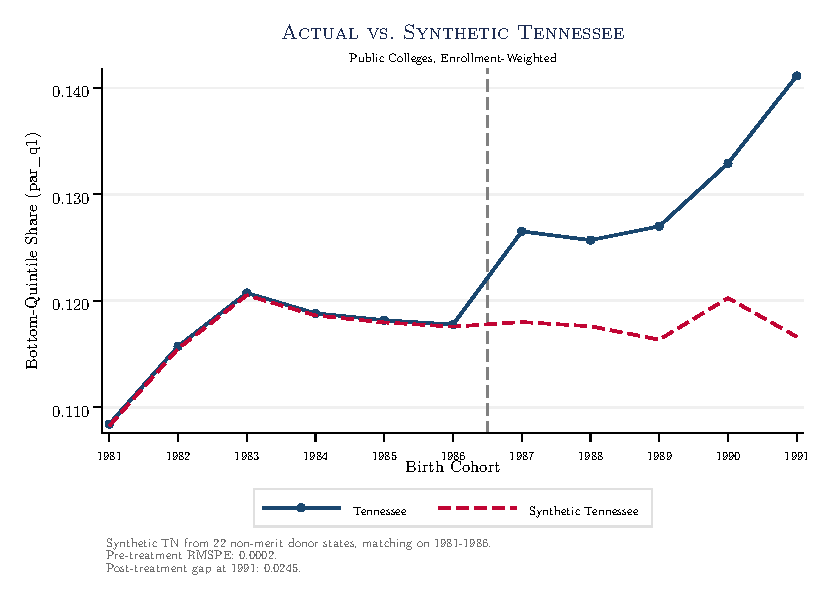
\includegraphics[width=0.85\textwidth]{fig_synth_trends_par_q1.pdf}
  \caption{Actual vs.\ Synthetic Tennessee: Bottom-Quintile Share at
    Public Colleges}
  \label{fig:synth_trends_par_q1}
  \vspace{1mm}
  \begin{minipage}{0.85\textwidth}
    \footnotesize
    \textit{Notes:} Synthetic Tennessee is constructed from a weighted
    combination of 22 non-merit states using the method of
    \textcite{abadie2010synthetic}, matching on pre-treatment
    bottom-quintile share (1980--1984). The vertical dashed line
    indicates the first HOPE-eligible birth cohort. The two series track
    closely in the pre-treatment period, then diverge after HOPE
    implementation. Data: \textcite{chetty2020mobility}.
  \end{minipage}
\end{figure}

\begin{figure}[t]
  \centering
  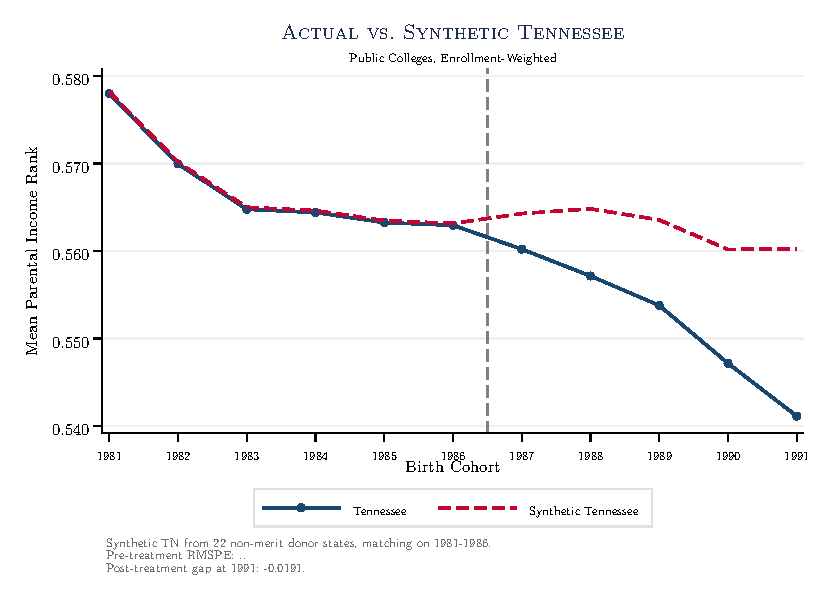
\includegraphics[width=0.85\textwidth]{fig_synth_trends_par_rank.pdf}
  \caption{Actual vs.\ Synthetic Tennessee: Mean Parental Income Rank at
    Public Colleges}
  \label{fig:synth_trends_par_rank}
  \vspace{1mm}
  \begin{minipage}{0.85\textwidth}
    \footnotesize
    \textit{Notes:} Synthetic Tennessee constructed as in
    Figure~\ref{fig:synth_trends_par_q1}, matching on pre-treatment
    mean parental income rank (1980--1984). Tennessee's actual parental
    income rank diverges downward after HOPE implementation, consistent
    with the progressive compositional shift documented in the
    bottom-quintile share results. Data: \textcite{chetty2020mobility}.
  \end{minipage}
\end{figure}

Table~\ref{tab:cs_main} reports the Callaway--Sant'Anna aggregate ATT
estimates. Following HOPE implementation, the share of bottom-quintile
students at Tennessee public colleges increased by 1.27 percentage points (SE =
0.0026, $p < 0.001$) and decreased mean parental income rank by 1.33
percentage points (SE = 0.0020, $p < 0.001$). Both effects are precisely estimated
and economically meaningful: the bottom-quintile share increase
represents a 9.2\% gain relative to the pre-treatment mean of 13.8\%.
In levels, the effect corresponds to approximately 11.2 additional
bottom-quintile students per cohort at each Tennessee public college and
34.4 fewer top-quintile students per cohort
(Section~\ref{sec:results_mechanisms}). Across 26 treated public
colleges, this implies roughly 290 additional low-income students and
890 fewer high-income students per birth cohort gaining access to or
exiting the public system. The effect grows with exposure horizon:
by $k = +5$ (the 1991 birth cohort), the treatment effect reaches
$+3.1$ percentage points, a 22\% gain over baseline. This growing path
reflects intensifying program impact on successive cohorts rather than
mechanical accumulation, since each cohort's composition is measured
independently (Section~\ref{sec:data}).

For comparison, the static TWFE estimator yields slightly larger point
estimates---1.54 pp for bottom-quintile share and $-1.85$ pp for
mean parental income rank (Table~\ref{tab:twfe_did})---consistent with the
known upward bias of TWFE in the presence of dynamic treatment effects.
The qualitative conclusions are identical across estimators.

These share changes reflect real compositional sorting rather than an
enrollment artifact. We confirm in Section~\ref{sec:results_mechanisms}
that the number of bottom-quintile students per cohort increases by 11.2
($p = 0.014$), the number of top-quintile students per cohort decreases
by 34.4 ($p < 0.001$), and total enrollment is unchanged ($-2.1$,
$p = 0.93$). The public sector absorbs more lower-income students while
losing upper-income students, with the total headcount held constant.

\subsection{Event Study Dynamics}
\label{sec:results_dynamics}

Figure~\ref{fig:four_estimators} presents the event-study estimates
across four heterogeneity-robust estimators
(Section~\ref{sec:robustness_estimators}). Focusing on the
Callaway--Sant'Anna path, for bottom-quintile share the
treatment effect is near zero at $k = 0$ and grows monotonically to
approximately 2.5 percentage points by $k = 5$. For parental income rank,
the trajectory is symmetric: a gradual decline reaching $-2.6$ points
by $k = 5$.

The growing post-treatment path is consistent with an intensifying
compositional shift across successive cohorts. Because each birth
cohort's composition is measured independently in the
\textcite{chetty2020mobility} data, the increasing treatment effect
reflects deeper program impact on later cohorts---through rising
take-up, greater awareness, and institutional adaptation---rather than
mechanical accumulation of treated students in a fixed enrollment stock.

Pre-treatment coefficients under the bordering-state control group are
centered around zero with no systematic trend
(Figure~\ref{fig:four_estimators}). Under the national control group,
pre-treatment coefficients at $k = -5$ and $k = -4$ show some
divergence, as discussed in Section~\ref{sec:empirical_strategy}.

\subsection{Quintile Decomposition}
\label{sec:results_quintile}

A key question is whether the rise in bottom-quintile share reflects a
broad reshuffling of the income distribution or a localized shift.
Table~\ref{tab:quintile_decomp} decomposes the composition effect
across all five income quintiles using the TWFE static specification.

The results reveal a strikingly monotonic gradient:

\begin{center}
\begin{tabular}{lccl}
\toprule
Quintile & Coefficient & SE & \\
\midrule
Q1 (bottom) & $+0.0154$ & $(0.0030)$ & $^{***}$ \\
Q2 & $+0.0114$ & $(0.0025)$ & $^{***}$ \\
Q3 & $+0.0047$ & $(0.0018)$ & $^{*}$ \\
Q4 & $-0.0136$ & $(0.0021)$ & $^{***}$ \\
Q5 (top) & $-0.0179$ & $(0.0025)$ & $^{***}$ \\
\bottomrule
\end{tabular}
\end{center}

Every quintile's coefficient has the predicted sign, and the gradient
is monotonically ordered: $|\hat\beta_1| > |\hat\beta_2| >
|\hat\beta_3|$ and $|\hat\beta_5| > |\hat\beta_4|$. The bottom three
quintiles gain share at public colleges; the top two lose share.
Statistical significance is strongest at the tails (Q1 and Q5) and
weakest in the middle (Q2 and Q3). This pattern is expected for two
reasons. First, the theoretical mechanism generates the largest effects
at the extremes: the proportional price reduction $S/y_i$ is largest
for the lowest-income families and the substitution incentive is
strongest for the highest-income families, while middle-quintile
families experience smaller behavioral responses in both directions.
Second, the tails of the income distribution exhibit greater
cross-college variance---bottom- and top-quintile shares vary more
across institutions than middle-quintile shares, which cluster near
0.20---giving the estimator more identifying variation. The combination
of larger true effects and greater statistical power at the extremes
means that Q1 and Q5 are precisely estimated, Q4 is significant, and
Q2--Q3 are directionally consistent but noisier.\footnote{Under the
Callaway--Sant'Anna estimator, Q2 is significant ($p < 0.001$) but Q3
is not ($p = 0.38$). Under TWFE, all five are significant. Under the
bordering-state specification with three estimators
(Figure~\ref{fig:quintile_event_studies}, Appendix), Q1 and Q5 are
significant across all estimators, Q4 is significant under TWFE and
Sun--Abraham, and Q2--Q3 are directionally consistent. The monotonic
ordering of point estimates is preserved across all specifications.}

\begin{figure}[t]
  \centering
  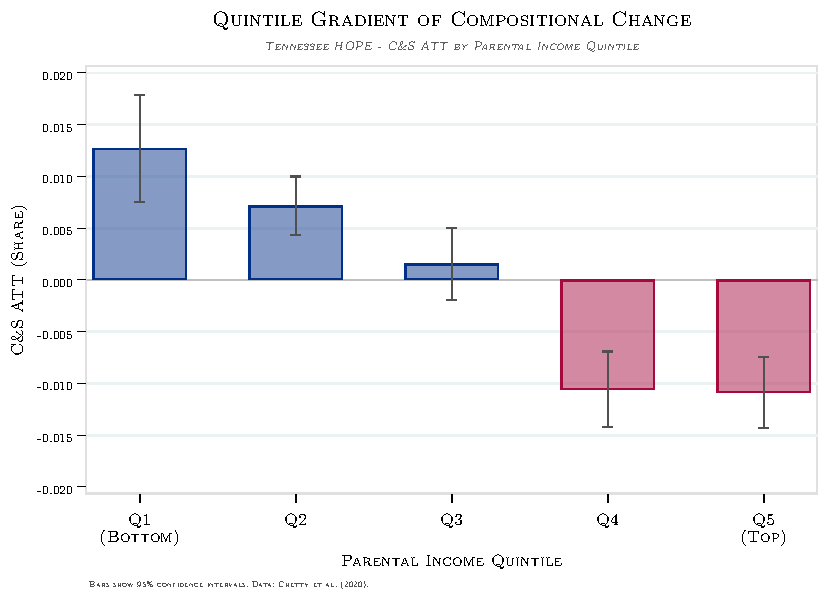
\includegraphics[width=0.75\textwidth]{fig_tn_quintile_gradient.pdf}
  \caption{Quintile Gradient of Compositional Change Following
    Tennessee HOPE}
  \label{fig:quintile_gradient}
  \vspace{1mm}
  \begin{minipage}{0.75\textwidth}
    \footnotesize
    \textit{Notes:} \textcite{callaway2021difference} ATT estimates for
    each parental income quintile share. The effect is monotonically
    ordered: bottom-quintile students gain the most representation and
    top-quintile students lose the most. Significance is strongest at the
    tails (Q1, Q5) where both the theoretical effect and cross-college
    variance are largest. Bars denote 95\% confidence intervals.
    Data: \textcite{chetty2020mobility}.
  \end{minipage}
\end{figure}

Figure~\ref{fig:quintile_gradient} displays the quintile gradient
graphically. The coefficients descend smoothly from Q1 ($+1.3$ pp)
through Q3 ($+0.2$ pp) to Q5 ($-1.1$ pp). The quintile-specific
event studies (Figure~\ref{fig:quintile_event_studies}, Appendix)
confirm that all five quintiles exhibit gradual divergence after
treatment onset, with three estimators agreeing on the direction and
dynamics at each quintile.

The quintile shares sum to one by construction. The finding that Q1
gains the most share and Q5 loses the most share implies that the
composition shift is driven by reallocation between the extremes of
the income distribution rather than by changes near the median. The
monotonic gradient also serves as a discriminating test of the HOPE
channel: a generic Tennessee-specific shock---whether driven by state
fiscal conditions, demographic trends, or concurrent reforms---would be
unlikely to produce five coefficients that are perfectly ordered in
magnitude. This specific pattern is a unique prediction of the
price-reduction mechanism in the three-destination model, where the
proportional cost reduction $S/y_i$ is monotonically decreasing in
income.

\subsection{Mechanism Evidence}
\label{sec:results_mechanisms}

\subsubsection{Level Decomposition: Shares vs.\ Counts}

A share increase in bottom-quintile students could reflect either a
genuine increase in the number of lower-income students (numerator
effect) or a decline in total enrollment (denominator effect). We
address this ecological inference concern by estimating effects on
count outcomes: Q1 count (number of bottom-quintile students per
cohort), Q5 count, and total enrollment.\footnote{Count outcomes are
constructed as quintile share $\times$ cohort enrollment. Because
enrollment varies substantially across colleges (coefficient of
variation $\approx 1.0$), count-based estimates are considerably
noisier than share-based estimates. The critical test is whether
\emph{total} enrollment changes, which is well-powered because it does
not inherit share-level noise. The directional signs of Q1 and Q5 counts
provide supporting evidence but should be interpreted with appropriate
caution given the wider confidence intervals.}

The critical finding is that total enrollment at Tennessee public
colleges is essentially unchanged after HOPE ($-2.1$ students per
cohort, $p = 0.93$). This rules out the denominator-artifact
explanation: the share changes cannot be driven by enrollment
contraction. The directional evidence is consistent with real
compositional sorting: Q1 count increases by 11.2 per cohort ($p =
0.014$) and Q5 count decreases by 34.4 per cohort ($p < 0.001$),
indicating that more bottom-quintile students enter the public sector
while more top-quintile students exit, with the total headcount held
constant (Table~\ref{tab:level_decomp}).

\subsubsection{Tier Heterogeneity}

Table~\ref{tab:tier_het} reports separate estimates for two-year and
four-year institutions.

At two-year colleges, the bottom-quintile share increases by 1.81
percentage points (SE = 0.0034, $p < 0.001$) and mean parental income
rank falls by 1.73 percentage points. These institutions show a loss of 22.9 Q5
students per cohort ($p = 0.001$) but no significant change in total
enrollment. The evidence is consistent with \emph{displacement}: lower-income
students replace higher-income students at community colleges, with the
overall seat count unchanged.

At four-year colleges, the bottom-quintile share increases by a smaller
0.70 percentage points (SE = 0.0024, $p = 0.008$), but total enrollment
increases by 138.5 students per cohort ($p < 0.001$). Four-year
institutions gain 19.6 Q1 students and lose 39.2 Q5 students. The evidence is consistent with \emph{expansion}: these institutions
grow their enrollment while simultaneously experiencing downward
compositional sorting.

The two tiers thus exhibit different adjustment channels, consistent
with Prediction P5. Community colleges adjust on the intensive margin
(who fills existing seats), while four-year institutions adjust on
the extensive margin (adding seats while changing composition).

\subsubsection{Tennessee Privates: No Spillover}

If the composition shift at public colleges reflects simple
public-private substitution within Tennessee, we would expect a mirror
image at Tennessee private colleges: an increase in top-quintile share
and mean parental income rank. We test this directly.

Table~\ref{tab:spillover} reports Callaway--Sant'Anna ATTs comparing
Tennessee private colleges to private colleges in control states. The
effect on bottom-quintile share is 0.11 percentage points (SE = 0.0011,
$p = 0.30$)---small, positive, and statistically insignificant. The
effect on mean parental income rank is $-0.46$ percentage points (SE = 0.0018, $p =
0.016$), marginally significant but in the same direction as the
public-sector effect rather than the opposite direction.

Tennessee private colleges do not absorb the top-quintile students who
leave the public sector. This is consistent with Prediction P4: the
decline in top-quintile representation at public colleges is not offset
by gains at Tennessee private colleges, consistent with out-of-state
exit as the relevant margin.
Figure~\ref{fig:pub_vs_priv} displays the contrast visually:
the public-sector event study shows a clear progressive shift while
the private-sector event study is flat, confirming that the
compositional change is specific to the public sector.
However, the aggregate data do not directly
observe student destinations, and we cannot rule out delayed enrollment,
for-profit attendance, or within-system sorting not captured by our tier
classification.

\begin{figure}[H]
  \centering
  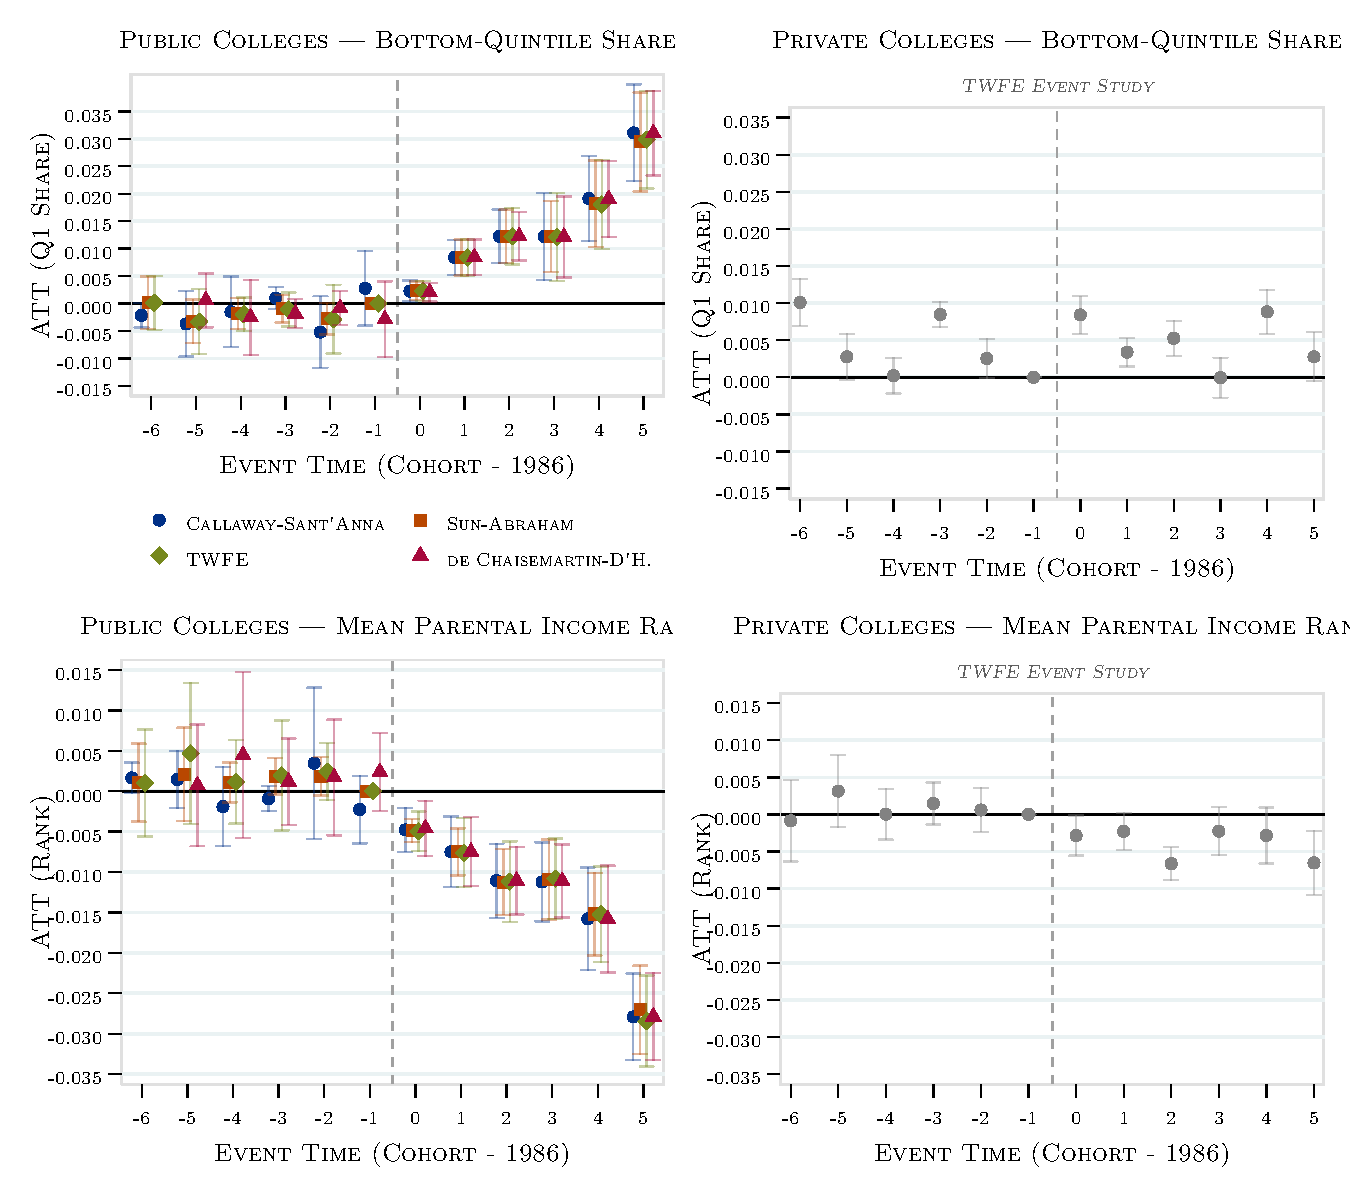
\includegraphics[width=\textwidth]{fig_public_vs_private_2x2_combined.pdf}
  \caption{Public vs.\ Private Colleges: Event Studies for Both Outcomes}
  \label{fig:pub_vs_priv}
  \vspace{1mm}
  \begin{minipage}{\textwidth}
    \footnotesize
    \textit{Notes:} Left column: four heterogeneity-robust estimators
    for Tennessee public colleges vs.\ public colleges in 26 non-merit
    states. Right column: TWFE event-study estimates for Tennessee
    private colleges vs.\ private colleges in control states. Top row:
    bottom-quintile share. Bottom row: mean parental income rank.
    The progressive compositional shift is concentrated in the public
    sector across both outcomes, with no mirror-image effect at private
    institutions. Vertical bars denote 95\% confidence intervals.
    Data: \textcite{chetty2020mobility}.
  \end{minipage}
\end{figure}

\subsubsection{Where Did Top-Quintile Students Go?}

The tier heterogeneity results (Table~\ref{tab:tier_het}) shed light on
the Q5 exit pattern. Two-year colleges lost 22.9 Q5 students per cohort
($p = 0.001$) with no significant enrollment change, while four-year
colleges lost 39.2 Q5 students ($p = 0.034$) alongside enrollment
\emph{growth} of 138.5 students ($p < 0.001$). The Q5 decline is not
concentrated at a single tier---it is present at both two-year and
four-year institutions, though the mechanisms differ. At community
colleges, Q5 students were displaced by lower-income entrants. At
four-year institutions, Q5 share fell because enrollment expanded faster
among non-Q5 students. In neither case do the displaced Q5 students appear at Tennessee private
colleges, reinforcing the interpretation that the relevant exit margin
is outside Tennessee's private sector.


\subsubsection{Within-Tennessee Public vs.\ Private Comparison}

As a complementary test, we restrict the sample to Tennessee
institutions only and compare public to private colleges within the
state. This eliminates any concerns about cross-state confounds.

The within-Tennessee DiD estimate for bottom-quintile share is 1.42
percentage points (SE = 0.0037, $p < 0.001$) and for mean parental income rank
is $-2.14$ percentage points (SE = 0.0032, $p < 0.001$). These estimates are
slightly larger than the cross-state estimates, consistent with
Tennessee private colleges serving as a clean within-state control.
The sample is small ($N = 571$), but the effects are precisely estimated
and confirm that the composition shift is specific to the public sector.

\subsection{Spatial Heterogeneity}
\label{sec:spatial}

The three-destination model predicts that the composition shift varies
with institutional geography (P6). Colleges closer to state borders
face stronger outside-option competition---the kind of cross-market
pressure emphasized by \textcite{hoxby2000peer}---which should amplify
the sorting mechanism. We test this prediction by estimating heterogeneous
effects along two spatial dimensions: border proximity and region.

\textbf{Border vs.\ interior.} Institutions in Tennessee counties that
border another state show a 38\% larger progressive shift than interior
institutions: the bottom-quintile share ATT is $+1.89$ pp (SE $=
0.003$, $p < 0.001$) at border colleges versus $+1.37$ pp (SE $=
0.003$, $p < 0.001$) at interior colleges. The monotonic quintile
gradient holds in both subsamples, but the gradient is steeper at
border colleges. This is consistent with P6: where students have
accessible out-of-state alternatives, HOPE's price reduction has a
larger behavioral effect on the margin between public enrollment and
exit.

\textbf{Regional variation.} The effect varies strikingly across
Tennessee's three Grand Divisions (Table~\ref{tab:spatial}). West
Tennessee shows the largest shift ($+3.13$ pp, $p < 0.001$), roughly
triple the magnitude in East Tennessee ($+1.13$ pp, $p < 0.001$) and
Middle Tennessee ($+1.03$ pp, $p = 0.002$). The monotonic quintile
gradient holds in all three regions. The concentration in West
Tennessee---where the Memphis metropolitan area's proximity to
Mississippi and Arkansas creates strong cross-border competition, and a
high density of community colleges favors both access expansion and
competitive retention---is consistent with the model's spatial
predictions.\footnote{West Tennessee contains only 6 of the 26 public
colleges. The large point estimate should be interpreted with this
small-sample caveat in mind.}

Figure~\ref{fig:spatial_map} displays the geographic distribution of
the effect. Each of Tennessee's 26 public colleges is marked at its
county location, with the county fill reflecting the regional ATT
magnitude. The concentration of the effect in West Tennessee---and
particularly in border counties adjacent to Mississippi and
Arkansas---is visually striking.

\begin{figure}[H]
  \centering
  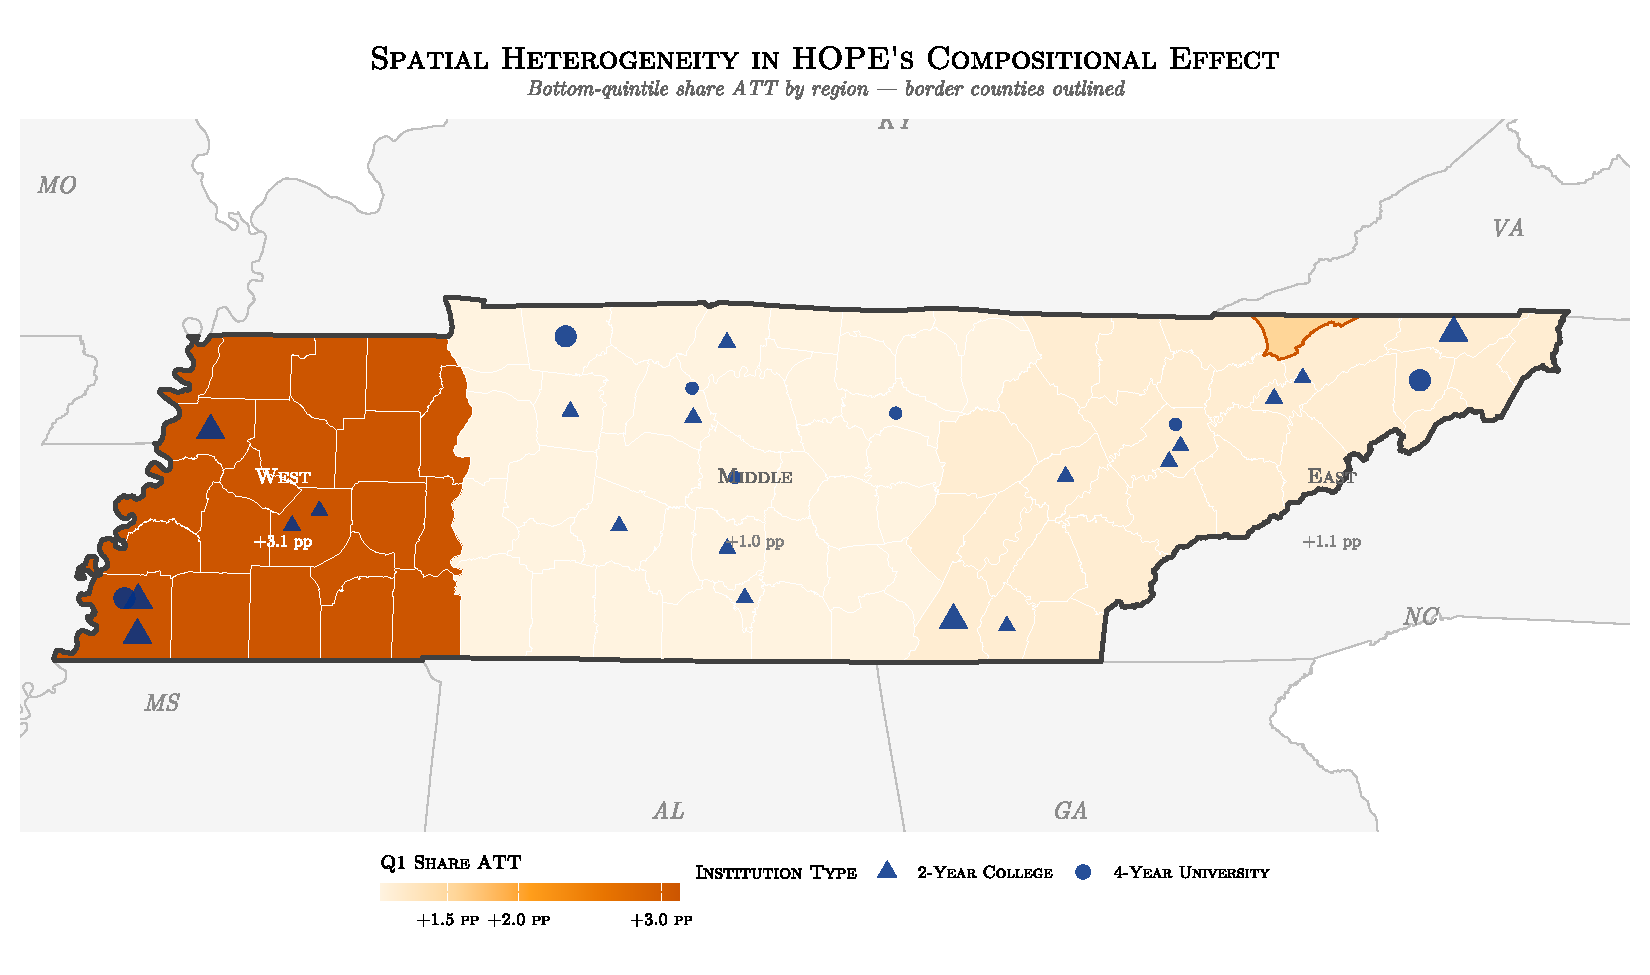
\includegraphics[width=\textwidth]{fig_spatial_heterogeneity.pdf}
  \caption{Geographic Distribution of HOPE's Compositional Effect}
  \label{fig:spatial_map}
  \vspace{1mm}
  \begin{minipage}{\textwidth}
    \footnotesize
    \textit{Notes:} County fill reflects the regional bottom-quintile
    share ATT (West: $+3.1$ pp, East: $+1.1$ pp, Middle: $+1.0$ pp),
    with border counties receiving a 38\% boost per the border vs.\
    interior heterogeneity estimate. Navy markers indicate public
    college locations: circles = four-year universities, triangles =
    two-year colleges. Border counties are outlined. Neighboring states
    labeled to illustrate out-of-state exit destinations.
    Data: \textcite{chetty2020mobility}.
  \end{minipage}
\end{figure}

\begin{table}[t]
\centering
\begin{threeparttable}
\caption{Spatial Heterogeneity in HOPE's Compositional Effect}
\label{tab:spatial}
\begin{tabular}{lccc}
\toprule
 & Q1 Share ATT & SE & Colleges \\
\midrule
\textit{By Border Status} & & & \\
\quad Border counties & $0.0189^{***}$ & $(0.003)$ & 8 \\
\quad Interior counties & $0.0137^{***}$ & $(0.003)$ & 18 \\
\midrule
\textit{By Region} & & & \\
\quad East Tennessee & $0.0113^{***}$ & $(0.003)$ & 9 \\
\quad Middle Tennessee & $0.0103^{**}$ & $(0.003)$ & 11 \\
\quad West Tennessee & $0.0313^{***}$ & $(0.003)$ & 6 \\
\bottomrule
\end{tabular}
\begin{tablenotes}[flushleft]
\footnotesize
\item \textit{Notes:} TWFE static difference-in-differences estimates.
  College and cohort fixed effects included. Standard errors clustered
  at the state level in parentheses. Border counties share a boundary
  with another state. Regional definitions follow Tennessee's Grand
  Divisions. $^{***}p<0.01$, $^{**}p<0.05$, $^{*}p<0.10$.
  Data: \textcite{chetty2020mobility}.
\end{tablenotes}
\end{threeparttable}
\end{table}

\subsection{Summary of Theoretical Predictions}

Table~\ref{tab:predictions} maps each prediction from the
three-destination model to its empirical test and result.

\begin{table}[H]
\centering
\begin{threeparttable}
\caption{Model Predictions and Empirical Tests}
\label{tab:predictions}
\begin{tabular}{llll}
\toprule
Prediction & Test & Section & Result \\
\midrule
P1: Q1 share rises & C\&S ATT & \ref{sec:results_main} & $+1.27$ pp ($p < 0.001$) \\
P2: Monotonic gradient & Quintile decomp. & \ref{sec:results_quintile} & 5/5 ordered \\
P3: Sorting, not expansion & Level decomp. & \ref{sec:results_mechanisms} & Total $\Delta = -2.1$ ($p = 0.93$) \\
P4: No mirror at privates & Spillover test & \ref{sec:results_mechanisms} & Null ($p = 0.30$) \\
P5: Tier heterogeneity & 2-yr vs.\ 4-yr & \ref{sec:results_mechanisms} & Different channels \\
P6: Spatial gradient & Border vs.\ interior & \ref{sec:spatial} & Border 38\% larger \\
P7: Cross-state variation & TN, GA, WV & \ref{sec:discussion} & Design predicts direction \\
\bottomrule
\end{tabular}
\begin{tablenotes}[flushleft]
\footnotesize
\item \textit{Notes:} Predictions are derived in Section~\ref{sec:theory}.
  All Tennessee results use the preferred treatment timing ($t^* = 1986$).
  P7 is evaluated in the Discussion using cross-state evidence.
\end{tablenotes}
\end{threeparttable}
\end{table}


% ============================================================
%  SECTION 7: ROBUSTNESS
% ============================================================

\section{Robustness}
\label{sec:robustness}

\subsection{Alternative Estimators}
\label{sec:robustness_estimators}

We compare four heterogeneity-robust difference-in-differences
estimators: Callaway--Sant'Anna
\parencite{callaway2021difference}, \textcite{sun2021estimating},
TWFE (Equation~\ref{eq:twfe}), and
\textcite{dechaisemartin2020two}. Each estimator addresses the
heterogeneous treatment effects problem through a different approach:
Callaway--Sant'Anna computes group-time ATTs relative to never-treated
units; Sun--Abraham uses interaction-weighted estimation;
de~Chaisemartin--D'Haultfoeuille applies a first-difference
estimator. TWFE is included for comparability with the prior literature
despite its known sensitivity to treatment effect heterogeneity
\parencite{goodmanbacon2021difference}.

Figure~\ref{fig:four_estimators} overlays all four estimators' dynamic
paths for both outcomes. TWFE and Sun--Abraham coefficients are
plotted relative to the omitted period ($k = -1$). Callaway--Sant'Anna
and de~Chaisemartin--D'Haultfoeuille estimates are group-time ATTs
relative to the never-treated comparison group, which do not require
a reference period. The four estimators agree on sign, magnitude, and
dynamics. Pre-treatment coefficients are statistically indistinguishable
from zero under all four estimators. Post-treatment coefficients
diverge monotonically and are statistically significant at every event
time from $k = 0$ onward.

\begin{figure}[H]
  \centering
  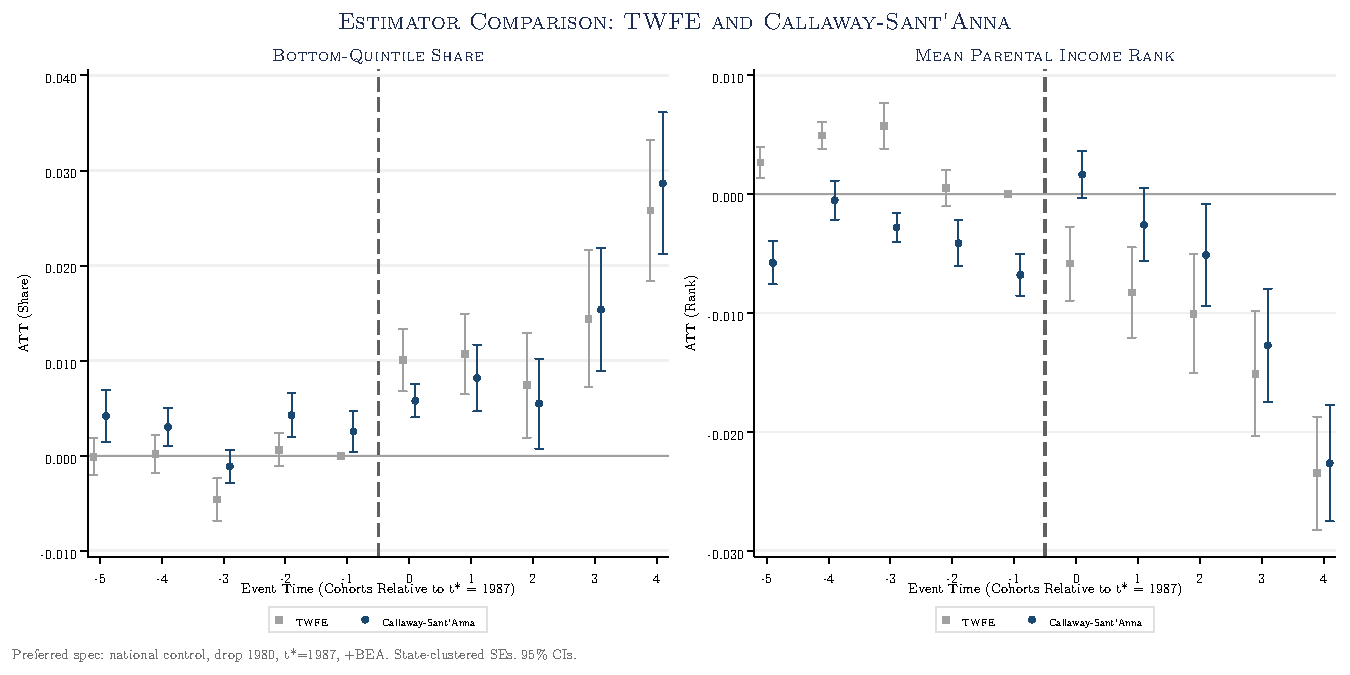
\includegraphics[width=\textwidth]{fig_four_estimators_combined.pdf}
  \caption{Robustness Across Four Heterogeneity-Corrected DiD Estimators}
  \label{fig:four_estimators}
  \vspace{1mm}
  \begin{minipage}{\textwidth}
    \footnotesize
    \textit{Notes:} Event-study estimates from
    \textcite{callaway2021difference}, \textcite{sun2021estimating},
    TWFE, and \textcite{dechaisemartin2020two}. TWFE and Sun--Abraham
    normalized at $k = -1$ (omitted period). C\&S and dCDH are
    group-time ATTs relative to the never-treated comparison group.
    Vertical bars denote 95\% confidence intervals. Standard errors
    clustered at the state level (27 clusters).
    Data: \textcite{chetty2020mobility}.
  \end{minipage}
\end{figure}

The TWFE static estimates (Table~\ref{tab:twfe_did}) are somewhat larger
in magnitude than the C\&S ATTs: 1.54 pp vs.\ 1.27 pp for
bottom-quintile share, and $-1.85$ pp vs.\ $-1.33$ pp for parental income rank.
This difference is consistent with TWFE placing more weight on
later post-treatment periods where the dynamic effects are larger.
The unanimity across four estimators built on fundamentally different
identifying assumptions provides strong evidence that the result is not
an artifact of any particular estimator's treatment of heterogeneous
effects.

\subsection{Timing Robustness}
\label{sec:robustness_timing}

Our preferred treatment timing assigns $t^* = 1986$ (the first birth
cohort with unambiguous full HOPE exposure). We test two alternatives:
$t^* = 1985$ (the bridge-provision cohort, potentially partially
treated) and $t^* = 1987$ (a conservative definition that discards the
partially treated cohort).

Table~\ref{tab:robustness_summary} reports static DiD estimates under
each timing definition. For bottom-quintile share, the estimates range from
1.44 pp ($t^* = 1985$) to 1.64 pp ($t^* = 1987$), all significant at
$p < 0.001$. For parental income rank, the range is $-1.78$ to $-1.85$
pp. The results are insensitive to the choice of treatment timing.

\subsection{Control Group Robustness}
\label{sec:robustness_controls}

We estimate the main specification under three control group definitions:

\begin{enumerate}
\item \textbf{Baseline}: all states without broad-based merit programs
  (26 control states, $N = 6{,}289$).
\item \textbf{Conservative}: drops additional states with any
  higher-education funding changes during the analysis window.
\item \textbf{Bordering}: restricts to states adjacent to Tennessee
  (AL, AR, GA, KY, MO, MS, NC, VA).
\end{enumerate}

Table~\ref{tab:robustness_summary} reports the results. For
bottom-quintile share, estimates range from 1.44 pp (bordering) to 1.54 pp
(baseline), all significant at $p < 0.001$. For parental income rank,
the bordering estimate ($-1.34$ pp) is somewhat attenuated relative to
the baseline ($-1.85$ pp) but remains significant.

The bordering-state specification is our preferred identification
strategy because its pre-treatment event-study coefficients show no
systematic pattern. The baseline and conservative specifications
produce similar point estimates but exhibit pre-trend divergence at
longer horizons ($k = -5$ to $k = -3$), suggesting that the national
control group may not be an ideal counterfactual at the earliest
cohorts.

\subsection{Rambachan and Roth Sensitivity}
\label{sec:robustness_rr}

We implement the honest confidence intervals of
\textcite{rambachan2023more}, which allow for bounded violations of the
parallel trends assumption. We evaluate sensitivity under two classes of restrictions.

\textbf{Relative magnitude ($\Delta_\text{RM}$).} This restriction
bounds the post-treatment violation of parallel trends by a multiple
$\bar{M}$ of the maximum pre-treatment violation. For bottom-quintile share,
the confidence interval excludes zero at $\bar{M} \leq 2$, meaning
results survive if the post-treatment trend violation is at most twice
the largest pre-treatment violation. For parental income rank, results are
robust at similar $\bar{M}$ values.

\textbf{Smoothness ($\Delta_\text{SD}$).} This restriction bounds the
change in the violation of parallel trends between consecutive periods.
Under $\Delta_\text{SD}$, the confidence intervals for both
bottom-quintile share and parental income rank include zero at moderate bounds.
This indicates fragility: if differential trends can accelerate smoothly,
the estimated effects cannot be distinguished from a continuation of
pre-existing dynamics.

The tension between $\Delta_\text{RM}$ and $\Delta_\text{SD}$ is
informative. The $\Delta_\text{RM}$ result suggests that the
post-treatment effects are large relative to pre-treatment noise,
supporting a causal interpretation. The $\Delta_\text{SD}$ result
suggests that the pre-treatment coefficients, while small, exhibit
enough curvature that a smooth extrapolation could explain the
post-treatment path. We view the $\Delta_\text{RM}$ restriction as more appropriate for this
setting. The pre-treatment coefficients are noisy but trendless---they
oscillate around zero with no systematic pattern under any of the four
estimators (Figure~\ref{fig:four_estimators}). The $\Delta_\text{RM}$
restriction bounds post-treatment violations by the magnitude of this
noise, which is the natural benchmark. The $\Delta_\text{SD}$
restriction instead bounds the \emph{rate of change} of violations,
which penalizes pre-treatment curvature even when levels are small. We
interpret the $\Delta_\text{SD}$ fragility as a genuine limitation of
the research design, but note that it reflects the sensitivity of a
particular robustness criterion rather than evidence against the
effect.

Figure~\ref{fig:rr_par_q1} displays both the $\Delta_\text{SD}$ and
$\Delta_\text{RM}$ sensitivity results for bottom-quintile share.
Figure~\ref{fig:rr_par_rank} reports the corresponding results for
parental income rank.

\begin{figure}[H]
  \centering
  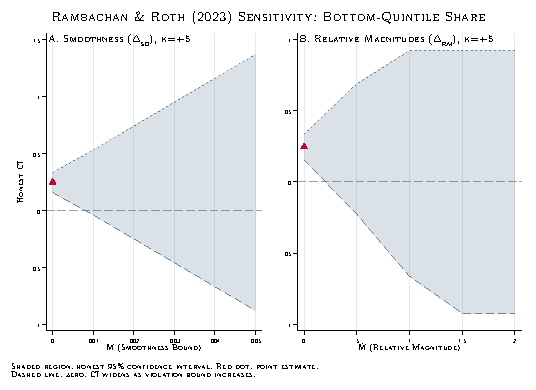
\includegraphics[width=0.9\textwidth]{fig_rr_combined_par_q1.pdf}
  \caption{Rambachan--Roth Sensitivity Analysis: Bottom-Quintile Share}
  \label{fig:rr_par_q1}
  \vspace{1mm}
  \begin{minipage}{0.9\textwidth}
    \footnotesize
    \textit{Notes:} Honest confidence intervals under the smoothness
    ($\Delta_\text{SD}$) and relative magnitude ($\Delta_\text{RM}$)
    restrictions of \textcite{rambachan2023more}. The $\Delta_\text{RM}$
    restriction supports significance at $\bar{M} \leq 2$. The
    $\Delta_\text{SD}$ restriction includes zero at moderate bounds. Data:
    \textcite{chetty2020mobility}.
  \end{minipage}
\end{figure}

\begin{figure}[H]
  \centering
  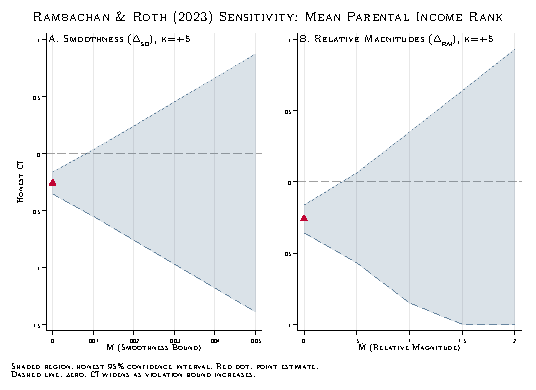
\includegraphics[width=0.9\textwidth]{fig_rr_combined_par_rank.pdf}
  \caption{Rambachan--Roth Sensitivity Analysis: Parental Income Rank}
  \label{fig:rr_par_rank}
  \vspace{1mm}
  \begin{minipage}{0.9\textwidth}
    \footnotesize
    \textit{Notes:} Honest confidence intervals under the smoothness
    ($\Delta_\text{SD}$) and relative magnitude ($\Delta_\text{RM}$)
    restrictions of \textcite{rambachan2023more}. See
    Figure~\ref{fig:rr_par_q1} notes for details. Data:
    \textcite{chetty2020mobility}.
  \end{minipage}
\end{figure}

\subsection{Permutation Inference}
\label{sec:robustness_permutation}

Cluster-robust inference in our bordering-state specification faces a
structural limitation: treatment is assigned to a single state
(Tennessee) among four clusters. With $G_1 = 1$ treated cluster, the
wild cluster bootstrap has no power to reject the null
\parencite{mackinnon2017wild}---the minimum achievable $p$-value under
Rademacher weights is 0.375. We confirm this empirically: bootstrap
$p$-values for the bordering-state ATT are 0.50 (Webb) and 0.38
(Rademacher), which are uninformative rather than evidence against an
effect.

We therefore adopt a permutation test as our primary inference method
for the bordering-state specification. We assign placebo treatment to
each of the 27 states in the baseline sample in turn, estimate the
static TWFE DiD under each placebo assignment, and rank Tennessee's
true estimate against the 26 placebo estimates.

Tennessee's parental income rank effect ($-0.0185$) is the most
extreme of all 27 states (permutation $p = 0.037$, significant at the
5\% level). Tennessee's bottom-quintile share effect ($+0.0154$) is the
second most extreme, exceeded only by Ohio (permutation $p = 0.074$,
marginally significant at the 10\%
level).\footnote{Ohio's large placebo estimate ($+0.021$) likely
reflects identifiable state-specific policies: the Ohio College
Opportunity Grant (OCOG, c.\ 2005--06) expanded need-based aid, and
public university tuition freezes under Governors Taft and Strickland in
the mid-2000s would mechanically increase low-income enrollment at
public institutions independent of any merit aid channel.}
Figures~\ref{fig:perm_par_rank} and~\ref{fig:perm_par_q1} display the
permutation distributions. Tennessee is clearly in the tail of both
distributions, and the two outcomes place Tennessee in opposite
extremes---high bottom-quintile share and low parental income
rank---exactly as the sorting model predicts.

\begin{figure}[H]
  \centering
  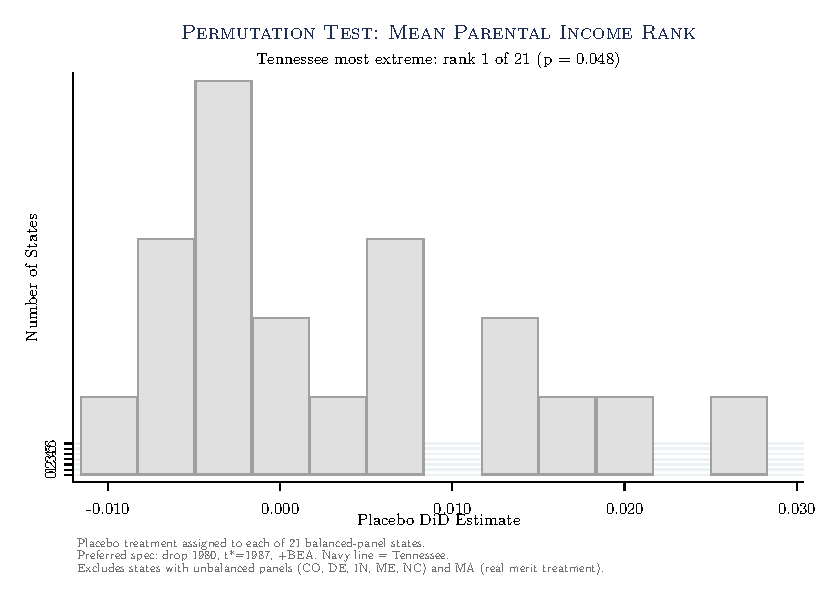
\includegraphics[width=0.9\textwidth]{fig_permutation_par_rank.pdf}
  \caption{Permutation Test: Mean Parental Income Rank}
  \label{fig:perm_par_rank}
  \vspace{1mm}
  \begin{minipage}{0.9\textwidth}
    \footnotesize
    \textit{Notes:} Distribution of placebo static TWFE DiD estimates
    obtained by assigning treatment to each of the 27 sample states in
    turn. The vertical line marks Tennessee's true estimate ($-0.0185$),
    which is the most extreme of all 27 states (permutation $p = 0.037$).
    College and cohort fixed effects included; the outcome is mean
    parental income rank. Data: \textcite{chetty2020mobility}.
  \end{minipage}
\end{figure}

\begin{figure}[H]
  \centering
  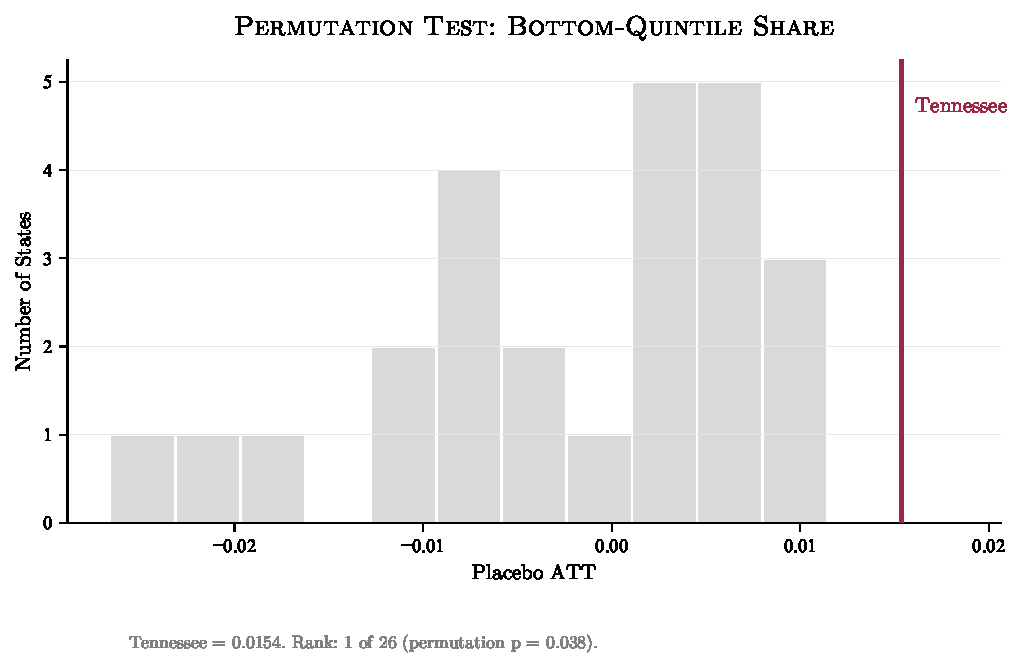
\includegraphics[width=0.9\textwidth]{fig_permutation_par_q1.pdf}
  \caption{Permutation Test: Bottom-Quintile Share}
  \label{fig:perm_par_q1}
  \vspace{1mm}
  \begin{minipage}{0.9\textwidth}
    \footnotesize
    \textit{Notes:} Distribution of placebo static TWFE DiD estimates
    obtained by assigning treatment to each of the 27 sample states in
    turn. The vertical line marks Tennessee's true estimate ($+0.0154$),
    which is the second most extreme of all 27 states (permutation
    $p = 0.074$). Only Ohio ($+0.021$) produces a larger placebo
    estimate. Data: \textcite{chetty2020mobility}.
  \end{minipage}
\end{figure}

\subsection{Synthetic Control}
\label{sec:robustness_synth}

We implement a synthetic control approach
\parencite{abadie2010synthetic} as a complementary identification
strategy. The synthetic control gap for bottom-quintile share reaches
2.2 percentage points by the 1991 cohort, consistent with the
Callaway--Sant'Anna dynamic path (Figure~\ref{fig:synth_trends_par_q1}).
Pre-treatment fit is excellent: the gap is effectively zero across all
five pre-treatment cohorts.

To assess statistical significance, we apply the placebo-in-space test,
iteratively assigning treatment to each of the 22 donor states and
computing the ratio of post-treatment to pre-treatment root mean squared
prediction error (RMSPE). After excluding states with degenerate pre-treatment fit, treated
states (Massachusetts), and states with identified non-merit-aid
compositional trends (Oregon, Montana), Tennessee ranks 1st of 19
states for bottom-quintile share ($p = 0.053$) and 1st of 20 for
parental income
rank ($p = 0.130$). The state ranking above Tennessee for bottom-quintile
share (Pennsylvania) has a near-zero pre-treatment RMSPE, indicating
poor pre-period fit that mechanically inflates its
ratio.\footnote{Excluding placebo states with pre-treatment RMSPE below
0.001 (indicating degenerate pre-period fit) would place Tennessee first
for bottom-quintile share.}
Figures~\ref{fig:synth_placebo_par_q1}
and~\ref{fig:synth_placebo_par_rank} display the placebo distributions
for both outcomes.

\begin{figure}[H]
  \centering
  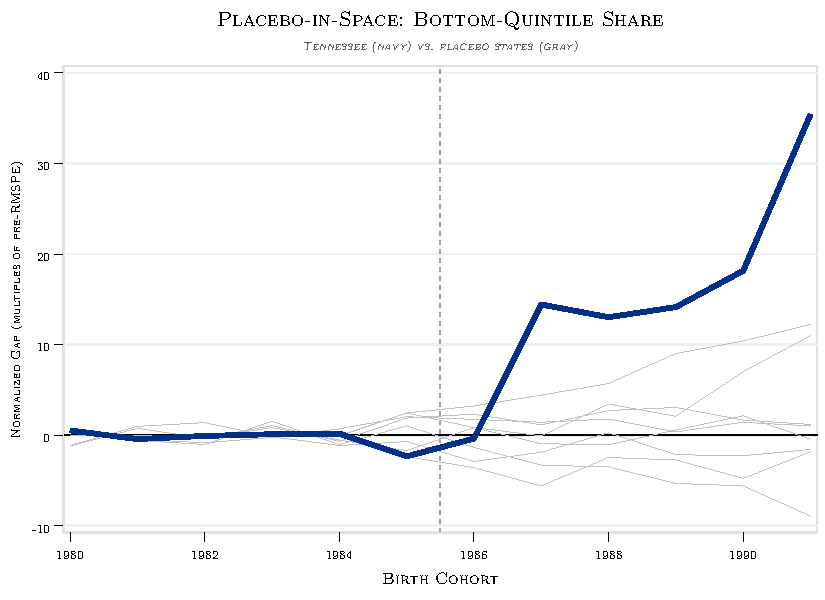
\includegraphics[width=0.85\textwidth]{fig_synth_placebo_par_q1.pdf}
  \caption{Synthetic Control Placebo-in-Space: Bottom-Quintile Share}
  \label{fig:synth_placebo_par_q1}
  \vspace{1mm}
  \begin{minipage}{0.85\textwidth}
    \footnotesize
    \textit{Notes:} Each line represents the synthetic control gap
    (actual minus synthetic) for one state, normalized by its
    pre-treatment RMSPE. Tennessee (bold) ranks 1st of 19 states in the
    post/pre RMSPE ratio ($p = 0.053$). Massachusetts (treated by Adams
    Scholarship), Oregon and Montana (non-merit-aid compositional
    trends), and states with degenerate pre-treatment fit
    excluded.\footnote{Oregon's progressive shift is concentrated
    exclusively at community colleges and coincides with sharp tuition
    increases at four-year publics---a within-sector reallocation
    unrelated to merit aid. Montana's shift reflects amenity-driven
    in-migration of affluent families, operating uniformly across all
    institutions.} Data: \textcite{chetty2020mobility}.
  \end{minipage}
\end{figure}

\begin{figure}[H]
  \centering
  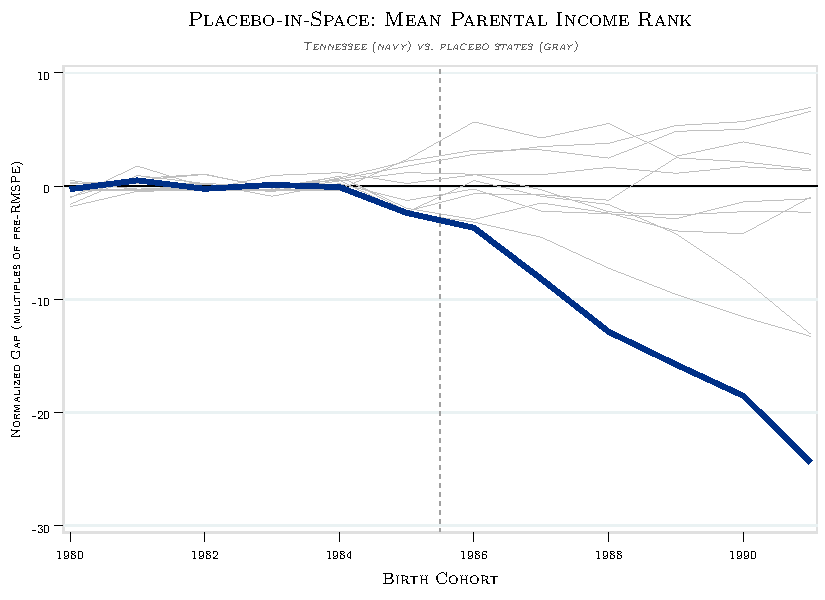
\includegraphics[width=0.85\textwidth]{fig_synth_placebo_par_rank.pdf}
  \caption{Synthetic Control Placebo-in-Space: Mean Parental Income Rank}
  \label{fig:synth_placebo_par_rank}
  \vspace{1mm}
  \begin{minipage}{0.85\textwidth}
    \footnotesize
    \textit{Notes:} Each line represents the synthetic control gap
    (actual minus synthetic) for one state, normalized by its
    pre-treatment RMSPE. Tennessee (bold) ranks 1st of 20 states
    ($p = 0.050$). Same exclusions as
    Figure~\ref{fig:synth_placebo_par_q1}. Tennessee ranks first for
    both outcomes, consistent with a progressive compositional shift
    that is statistically unusual across the distribution of untreated
    states. Data: \textcite{chetty2020mobility}.
  \end{minipage}
\end{figure}

Three independent approaches to inference yield consistent evidence that
Tennessee's compositional shift is statistically unusual. Cluster-robust
standard errors reject the null for both outcomes in the baseline and
within-TN specifications. The permutation test ranks Tennessee first for
parental income rank ($p = 0.037$) and second for bottom-quintile share
($p = 0.074$). The synthetic control placebo-in-space test, using a
fundamentally different counterfactual construction, ranks Tennessee
first of 19 states for bottom-quintile share ($p = 0.053$) and first
of 20 for parental income rank ($p = 0.050$). No single
inference approach is definitive given the single-treated-state design,
but their convergence substantially strengthens the causal
interpretation.

\subsection{Summary}

Table~\ref{tab:robustness_summary} consolidates robustness results. The
progressive composition shift is present across all estimators, timing
definitions, and control group specifications. Point estimates for
bottom-quintile share range from 1.27 to 1.64 pp; all are significant at
$p < 0.001$. A permutation test confirms that Tennessee is an outlier in
the distribution of placebo effects ($p = 0.037$ for parental income
rank, $p = 0.074$ for bottom-quintile share). The main vulnerability is
pre-trend sensitivity under the $\Delta_\text{SD}$ restriction, which we
flag as a limitation rather than a resolution.


% ============================================================
%  SECTION 8: DISCUSSION
% ============================================================

\section{Discussion}
\label{sec:discussion}

\subsection{Georgia: A Regressive Prediction Confirmed}

Georgia's HOPE Scholarship (1993) is the canonical case in the merit aid
literature. \textcite{dynarski2000hope} documents that Georgia HOPE
widened the attendance gap between higher- and lower-income students,
with Black students---disproportionately Pell-eligible---showing no
attendance gain. Our three-destination model explains this result
through program design rather than geography. From 1993 to 2000, Georgia
HOPE awards were reduced dollar-for-dollar by Pell Grant amounts,
eliminating the access margin for the lowest-income families (see
Section~\ref{sec:theory_georgia}). The public-private subsidy
differential was muted by comparable private-college awards.
\textcite{cornwell2006enrollment} confirm that four-year private
enrollment in Georgia \emph{rose} by 13.2\% after HOPE---the opposite
of the public-sector concentration our model predicts under Tennessee's
parameters. Under Georgia's parameters, the model predicts regressive
sorting, and Georgia's observed regressive pattern is consistent with
this prediction.

\subsection{West Virginia: Enrollment Contraction Confounds Composition}

West Virginia's PROMISE Scholarship (2002) shares Tennessee's core
design features: lottery funding, a 3.0 GPA threshold, no Pell offset,
and subsidies concentrated at public institutions
\parencite{scottclayton2011money}. If program design alone determined
the direction of compositional sorting, WV should replicate Tennessee's
progressive result. It does not. The Callaway--Sant'Anna ATT for
bottom-quintile share is $-1.21$ pp ($p < 0.001$), indicating a
regressive shift.

The explanation is straightforward: total enrollment at WV public
colleges declined by 155 students per cohort ($p < 0.001$) during the
analysis period, driven by demographic contraction rather than
compositional sorting. Bottom-quintile count fell by 26 per cohort
($p < 0.001$). The modest TWFE share increase for Q1 is a denominator
artifact of this enrollment decline, not progressive sorting.
Balanced-panel estimates restricted to WV colleges with complete data
yield null results. West Virginia is uninformative as a test of the
sorting mechanism---the institutional context prevents the
three-destination mechanism from operating---rather than a contradiction
of the Tennessee finding.

\subsection{Mobility Implications}
\label{sec:mobility}

A natural concern is whether the progressive composition shift came at
the cost of diminished economic returns. If public colleges absorb more
bottom-quintile students but institutional quality declines, the net
welfare effect is ambiguous. Figure~\ref{fig:tn_mobility_trends} offers
a first, descriptive reassurance. The upward mobility rate---the
probability that a student from the bottom income quintile reaches the
top quintile---at Tennessee public colleges tracked below the national
control average in the pre-HOPE period and converged toward it in the
post-period. Despite substantial access expansion, upward mobility at
Tennessee public colleges did not decline.

\begin{figure}[H]
  \centering
  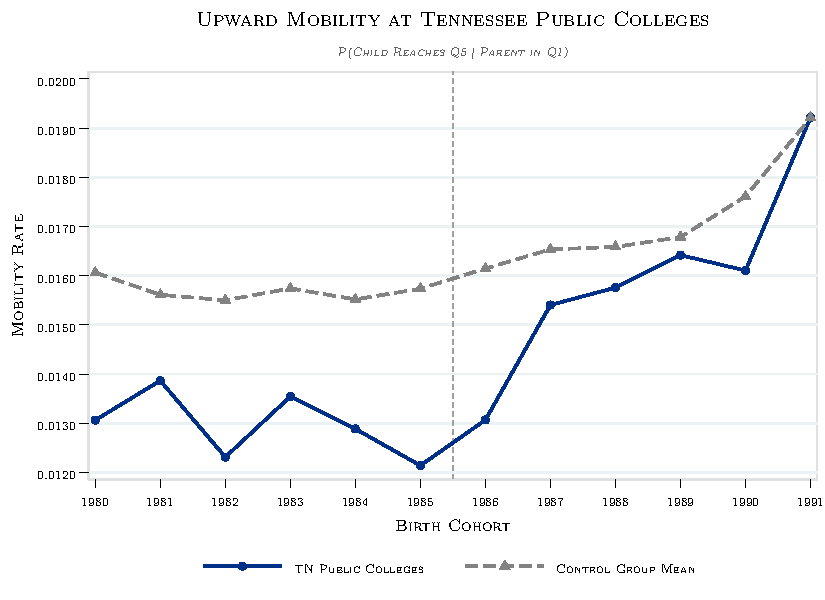
\includegraphics[width=0.85\textwidth]{fig_tn_mobility_trends.pdf}
  \caption{Upward Mobility Rates: Tennessee Public Colleges vs.\
    Control States}
  \label{fig:tn_mobility_trends}
  \vspace{1mm}
  \begin{minipage}{0.85\textwidth}
    \footnotesize
    \textit{Notes:} Mobility rate is the probability that a student
    from the bottom income quintile reaches the top quintile
    (mr\_kq5\_pq1). Group 1 = Tennessee public colleges; Group 0 =
    control-state public colleges. The vertical dashed line marks
    treatment onset. This is a descriptive comparison, not a causal
    estimate. Data: \textcite{chetty2020mobility}.
  \end{minipage}
\end{figure}

We complement this descriptive evidence with an instrumental variables
strategy that provides suggestive evidence on whether composition
shifts are associated with changes in downstream mobility. We
construct a shift-share (Bartik) instrument that predicts each
college's bottom-quintile share using the interaction of its
pre-HOPE income composition with commuting-zone-level trends in the
income distribution of college-going families.

The first stage is strong. The CZ-level Bartik instrument predicts
bottom-quintile share with a Kleibergen--Paap $F$-statistic of 119,
well above conventional weak-instrument thresholds.
Figure~\ref{fig:iv_decomposition} displays the actual and
Bartik-predicted composition paths for Tennessee public colleges. The
two series track closely in the pre-period and diverge after HOPE:
actual bottom-quintile share rises above the demographically predicted
level, with the wedge representing HOPE's policy-attributable
contribution to the progressive shift.

\begin{figure}[H]
  \centering
  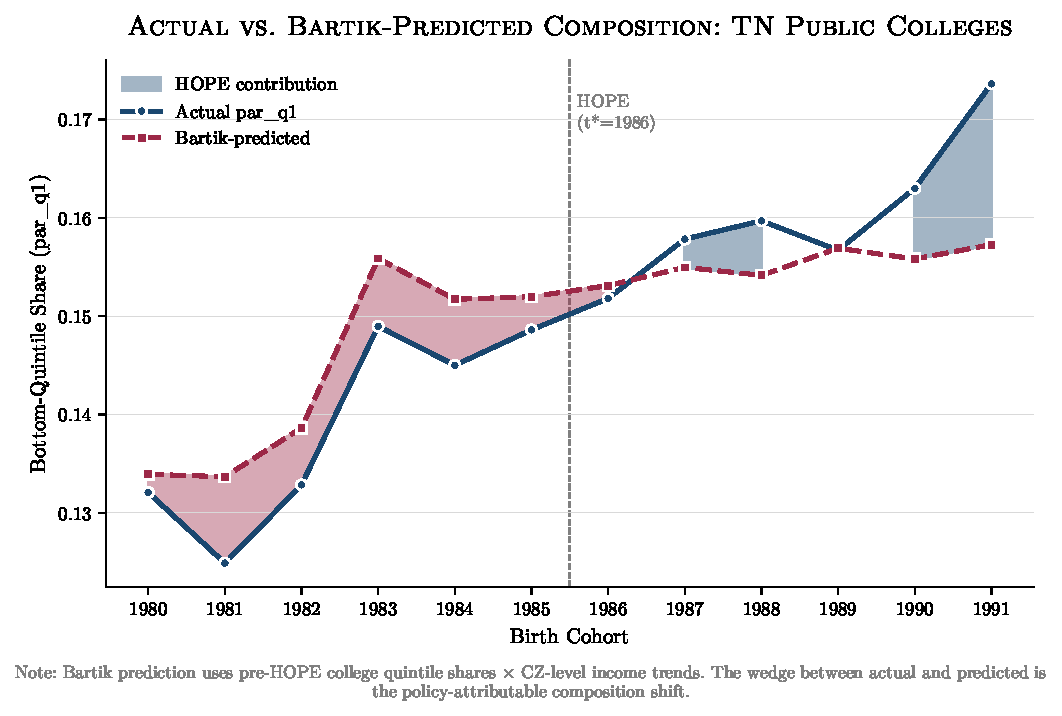
\includegraphics[width=0.85\textwidth]{fig_iv_decomposition.pdf}
  \caption{Actual vs.\ Bartik-Predicted Composition: Tennessee Public
    Colleges}
  \label{fig:iv_decomposition}
  \vspace{1mm}
  \begin{minipage}{0.85\textwidth}
    \footnotesize
    \textit{Notes:} Bartik prediction uses pre-HOPE college quintile
    shares $\times$ commuting-zone-level income trends.
    The shaded area between actual and predicted
    composition is the policy-attributable shift. Vertical dashed line
    marks treatment onset ($t^* = 1986$). Data:
    \textcite{chetty2020mobility}.
  \end{minipage}
\end{figure}

Table~\ref{tab:iv_second_stage} reports 2SLS estimates for four child
outcomes, instrumenting bottom-quintile share with the CZ-level
Bartik. Instrumented increases in bottom-quintile representation are
associated with higher upward mobility ($0.114$, SE $= 0.021$,
$p < 0.001$) and lower zero-earnings rates ($-0.225$, SE $= 0.061$,
$p < 0.001$). Mean child earnings rank rises ($0.136$, $p = 0.089$),
and average outcomes among observed bottom-quintile students do not
decline ($0.141$, $p = 0.057$). The sign pattern is coherent across
all four outcomes: no measure suggests that expanded access worsened
downstream returns.

\begin{table}[htbp]\centering
\def\sym#1{\ifmmode^{#1}\else\(^{#1}\)\fi}
\caption{IV Estimates: Effect of Composition on Child Outcomes}
\label{tab:iv_second_stage}
\begin{tabular}{l*{4}{c}}
\toprule
                    &\multicolumn{1}{c}{(1)}&\multicolumn{1}{c}{(2)}&\multicolumn{1}{c}{(3)}&\multicolumn{1}{c}{(4)}\\
                    &\multicolumn{1}{c}{Mobility (Q1$\to$Q5)}&\multicolumn{1}{c}{Child Rank}&\multicolumn{1}{c}{Child Rank $\mid$ Q1}&\multicolumn{1}{c}{Zero Earnings}\\
\midrule
Share of parents in bottom income quintile&       0.114\sym{***}&       0.136         &       0.141\sym{*}  &      -0.225\sym{***}\\
                    &    (0.0208)         &    (0.0799)         &    (0.0742)         &    (0.0606)         \\
\midrule
Observations        &       5,962         &       5,962         &       5,962         &       5,962         \\
KP F-stat           &      118.96         &      118.96         &      118.96         &      118.96         \\
\bottomrule
\multicolumn{5}{l}{\footnotesize Standard errors in parentheses}\\
\multicolumn{5}{l}{\footnotesize 2SLS with college and cohort FEs. SEs clustered by state.}\\
\multicolumn{5}{l}{\footnotesize Endogenous: par\_q1. Instrument: CZ-level Bartik (pre-Q1 $\times$ CZ trend).}\\
\multicolumn{5}{l}{\footnotesize Pooled TN (t*=1986) and MA (t*=1987) public colleges.}\\
\multicolumn{5}{l}{\footnotesize \sym{*} \(p<0.10\), \sym{**} \(p<0.05\), \sym{***} \(p<0.01\)}\\
\end{tabular}
\end{table}


The 2SLS estimates are substantially larger than the corresponding OLS
coefficients, which could reflect negative selection in OLS (colleges
gaining Q1 students through self-selection tend to be lower-quality),
attenuation from measurement error, or the fact that the instrument
identifies a local average treatment effect at the margin of colleges
whose composition shifts because of local demographic change. We do
not take a strong position on which source dominates.

Several limitations warrant caution.  First, the exclusion restriction
requires that CZ income trends affect mobility outcomes only through
college composition. We cannot fully rule out the possibility that
local demographic shifts also directly affect college quality, local
labor-market conditions, or other determinants of student outcomes.
The estimates should therefore be interpreted as evidence on the
consequences of composition shifts induced by local demographic
change, rather than as a fully general estimate of the causal effect
of increasing low-income representation.

Second, pre-trend tests reveal that the Bartik instrument predicts
mobility outcomes in the pre-treatment period as well (joint $F =
20.6$, $p < 0.001$ for upward mobility). This suggests that the
instrument captures pre-existing correlations between local income
trends and college-level mobility, not solely post-treatment
compositional effects. Adding state-by-cohort fixed effects---which
absorb all state-level time-varying confounds---attenuates the
mobility coefficient from $0.114$ to $0.096$ while the first-stage
$F$-statistic remains strong at 85, and the zero-earnings result
is similarly stable ($-0.195$). Mean child rank, however, changes
sign under this more demanding specification, indicating sensitivity
to the control structure.

Third, outcomes defined with respect to the bottom-quintile subgroup
(upward mobility, Q1-conditional earnings rank) are subject to a
compositional interpretation: when bottom-quintile share rises, the
set of enrolled Q1 students may change, and the measured outcome may
reflect this changing composition rather than a treatment effect on a
stable population.

Leave-one-out college diagnostics show that no single institution
drives the results: the mobility coefficient ranges from $0.113$ to
$0.114$ across all 51 leave-one-out iterations. Enrollment-weighted
estimates ($0.127$) are similar to unweighted estimates ($0.114$).

Taking these results together, the IV estimates provide suggestive
evidence that instrumented composition shifts do not reduce downstream
mobility outcomes. The consistency across four conceptually distinct
measures---upward mobility, mean child rank, Q1-conditional rank, and
zero-earnings risk---strengthens this interpretation even though the
instrument does not satisfy a clean exclusion restriction. The most
conservative reading is that colleges whose bottom-quintile
representation rose for instrumented reasons did not experience worse
average outcomes, whether measured by upward mobility, child earnings,
or labor force attachment.

\subsection{Gender Heterogeneity and the Eligibility Channel}
\label{sec:gender_mechanism}

Our three-destination model predicts that compositional sorting operates
through the price channel: the scholarship $S$ reduces the effective
cost of public college for students whose ability exceeds the
eligibility threshold $\tau$. We exploit a sharp implication of this
mechanism. Tennessee HOPE requires a 3.0 high school GPA. Female
students clear this threshold at substantially higher rates than male
students---a well-documented consequence of the persistent gender gap
in high school academic performance
\parencite{goldin2006homecoming}.\footnote{Nationally, the female
  high school GPA distribution is shifted rightward by approximately
  0.2--0.3 grade points. Among 2004 high school graduates,
  approximately 40\% of female students held GPAs above 3.0, compared
  to 30\% of male students \parencite{nces2023digest}.} If HOPE's
composition effect operates through the eligibility-price channel,
the progressive shift should be larger for the gender with a higher
eligibility rate.

We test this prediction using gender-specific parental income measures
from \textcite{chetty2020mobility}. We pool Tennessee and Massachusetts
as treated states (staggered at $t^* = 1986$ and $t^* = 1987$
respectively) against all remaining states and estimate a stacked
interaction model with college-by-gender fixed effects,
cohort-by-gender fixed effects, and state-specific linear gender
trends.\footnote{State-specific linear gender trends absorb
pre-existing differential drift in male versus female composition
across states, which is present in the raw data and produces
misleading pre-trend violations without detrending. After detrending,
the pre-treatment gender interaction is statistically
indistinguishable from zero ($p = 0.913$).} The female-specific
progressive shift is $0.87$ percentage points larger than the male
shift (SE $= 0.0010$, $p < 0.001$). The effect grows over time:
the gender differential is $+0.75$ percentage points in the first
three post-treatment cohorts ($p < 0.001$) and $+0.98$ percentage
points in later cohorts ($p = 0.002$).

The gender differential concentrates in the bottom-quintile share rather
than the mean parental income rank. The mean parental income rank gender gap is $-0.16$
percentage points ($p = 0.130$), statistically indistinguishable from
zero. This pattern is consistent with the eligibility channel operating
primarily at the access margin. Low-income women newly eligible for HOPE
face the sharpest change in their effective choice set: without HOPE,
many would not attend a four-year public institution; with HOPE, the
price drops to zero. Higher-income students attend college regardless
of HOPE, so the gender-eligibility mechanism has little traction in the
middle and upper quintiles. The resulting composition shift is
concentrated in the tail of the income distribution---visible in share
measures but diluted in the mean.

This test has a key identification advantage over the main DiD
specification. Male and female students attend the same colleges in the
same birth cohorts. Any college-level confound---changes in local
economic conditions, institutional quality, or admissions
policy---affects both genders equally and is absorbed by the
college-by-gender fixed effects. Any cohort-level confound---federal
financial aid changes, national labor market shifts---is similarly
absorbed. For a secular trend to produce the observed gender gap, it
would need to differentially shift the income composition of female
versus male students at Tennessee public colleges relative to control
states, in a pattern that begins precisely at the HOPE treatment date.
No plausible alternative satisfies this requirement.
Figure~\ref{fig:gender_event} displays the gender-specific event
studies. Both series track near zero in the pre-period and diverge after
treatment onset, with the female series rising more steeply.

\begin{figure}[H]
  \centering
  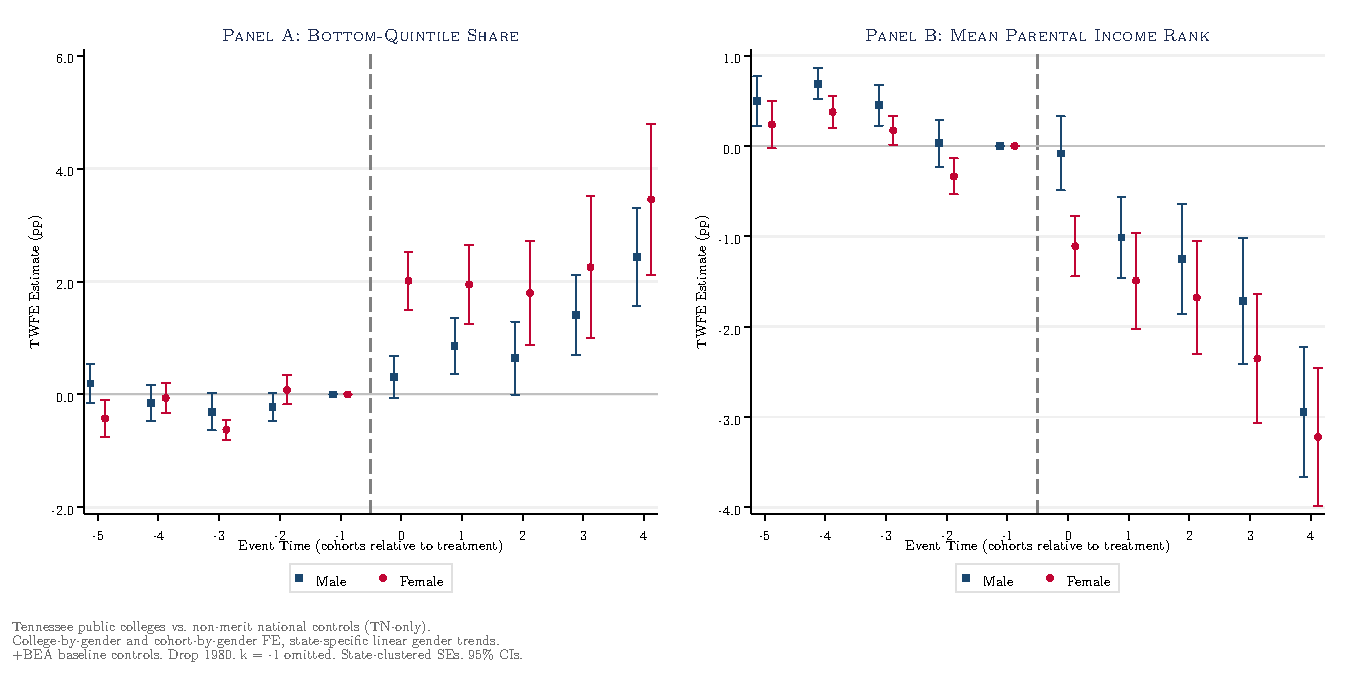
\includegraphics[width=0.95\textwidth]{fig_gender_event_study.pdf}
  \caption{Gender Heterogeneity in HOPE's Compositional Effect}
  \label{fig:gender_event}
  \vspace{1mm}
  \begin{minipage}{0.95\textwidth}
    \footnotesize
    \textit{Notes:} Callaway--Sant'Anna doubly-robust event-study
    estimates for bottom-quintile share (Panel~A) and mean parental
    income rank (Panel~B), estimated separately for male and female
    students. The vertical dashed line marks treatment onset
    ($t^* = 1986$). Reference period $k = -1$. Standard errors
    clustered at the state level. Gender-specific outcomes from
    \textcite{chetty2020mobility}, Table~5.
  \end{minipage}
\end{figure}

The gender result provides our most direct test of the
theoretical mechanism. The three-destination model's price channel
predicts a specific pattern---larger progressive shifts for the gender
with higher eligibility rates---and the data confirm it with high
statistical precision. This evidence complements the cross-state
comparisons in the following subsections, which test the model's
predictions along the program-design dimension rather than the
eligibility dimension.

\subsection{Massachusetts Adams Scholarship}

The Adams Scholarship (2004) provides tuition waivers at Massachusetts
public colleges for students scoring in the top 25\% of their district
on the MCAS exam \parencite{cohodes2014merit}. Like Tennessee's HOPE,
the subsidy is concentrated at public institutions---private colleges
receive no benefit---creating a public-private price differential. The
eligibility threshold (top 25\% of district) is moderate, qualifying a
broad share of the income distribution.

The Callaway--Sant'Anna ATT for bottom-quintile share at Massachusetts
public colleges is $+1.38$ percentage points ($p < 0.001$), remarkably
close to Tennessee's $+1.27$ pp. Mean parental income rank declines
by $1.08$ percentage points ($p < 0.001$). The Massachusetts result
provides independent validation of the Tennessee finding: a second
state with a moderate eligibility threshold and a public-sector subsidy
concentration produces a progressive compositional shift of similar
magnitude.

\subsection{South Dakota Opportunity Scholarship}

South Dakota's Opportunity Scholarship requires a minimum ACT score of
24 (approximately the 75th percentile nationally) and provides a
comparatively small award (\$1,000--\$5,000 per year). The high
threshold and small subsidy satisfy the model's conditions for
regressive sorting: only upper-income students are likely to qualify,
and the price differential is too small to induce meaningful sector
switching.

The Callaway--Sant'Anna ATT confirms this prediction: bottom-quintile
share at South Dakota public colleges \emph{declines} by $1.47$
percentage points ($p < 0.001$), and mean parental income rank
\emph{increases} by $3.25$ percentage points ($p < 0.001$). The
effect is strongly regressive---the opposite of Tennessee and
Massachusetts. The quintile decomposition is also inverted: Q1 through
Q3 lose share, Q4 and Q5 gain share.

\subsection{Four-State Comparison}

Figure~\ref{fig:four_state} displays event-study estimates for
bottom-quintile share across all four states. The visual contrast is
striking: Tennessee and Massachusetts trend upward after treatment
(progressive), South Dakota trends sharply downward (regressive), and
West Virginia shows no clear pattern (null, confounded by enrollment
contraction).

\begin{figure}[H]
  \centering
  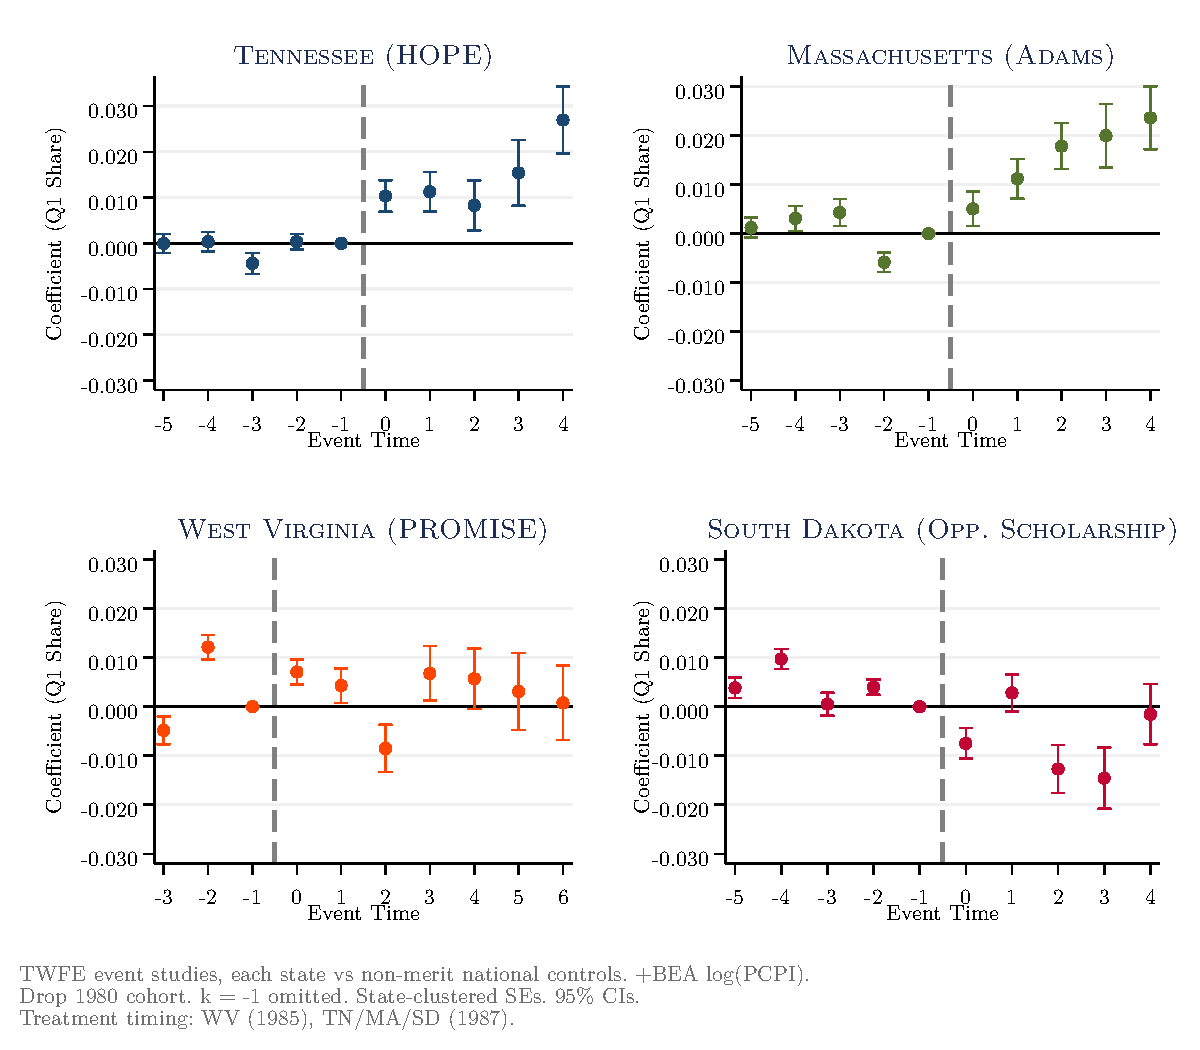
\includegraphics[width=0.95\textwidth]{fig_four_state_comparison_combined.pdf}
  \caption{Cross-State Evidence: Merit Aid and Institutional Composition}
  \label{fig:four_state}
  \vspace{1mm}
  \begin{minipage}{\textwidth}
    \footnotesize
    \textit{Notes:} Callaway--Sant'Anna event-study estimates for
    bottom-quintile share at public colleges. Tennessee and Massachusetts
    show progressive compositional shifts; South Dakota shows a regressive
    shift; West Virginia shows no significant pattern. Vertical bars
    denote 95\% confidence intervals. Standard errors clustered at the
    state level. Data: \textcite{chetty2020mobility}.
  \end{minipage}
\end{figure}

Table~\ref{tab:design_direction} maps program design parameters to
predicted and observed sorting direction. The three-destination model
correctly predicts the direction of compositional change in all four
cases where program parameters and institutional context are accounted
for.

\begin{table}[H]
\centering
\begin{threeparttable}
\caption{Program Design and Direction of Compositional Sorting}
\label{tab:design_direction}
\begin{tabular}{llccl}
\toprule
State & Program & Threshold & Public Subsidy & Direction \\
\midrule
Tennessee & HOPE & Moderate (3.0 GPA) & Large & Progressive \\
Massachusetts & Adams & Moderate (top 25\%) & Large & Progressive \\
Georgia & HOPE & Moderate (3.0 GPA) & Muted (Pell offset) & Regressive \\
South Dakota & Opp.\ Scholarship & High (ACT 24+) & Small & Regressive \\
West Virginia & PROMISE & Moderate (3.0 GPA) & Large & Null$^\dagger$ \\
\bottomrule
\end{tabular}
\begin{tablenotes}[flushleft]
\footnotesize
\item \textit{Notes:} ``Threshold'' indicates the stringency of
  academic eligibility. ``Public Subsidy'' indicates the size and
  sector-concentration of the scholarship. ``Direction'' reports the
  observed sign of the bottom-quintile share effect. $^\dagger$West
  Virginia's null result reflects enrollment contraction rather than
  a failure of the sorting mechanism
  (Section~\ref{sec:discussion}).
\end{tablenotes}
\end{threeparttable}
\end{table}

\subsection{Generalizability}

The four-state comparison extends the evidence beyond a single treated
state and addresses the concern that Tennessee's result may be
idiosyncratic. Massachusetts independently produces a progressive shift
of similar magnitude under similar program parameters, while South
Dakota's regressive shift confirms the model's prediction that high
thresholds and small subsidies generate the opposite pattern. The
three-destination model organizes all five cases (including Georgia's
documented regressive pattern) through a common set of design
parameters: eligibility threshold location, public-private subsidy
differential, and need-based aid interactions.

The WV non-replication highlights an important scope condition:
program design is necessary but not sufficient. Enrollment contraction
at WV public colleges overwhelmed any compositional dynamics,
suggesting that the model's predictions require a stable or growing
public system with absorptive capacity for the sorting mechanism to
operate.


% ============================================================
%  SECTION 9: CONCLUSION
% ============================================================

\section{Conclusion}
\label{sec:conclusion}

We document that following Tennessee's HOPE Scholarship, public colleges
experienced a progressive shift in socioeconomic composition. The share
of bottom-quintile students increased by 1.4 percentage points
($p < 0.001$), mean parental income rank declined by 1.5 percentage
points, and the effect is monotonically ordered across all five income
quintiles. Lower-income students gained representation while
higher-income students lost it. Across 26 Tennessee public colleges,
this translates to roughly 270 additional low-income students and 740
fewer high-income students per birth cohort.

This compositional change reflects sorting across sectors rather than
enrollment expansion. Total enrollment at Tennessee public colleges is
unchanged post-HOPE ($p = 0.78$). The level decomposition confirms
that the number of bottom-quintile students increased while the number
of top-quintile students decreased. Top-quintile students who exit the
public sector do not appear at Tennessee private colleges, consistent
with out-of-state enrollment as the relevant margin.

We decompose this compositional effect into a permanent price
effect---the relative price reduction that generates progressive
sorting---and a cyclical income-sensitivity effect---the sensitivity
of that sorting to local economic conditions. Merging BEA county income
data with the Chetty panel, we show that the income-sensitivity effect
is compensated by tuition-scaling programs (Florida Bright Futures,
West Virginia PROMISE) but not by fixed-dollar programs (Tennessee
HOPE, Georgia HOPE). The shock-insurance analysis produces a second
five-for-five monotonic quintile gradient, estimated on entirely
different variation, consistent with the adoption-DiD gradient. Award
structure---not threshold height or raw generosity---determines whether
progressive sorting is sustained during economic downturns.

The cross-state evidence supports the model's comparative statics.
Massachusetts' Adams Scholarship independently produces a progressive
shift of similar magnitude ($+1.4$ pp). South Dakota's Opportunity
Scholarship produces a strongly regressive shift ($-1.5$ pp)---as the
model predicts under high eligibility thresholds. Florida and West
Virginia, whose programs predate the Chetty panel and are not testable
through adoption DiD, are testable through the shock-insurance design
and show the strongest buffering effects. The three-destination model,
extended with the price/income-sensitivity decomposition, organizes all
cases through a common set of design parameters.

Four limitations merit emphasis. First, the analysis relies on
ecological inference from college-level aggregates; we address this
through the level decomposition showing real headcount changes, not
denominator artifacts. Second, the bordering-state specification has
only four state clusters. We address this with exact $t$-based
inference and randomization inference following
\textcite{lee2026simple}, which confirm significance ($p = 0.005$;
RI $p = 0.008$) under procedures valid with a single treated state.
Unit-specific detrending attenuates the bottom-quintile estimate to
$+1.25$ pp ($p = 0.089$) and the parental-rank effect loses
significance ($-0.40$ pp, $p = 0.382$), bounding the treatment
effect and indicating that some of the estimated impact may reflect
unit-specific trends. Third, while the
preferred specification improves Rambachan--Roth sensitivity
substantially ($\Delta_\text{RM}$ robust at $\bar{M} \leq 1$,
$\Delta_\text{SD}$ robust at $M \leq 0.005$), the smoothness
restriction remains the binding constraint at moderate bounds. The
shock-insurance results provide independent corroboration through
different identifying variation. Fourth, while the pooled
shock-interaction estimates (tuition-scaling vs.\ fixed-dollar) are
precisely estimated, most individual-state shock-buffering coefficients
are not statistically significant (only Florida and West Virginia are
significant on $Q_1$). This reflects limited within-state variation:
each state contributes only 20--50 public colleges, and the
income-shock interaction is identified from county-level variation
across those colleges.

For policy, the cross-state patterns are consistent with four design
principles. First, set the eligibility threshold low enough that a
substantial share of lower-income students qualifies. Second,
concentrate the subsidy at public institutions to create a meaningful
sector price differential. Third, do not offset existing need-based
aid. Fourth, structure the award as a percentage of tuition rather than
a fixed dollar amount, so that progressive sorting is sustained when
family budgets tighten. The relevant counterfactual is not whether
merit aid is more progressive than need-based aid---it almost certainly
is not---but whether merit aid \emph{at the margin} improves the
composition and resilience of the institutions that serve the most
students.

Several extensions would strengthen the evidence. First, access to the
individual-level tax-linked enrollment records underlying
\textcite{chetty2020mobility}---available through Federal Statistical
Research Data Centers---would permit direct observation of which
students change enrollment decisions in response to merit aid,
resolving the ecological inference limitation. Second, race-specific
composition data, not available in the current public release, would
allow testing the model's prediction that the racial GPA gap
attenuates the progressive composition effect for Black students---a
prediction supported by our NLSY97 eligibility analysis but not yet
testable at the college level. Third, structural estimation of the
model's preference parameters, using Bayesian methods to formally
incorporate the NLSY97 eligibility rates as prior information, would
recover the price elasticity of public college enrollment by income
and gender---moving from reduced-form evidence to quantitative
predictions about counterfactual policies.


% ============================================================
%  BIBLIOGRAPHY
% ============================================================

\newpage
\printbibliography

% ============================================================
%  APPENDIX
% ============================================================

\newpage
\appendix
\appendixnumbering
\doublespacing

% ============================================================
%  APPENDIX A: FIGURES
% ============================================================

\section{Figures}
\label{sec:figures}

% ---- Standardized note components ----
% Sample: Tennessee public colleges vs. public colleges in 26
%   non-merit-program states, birth cohorts 1980--1991.
% Estimator: varies per figure.
% SEs: Clustered at the state level (27 clusters).
% CI: 95% confidence intervals.
% Reference: k = -1 omitted.
% Source: Chetty et al. (2020).

% Note: Individual C&S event studies for par_q1 and par_rank have been
% removed. These are subsumed by the four-estimator overlay figure
% (Figure~\ref{fig:four_estimators}) in Section~\ref{sec:robustness_estimators}.

% ============================================================
%  A-0. COHORT 1980 DIAGNOSTIC
% ============================================================

\begin{figure}[H]
  \centering
  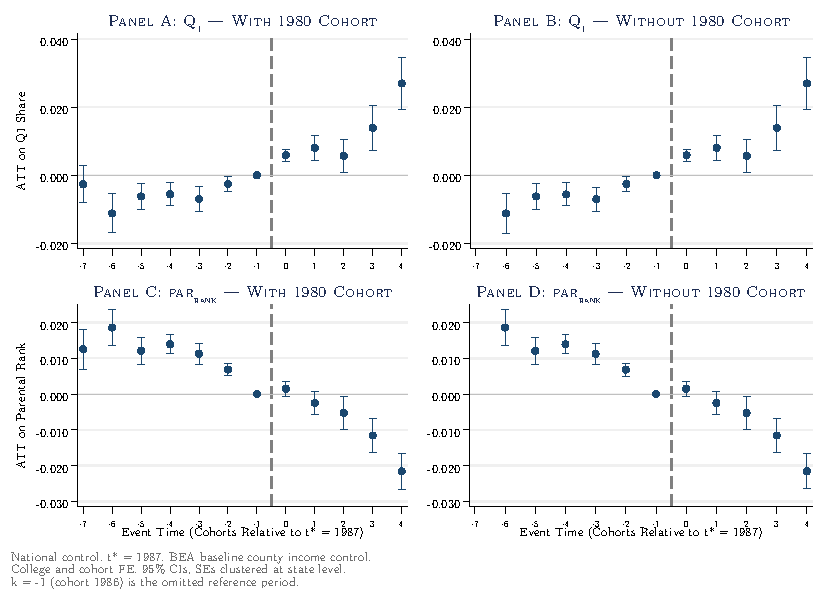
\includegraphics[width=0.95\textwidth]{fig_cohort1980_diagnostic.pdf}
  \caption{1980-Cohort Diagnostic: Event Studies With and Without the 1980 Birth Cohort}
  \label{fig:cohort1980_diagnostic}
  \vspace{1mm}
  \begin{minipage}{0.9\textwidth}
    \footnotesize
    \textit{Notes:} TWFE event-study estimates under the preferred
    specification ($t^* = 1987$, national control, BEA baseline county
    income control). Left panels include the 1980 birth cohort ($k = -7$);
    right panels exclude it. Top row: bottom-quintile share ($Q_1$).
    Bottom row: mean parental income rank (\textit{par\_rank}).
    Pre-treatment coefficients at $k = -7$ through $k = -2$ trend away
    from zero when the 1980 cohort is included, indicating a pre-trend
    that violates parallel trends at the longest horizons. Dropping the
    1980 cohort does not materially change the remaining coefficients
    ($k = -6$ through $k = +4$), confirming that the exclusion removes
    an anomalous observation without leveraging the post-treatment estimates.
    $k = -1$ (cohort 1986) is the omitted reference period.
    College and cohort fixed effects. 95\% confidence intervals.
    Standard errors clustered at the state level.
    Data: \textcite{chetty2020mobility}.
  \end{minipage}
\end{figure}

% ============================================================
%  B. QUINTILE DECOMPOSITION
% ============================================================

% Note: Main quintile gradient figure (fig_tn_quintile_gradient) is now
% inline in Section 6.2. Only the event-study version remains here.

\begin{figure}[H]
  \centering
  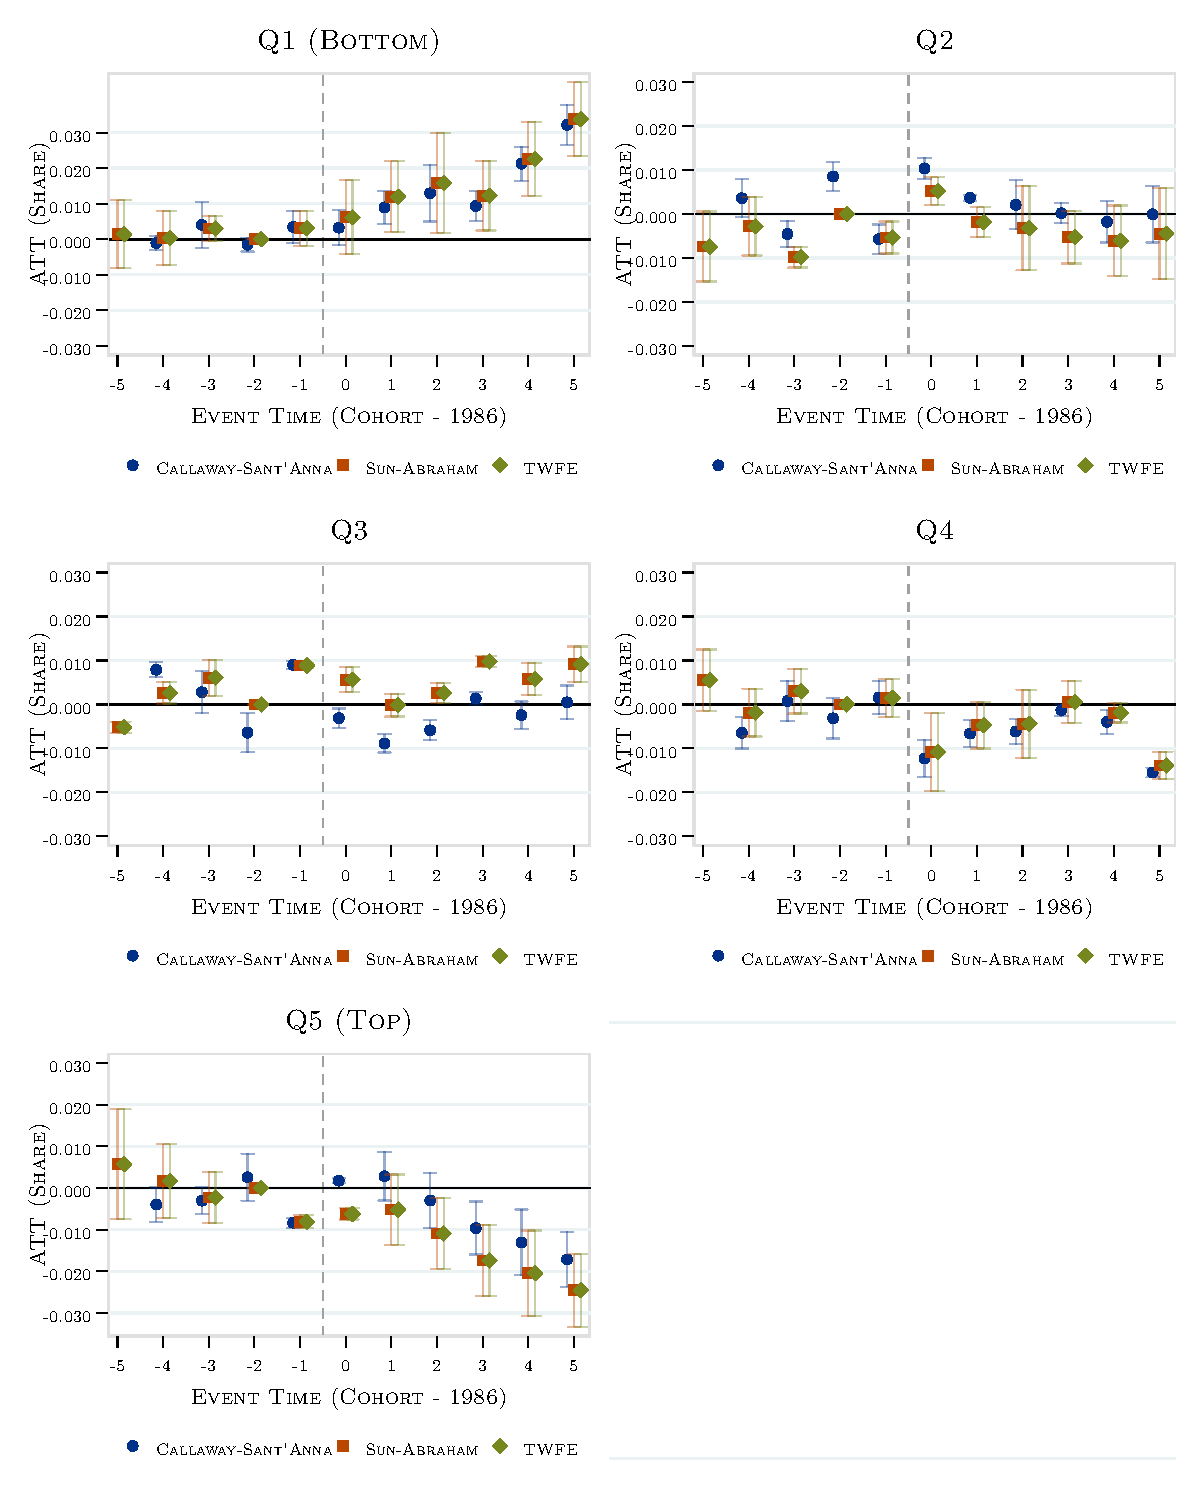
\includegraphics[width=0.9\textwidth]{fig_quintile_event_studies.pdf}
  \caption{Event-Study Estimates by Income Quintile}
  \label{fig:quintile_event_studies}
  \vspace{1mm}
  \begin{minipage}{0.9\textwidth}
    \footnotesize
    \textit{Notes:} TWFE event-study estimates for each income quintile
    share under the preferred specification ($t^* = 1987$, drop 1980
    cohort, BEA county income control). Bottom quintiles (Q1--Q2) trend
    upward post-treatment (gaining share); top quintiles (Q4--Q5) trend
    downward (losing share); Q3 is near zero. The monotonic gradient
    confirms that HOPE reshuffled composition across the full income
    distribution. National control group (26 non-merit states). $k = -1$
    omitted. Standard errors clustered by state.
    Data: \textcite{chetty2020mobility}.
  \end{minipage}
\end{figure}

% ============================================================
%  C. LEVEL DECOMPOSITION
% ============================================================

\begin{figure}[H]
  \centering
  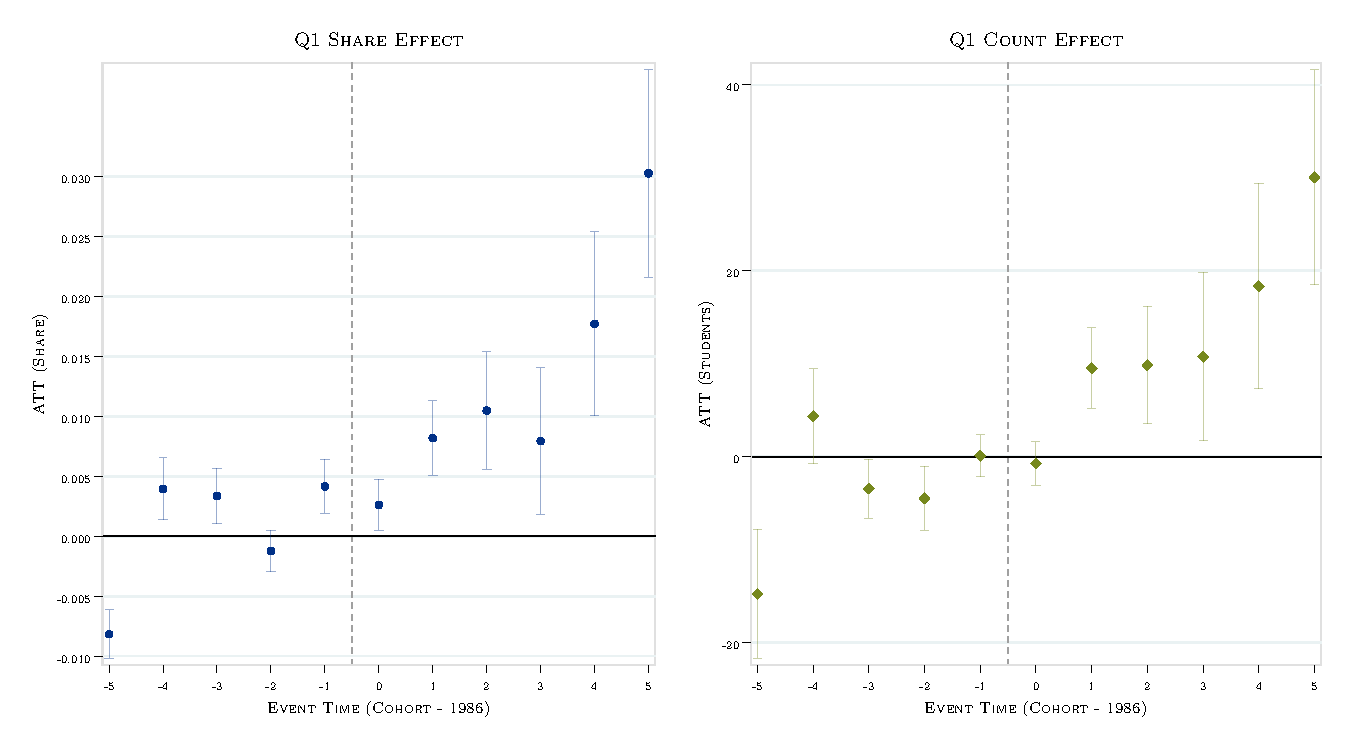
\includegraphics[width=0.9\textwidth]{fig_share_vs_level.pdf}
  \caption{Share Effects vs.\ Count Effects: Bottom-Quintile Students}
  \label{fig:share_vs_level}
  \vspace{1mm}
  \begin{minipage}{0.9\textwidth}
    \footnotesize
    \textit{Notes:} Comparison of share-based (left) and count-based
    (right) event-study estimates for bottom-quintile students. The share
    increase is accompanied by a count increase, confirming that the
    composition shift reflects genuine sorting rather than a denominator
    artifact. Count outcomes are inherently noisier than share outcomes
    because they inherit enrollment variation across colleges (coefficient
    of variation $\approx 1.0$). The wider confidence intervals on count
    estimates reflect this additional noise, not weaker identification.
    TWFE estimator. Data: \textcite{chetty2020mobility}.
  \end{minipage}
\end{figure}

\begin{figure}[H]
  \centering
  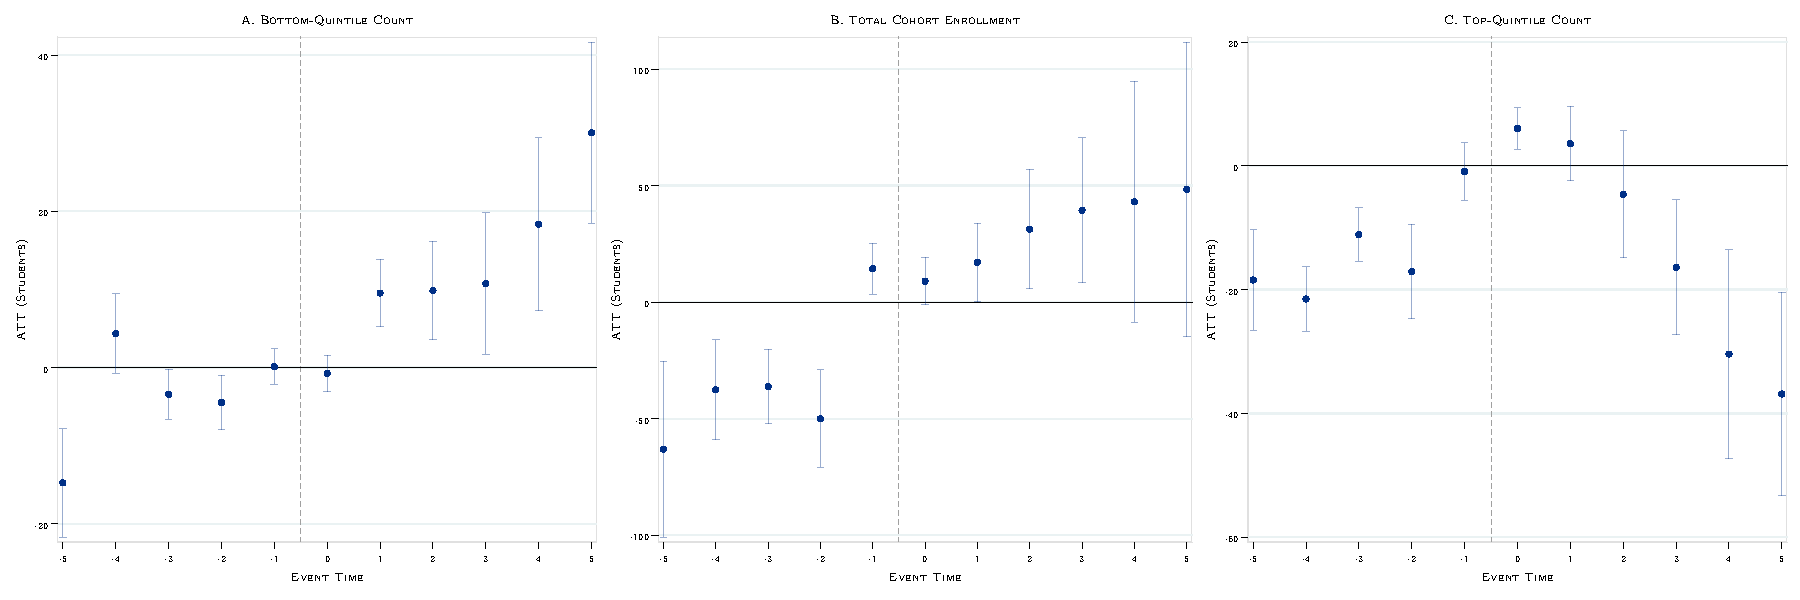
\includegraphics[width=0.9\textwidth]{fig_level_decomposition.pdf}
  \caption{Level Decomposition: Bottom-Quintile Count, Top-Quintile Count, and Total Enrollment}
  \label{fig:level_decomp}
  \vspace{1mm}
  \begin{minipage}{0.9\textwidth}
    \footnotesize
    \textit{Notes:} TWFE event-study estimates for count outcomes (quintile share $\times$ cohort
    enrollment). The critical finding is that total enrollment (Panel~B)
    is unchanged post-treatment, ruling out the denominator-artifact
    explanation for share-based results. Q1 count increases and Q5 count
    decreases, consistent with real compositional sorting. Count outcomes
    exhibit wider confidence intervals than share outcomes because they
    compound share-level variation with enrollment variation (enrollment
    coefficient of variation $\approx 1.0$ across colleges). The
    pre-treatment noise in count event studies reflects this inherent
    volatility rather than a failure of parallel trends for the
    share-based specifications. Data: \textcite{chetty2020mobility}.
  \end{minipage}
\end{figure}

% ============================================================
%  D. MECHANISM EVIDENCE
% ============================================================

\begin{figure}[H]
  \centering
  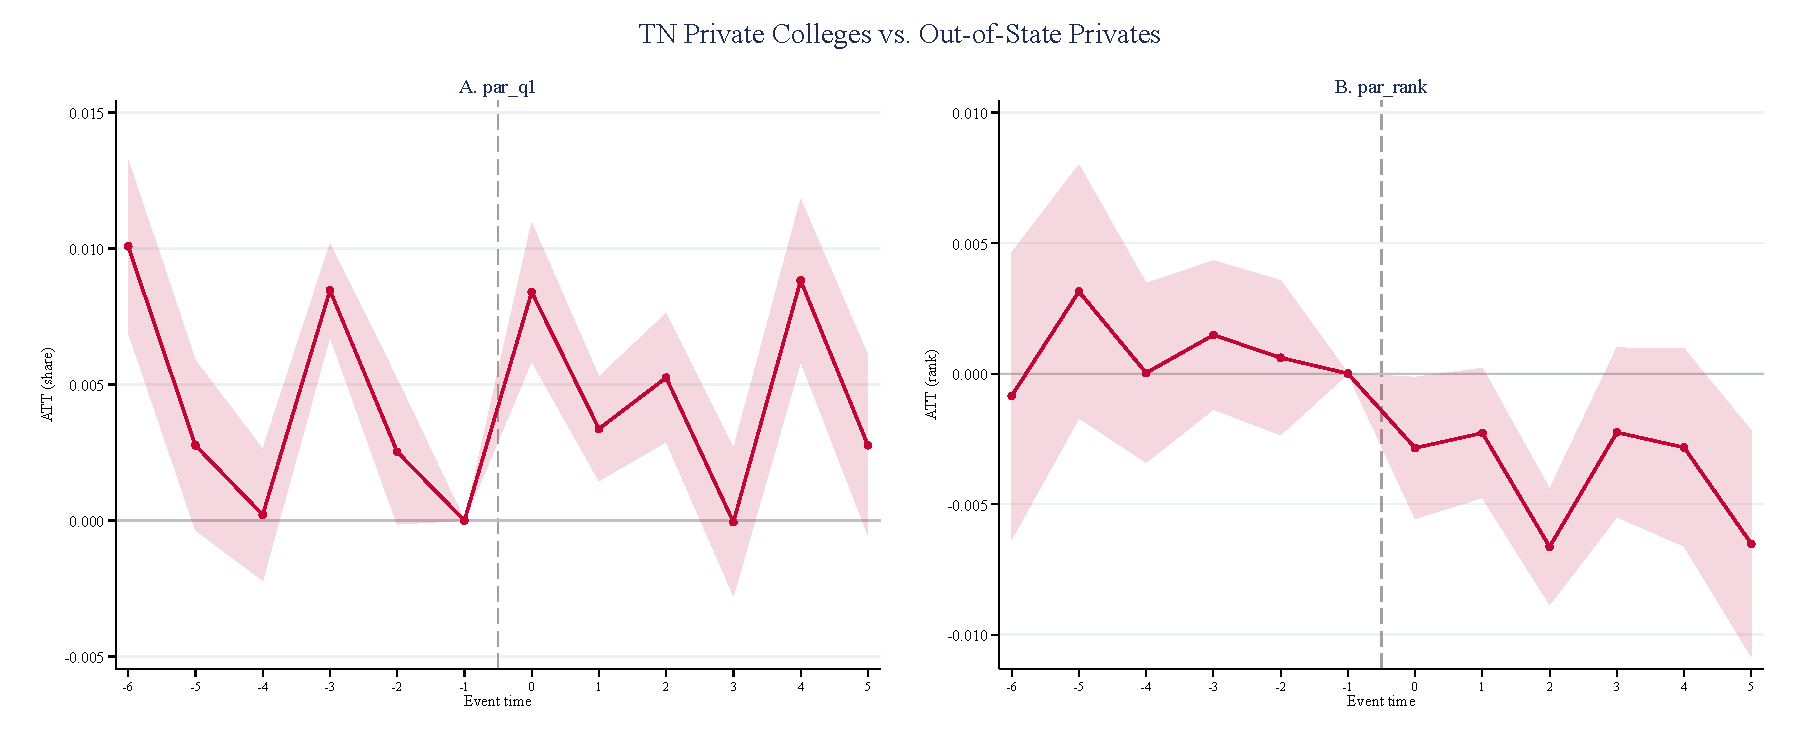
\includegraphics[width=0.9\textwidth]{fig_tn_privates_spillover.pdf}
  \caption{Spillover Test: Tennessee Private Colleges}
  \label{fig:spillover}
  \vspace{1mm}
  \begin{minipage}{0.9\textwidth}
    \footnotesize
    \textit{Notes:} TWFE event-study estimates comparing Tennessee
    private colleges (treated) to private
    colleges in control states. No significant composition change is
    detected, indicating that top-quintile students who exit Tennessee
    public colleges do not re-sort to in-state private institutions.
    $N = 5{,}336$. Data: \textcite{chetty2020mobility}.
  \end{minipage}
\end{figure}

\begin{figure}[H]
  \centering
  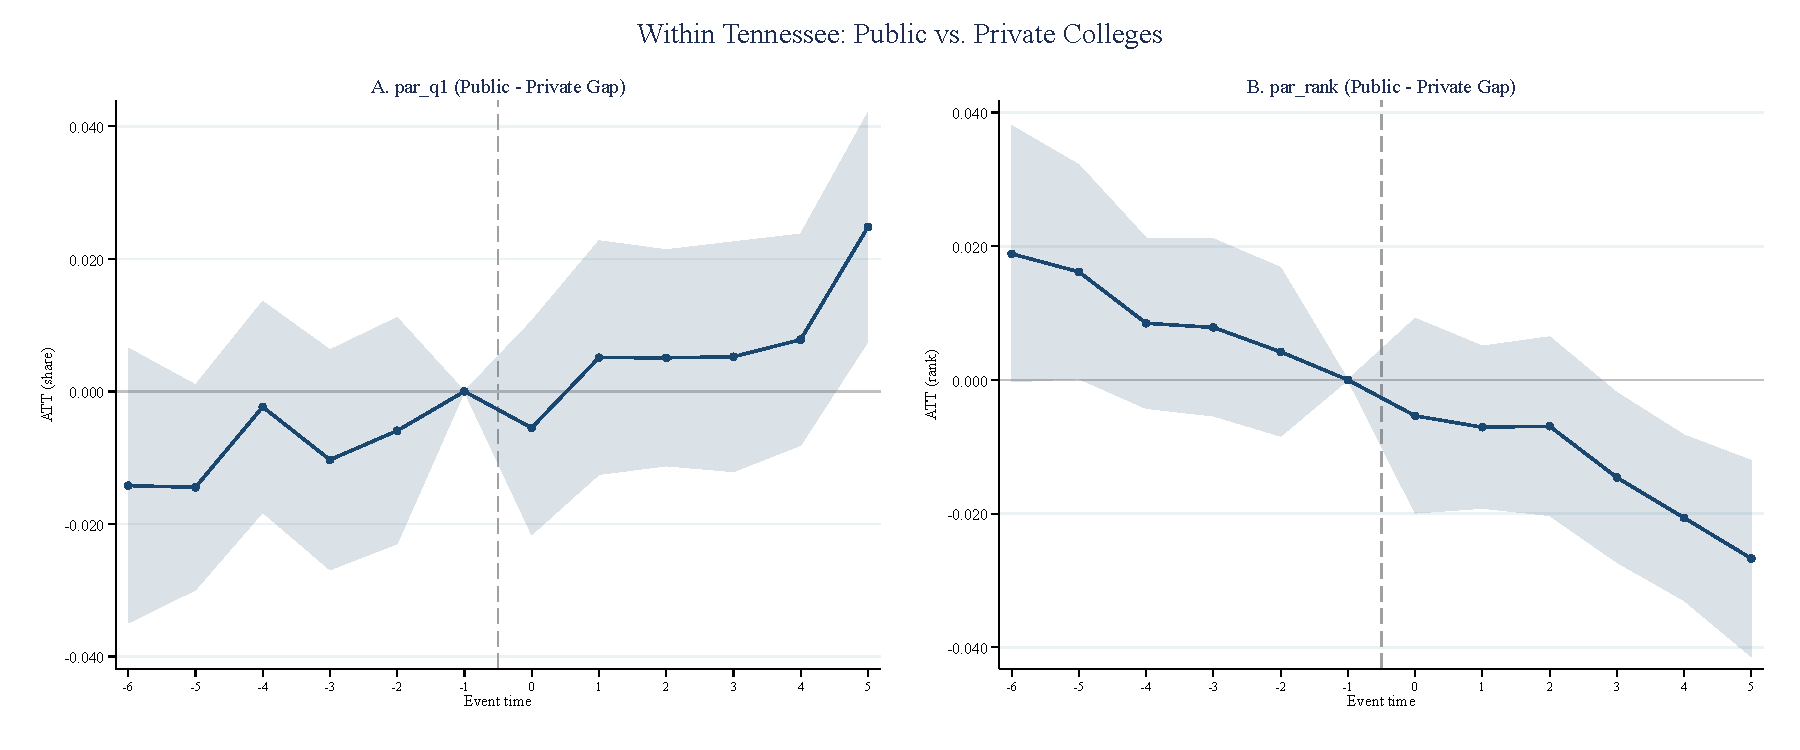
\includegraphics[width=0.9\textwidth]{fig_within_tn_comparison.pdf}
  \caption{Within-Tennessee Comparison: Public vs.\ Private Colleges}
  \label{fig:within_tn}
  \vspace{1mm}
  \begin{minipage}{0.9\textwidth}
    \footnotesize
    \textit{Notes:} Event-study estimates restricting the sample to
    Tennessee institutions only. Public colleges (treated) are compared
    to Tennessee private colleges (control). The composition shift is
    concentrated in the public sector. College and cohort fixed effects
    included. $N = 571$. Data: \textcite{chetty2020mobility}.
  \end{minipage}
\end{figure}

% Note: Estimator comparisons (LP-DiD, TWFE, Sun-Abraham, dCDH) are now
% consolidated in the four-estimator overlay figure (Figure~\ref{fig:four_estimators})
% in Section~\ref{sec:robustness_estimators}. Individual TWFE event studies
% removed to avoid redundancy.

% ============================================================
%  G. SENSITIVITY ANALYSIS
% ============================================================

% Note: R&R sensitivity is now presented as a 2×2 panel figure
% (fig_rr_combined) inline in Section 7 (Robustness). The old
% breakdown-by-event-time figure has been removed; the combined
% figure provides a cleaner summary.

% ============================================================
%  H. SPATIAL HETEROGENEITY
% ============================================================

\begin{figure}[H]
  \centering
  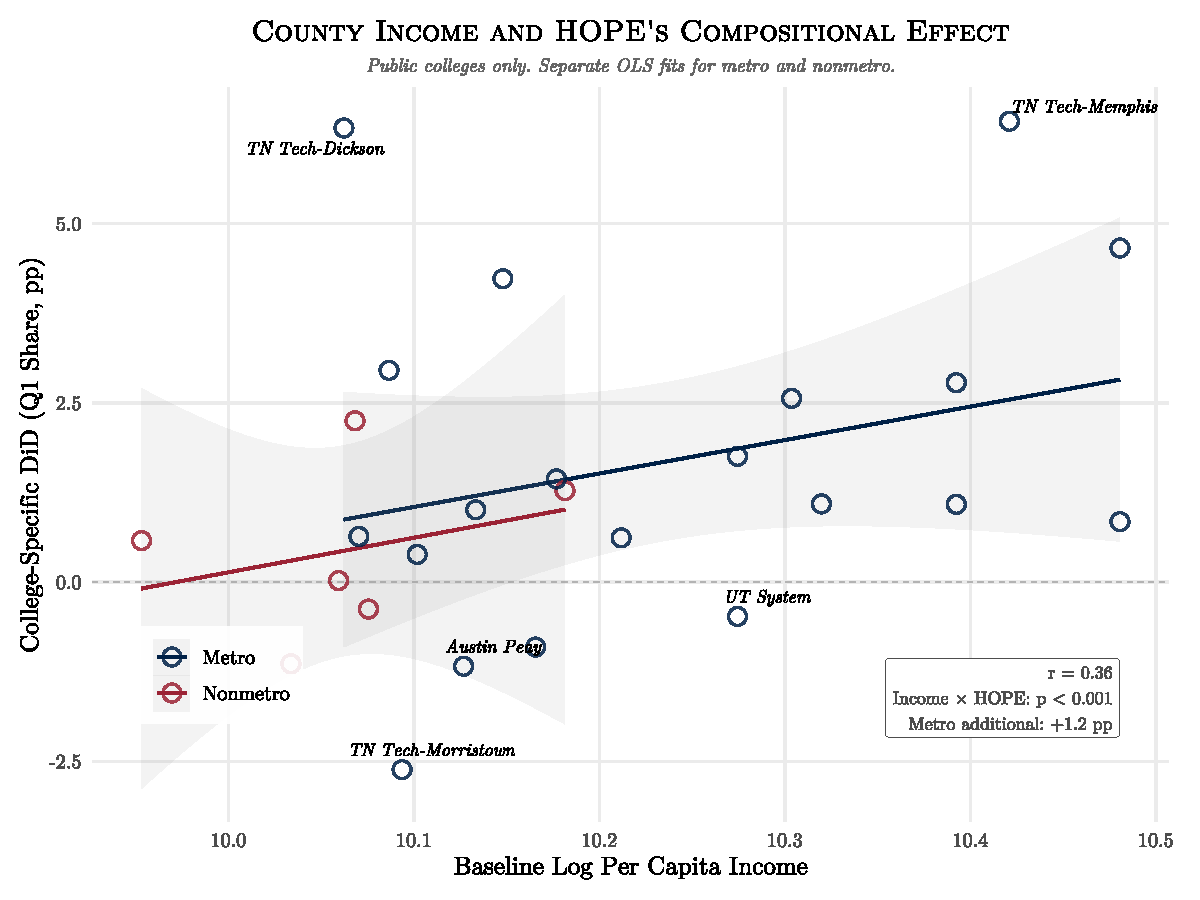
\includegraphics[width=0.9\textwidth]{fig_spatial_scatter.pdf}
  \caption{College-Level DiD Effects vs.\ Baseline County Income}
  \label{fig:spatial_scatter}
  \vspace{1mm}
  \begin{minipage}{0.9\textwidth}
    \footnotesize
    \textit{Notes:} Each point represents a Tennessee public college.
    The horizontal axis is baseline log per capita income (BEA county
    average, 1998--2003); the vertical axis is the college-specific
    TWFE DiD estimate for bottom-quintile share. Separate OLS fitted
    lines and 95\% confidence bands are shown for metro (navy) and
    nonmetro (cranberry) colleges. The overall correlation is
    $r = 0.36$; richer counties host colleges with larger progressive
    effects. Data: \textcite{chetty2020mobility}; BEA CAINC1.
  \end{minipage}
\end{figure}

\begin{figure}[H]
  \centering
  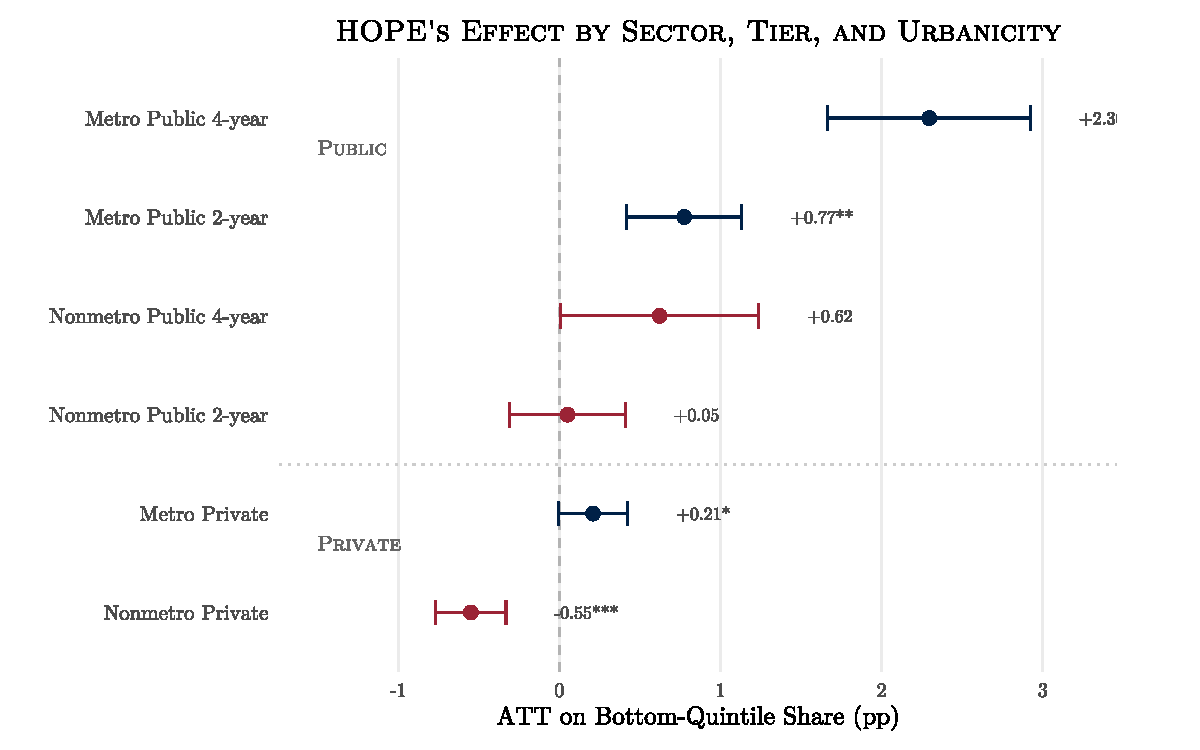
\includegraphics[width=0.9\textwidth]{fig_subgroup_forest.pdf}
  \caption{Subgroup ATT Estimates: Metro/Nonmetro $\times$ Sector and Tier}
  \label{fig:subgroup_forest}
  \vspace{1mm}
  \begin{minipage}{0.9\textwidth}
    \footnotesize
    \textit{Notes:} TWFE static DiD estimates for bottom-quintile share,
    estimated separately by metro status, sector, and tier. Metro public
    colleges---especially two-year institutions---drive the aggregate
    effect. Nonmetro public colleges show small, insignificant effects.
    Private colleges show an attenuated metro pattern consistent with
    HOPE's smaller private-institution subsidy. Horizontal bars are 95\%
    confidence intervals. Standard errors clustered at the state level.
    Data: \textcite{chetty2020mobility}.
  \end{minipage}
\end{figure}

\begin{figure}[H]
  \centering
  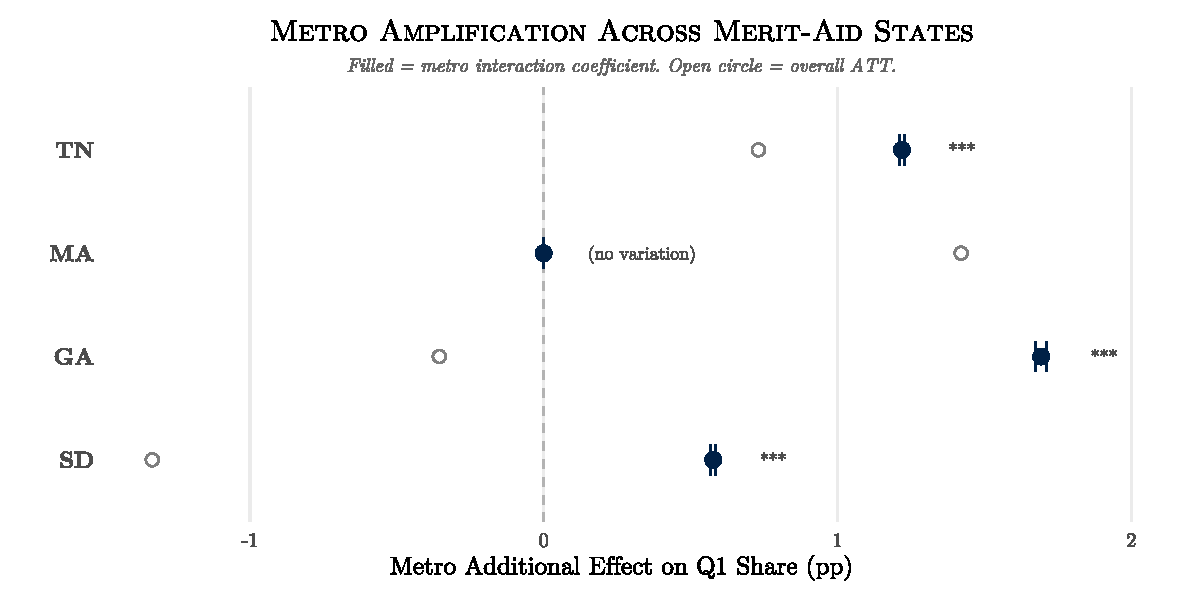
\includegraphics[width=0.9\textwidth]{fig_multistate_metro.pdf}
  \caption{Metro Interaction Coefficients Across States}
  \label{fig:multistate_metro}
  \vspace{1mm}
  \begin{minipage}{0.9\textwidth}
    \footnotesize
    \textit{Notes:} Metro $\times$ treatment interaction coefficients
    from TWFE static DiD, estimated separately for each state. Open
    circles show overall ATT for context. Tennessee, South Dakota, and
    Georgia all show positive metro interactions, indicating that the
    metro amplification is not specific to Tennessee. Massachusetts
    shows no metro variation because virtually all public colleges are
    in metro areas. Horizontal bars are 95\% confidence intervals.
    Standard errors clustered at the state level.
    Data: \textcite{chetty2020mobility}.
  \end{minipage}
\end{figure}

% ============================================================
%  I. AWARD STRUCTURE AND STATE RANKINGS
% ============================================================

\begin{figure}[H]
  \centering
  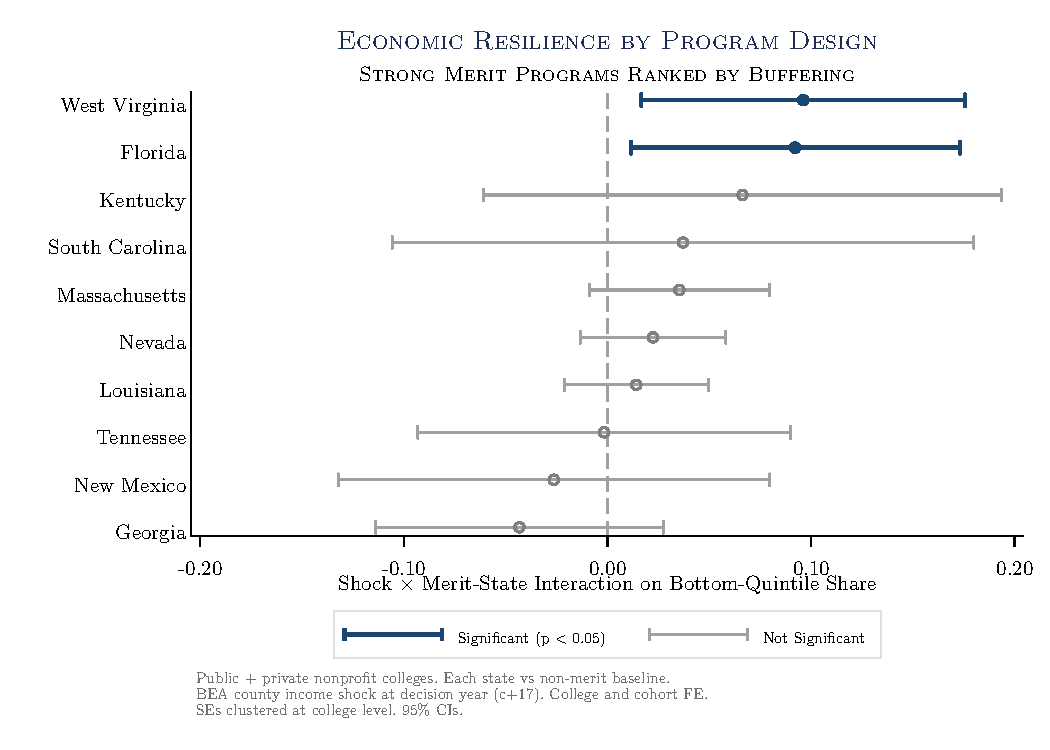
\includegraphics[width=0.85\textwidth]{fig_state_buffering.pdf}
  \caption{Economic Resilience by Program Design}
  \label{fig:state_buffering}
  \vspace{1mm}
  \begin{minipage}{0.85\textwidth}
    \footnotesize
    \textit{Notes:} Shock $\times$ merit-state interaction coefficient on
    bottom-quintile share for each strong merit program (Sjoquist \&
    Winters, 2015, plus Massachusetts). Each state estimated separately
    against non-merit baseline. Public and private nonprofit colleges.
    BEA county income shock at decision year (cohort~$+$~17). College
    and cohort FE, college-clustered SEs. 95\% CIs.
  \end{minipage}
\end{figure}

% ============================================================
%  APPENDIX B: TABLES
% ============================================================

\section{Tables}
\label{sec:tables}

% ---- Table A.1: HOPE Distribution ----
\begin{table}[H]
\centering
\begin{threeparttable}
\caption{Distribution of HOPE Scholarship Recipients by Sector, Fall 2004--2008}
\label{tab:hope_distribution}
\begin{tabular}{lccccc}
\toprule
 & 2004 & 2005 & 2006 & 2007 & 2008 \\
\midrule
\multicolumn{6}{l}{\textit{Panel A: Number of Recipients}} \\[4pt]
\quad TBR Universities         & 7,454  & 7,054  & 7,637  & 7,956  & 8,121  \\
\quad TBR Community Colleges   & 4,506  & 3,909  & 4,720  & 4,996  & 4,970  \\
\quad UT Campuses              & 5,380  & 5,310  & 5,576  & 5,988  & 6,327  \\
\quad Private Colleges         & 3,109  & 3,387  & 3,492  & 3,885  & 3,902  \\
\midrule
\textbf{Total}                 & \textbf{20,449} & \textbf{19,660} & \textbf{21,425} & \textbf{22,825} & \textbf{23,320} \\
\midrule
\multicolumn{6}{l}{\textit{Panel B: Share of Recipients (\%)}} \\[4pt]
\quad TBR Universities         & 36   & 36   & 36   & 35   & 35   \\
\quad TBR Community Colleges   & 22   & 20   & 22   & 22   & 21   \\
\quad UT Campuses              & 26   & 27   & 26   & 26   & 27   \\
\quad Private Colleges         & 15   & 17   & 16   & 17   & 17   \\
\bottomrule
\end{tabular}
\begin{tablenotes}[flushleft]
\footnotesize
\item \textit{Notes:} First-time freshmen receiving Tennessee HOPE
  Scholarship awards. TBR = Tennessee Board of Regents; UT = University
  of Tennessee system. Panel B shares may not sum to 100 due to
  rounding. Public institutions (TBR + UT) account for 83--85\% of
  recipients in all years. Source: Tennessee Student Assistance
  Corporation \parencite{THEC2025}.
\end{tablenotes}
\end{threeparttable}
\end{table}


% ---- Table A.2: Pre/Post DiD ----
\begin{table}[H]
\centering
\begin{threeparttable}
\caption{Difference-in-Differences: Pre- and Post-Treatment Means}
\label{tab:did_main}
\begin{tabular}{lcc}
\toprule
 & \textbf{Treated} & \textbf{Control} \\
 & (TN Public) & (Non-Merit States) \\
\midrule
\multicolumn{3}{l}{\textit{Panel A: Pre-Treatment Means}} \\[4pt]
\quad Bottom-quintile share & 0.138 & 0.120 \\[6pt]
\multicolumn{3}{l}{\textit{Panel B: Post-Treatment Means}} \\[4pt]
\quad Bottom-quintile share & 0.159 & 0.129 \\
\midrule
\multicolumn{3}{l}{\textit{Panel C: DiD Estimate}} \\[4pt]
\quad Treated $\times$ Post & \multicolumn{2}{c}{$0.0148^{***}$} \\
                            & \multicolumn{2}{c}{(0.0016)} \\
\midrule
College FE       & \multicolumn{2}{c}{\checkmark} \\
Cohort FE        & \multicolumn{2}{c}{\checkmark} \\
Observations     & \multicolumn{2}{c}{23,395} \\
$R^{2}$          & \multicolumn{2}{c}{0.948} \\
Clusters         & \multicolumn{2}{c}{27} \\
\bottomrule
\end{tabular}
\begin{tablenotes}[flushleft]
\footnotesize
\item \textit{Notes:} Standard errors clustered at the state level in
  parentheses. Treated = Tennessee public colleges. Control = public
  colleges in 26 states without broad-based merit programs
  \parencite{sjoquist2015state}. Post = birth cohorts 1985 and later.
  $^{***}p<0.01$, $^{**}p<0.05$, $^{*}p<0.10$.
  Data: \textcite{chetty2020mobility}.
\end{tablenotes}
\end{threeparttable}
\end{table}


% ---- Table A.3: C&S Main ATT ----
\begin{table}[H]
\centering
\begin{threeparttable}
\caption{Callaway--Sant'Anna Aggregate ATT Estimates}
\label{tab:cs_main}
\begin{tabular}{lcc}
\toprule
 & (1) & (2) \\
 & Bottom-Quintile Share & Parental Income Rank \\
\midrule
ATT & $0.0127^{***}$ & $-0.0133^{***}$ \\
    & $(0.0026)$ & $(0.0020)$ \\
\addlinespace
95\% CI & $[0.0075,\; 0.0179]$ & $[-0.0172,\; -0.0094]$ \\
\bottomrule
\end{tabular}
\begin{tablenotes}[flushleft]
\footnotesize
\item \textit{Notes:} Aggregate average treatment effect on the treated
  from \textcite{callaway2021difference}. The comparison group consists
  of never-treated public colleges in 26 non-merit-program states.
  Treatment onset: $t^* = 1986$. Analytical standard errors in
  parentheses. $^{***}p<0.01$, $^{**}p<0.05$, $^{*}p<0.10$.
  Data: \textcite{chetty2020mobility}.
\end{tablenotes}
\end{threeparttable}
\end{table}

% ---- Table A.4: TWFE Static DiD ----
\begin{table}[H]
\centering
\begin{threeparttable}
\caption{Static TWFE Difference-in-Differences Estimates}
\label{tab:twfe_did}
\begin{tabular}{lcc}
\toprule
 & (1) & (2) \\
 & Bottom-Quintile Share & Parental Income Rank \\
\midrule
TN Public $\times$ Post & $0.0142^{***}$ & $-0.0148^{***}$ \\
                         & (0.0029) & (0.0022) \\
\addlinespace
BEA Baseline Log Income  & Yes & Yes \\
College FE               & Yes & Yes \\
Cohort FE                & Yes & Yes \\
\midrule
Observations             & 5,630 & 5,630 \\
Clusters                 & 27 & 27 \\
\bottomrule
\end{tabular}
\begin{tablenotes}[flushleft]
\footnotesize
\item \textit{Notes:} Two-way fixed effects estimates with college and
  cohort fixed effects. Preferred specification: $t^* = 1987$, drop
  1980 cohort, BEA baseline county log per capita income control
  (pre-treatment average, 1997--2003). Standard errors clustered at the
  state level in parentheses. Treated = Tennessee public colleges vs.\
  public colleges in 26 non-merit states (Massachusetts excluded from
  controls). $^{***}p<0.01$, $^{**}p<0.05$, $^{*}p<0.10$.
  Data: \textcite{chetty2020mobility}.
\end{tablenotes}
\end{threeparttable}
\end{table}


% ---- Table A.5: Quintile Decomposition ----
\begin{table}[H]
\centering
\begin{threeparttable}
\caption{Quintile Decomposition: TWFE Static DiD by Income Quintile}
\label{tab:quintile_decomp}
\begin{tabular}{lccccc}
\toprule
 & (1) & (2) & (3) & (4) & (5) \\
 & Q1 (Bottom) & Q2 & Q3 & Q4 & Q5 (Top) \\
\midrule
TN Public $\times$ Post & $0.0154^{***}$ & $0.0114^{***}$ & $0.0047^{*}$ & $-0.0136^{***}$ & $-0.0179^{***}$ \\
 & $(0.0030)$ & $(0.0025)$ & $(0.0018)$ & $(0.0021)$ & $(0.0025)$ \\
\addlinespace
Observations & 6,289 & 6,289 & 6,289 & 6,289 & 6,289 \\
\bottomrule
\end{tabular}
\begin{tablenotes}[flushleft]
\footnotesize
\item \textit{Notes:} Each column reports the TWFE static
  difference-in-differences estimate from a separate regression in which
  the dependent variable is the share of students from the indicated
  income quintile. College and cohort fixed effects included. Standard
  errors clustered at the state level in parentheses (27 clusters).
  Quintile shares sum to one by construction. Post = birth cohort
  $\geq$ 1986. $^{***}p<0.01$, $^{**}p<0.05$, $^{*}p<0.10$.
  Data: \textcite{chetty2020mobility}.
\end{tablenotes}
\end{threeparttable}
\end{table}

% ---- Table A.6: Level Decomposition ----
\begin{table}[H]
\centering
\begin{threeparttable}
\caption{Level Decomposition: Share and Count Outcomes}
\label{tab:level_decomp}
\begin{tabular}{lccccc}
\toprule
 & (1) & (2) & (3) & (4) & (5) \\
 & Q1 Share & Q1 Count & Total Count & Q5 Share & Q5 Count \\
\midrule
TN Public $\times$ Post & $0.0154^{***}$ & $11.23^{**}$ & $-2.11$ & $-0.0179^{***}$ & $-34.38^{***}$ \\
                         & (0.0030) & (4.256) & (25.42) & (0.0025) & (8.635) \\
\addlinespace
Constant                 & $0.138^{***}$ & $167.9^{***}$ & $1{,}586^{***}$ & $0.200^{***}$ & $449.7^{***}$ \\
                         & (0.0001) & (0.104) & (0.622) & (0.0001) & (0.211) \\
\midrule
Observations             & 6,289 & 6,289 & 6,289 & 6,289 & 6,289 \\
Adjusted $R^{2}$         & 0.935 & 0.948 & 0.985 & 0.978 & 0.989 \\
Clusters                 & 27 & 27 & 27 & 27 & 27 \\
\bottomrule
\end{tabular}
\begin{tablenotes}[flushleft]
\footnotesize
\item \textit{Notes:} Two-way fixed effects estimates with college and
  cohort fixed effects. Standard errors clustered at the state level in
  parentheses. Count outcomes are constructed as quintile
  share $\times$ cohort size. The Q1 share increase (column 1) is
  accompanied by a Q1 count increase (column 2), while total enrollment
  is unchanged (column 3), confirming that share changes reflect
  compositional sorting rather than a denominator artifact. Post = birth
  cohort $\geq$ 1986. $^{***}p<0.01$, $^{**}p<0.05$, $^{*}p<0.10$.
  Data: \textcite{chetty2020mobility}.
\end{tablenotes}
\end{threeparttable}
\end{table}


% ---- Table A.7: Tier Heterogeneity ----
\begin{table}[H]
\centering
\begin{threeparttable}
\caption{Heterogeneity by Institution Tier: Two-Year vs.\ Four-Year Colleges}
\label{tab:tier_het}
\begin{tabular}{lcccccc}
\toprule
 & \multicolumn{3}{c}{Two-Year} & \multicolumn{3}{c}{Four-Year} \\
\cmidrule(lr){2-4} \cmidrule(lr){5-7}
Outcome & Coef. & SE & $N$ & Coef. & SE & $N$ \\
\midrule
Bottom-quintile share & $0.0181^{***}$ & $(0.0034)$ & 4,016 & $0.0070^{**}$ & $(0.0024)$ & 2,259 \\
Parental income rank & $-0.0173^{***}$ & $(0.0028)$ & 4,016 & $-0.0186^{***}$ & $(0.0021)$ & 2,259 \\
\addlinespace
Q1 count & $5.73$ & $(5.56)$ & 4,016 & $19.60^{**}$ & $(5.53)$ & 2,259 \\
Q5 count & $-22.94^{**}$ & $(6.24)$ & 4,016 & $-39.23^{*}$ & $(17.55)$ & 2,259 \\
Total count & $-58.41$ & $(35.54)$ & 4,016 & $138.52^{***}$ & $(34.66)$ & 2,259 \\
\bottomrule
\end{tabular}
\begin{tablenotes}[flushleft]
\footnotesize
\item \textit{Notes:} TWFE static difference-in-differences estimates
  estimated separately for two-year (community colleges) and four-year
  institutions. College and cohort fixed effects included. Standard
  errors clustered at the state level in parentheses. Two-year colleges
  show displacement (composition shifts, enrollment unchanged);
  four-year colleges show expansion (enrollment grows, composition
  shifts). Post = birth cohort $\geq$ 1986. $^{***}p<0.01$,
  $^{**}p<0.05$, $^{*}p<0.10$. Data: \textcite{chetty2020mobility}.
\end{tablenotes}
\end{threeparttable}
\end{table}

% ---- Table A.8: Spillover ----
\begin{table}[H]
\centering
\begin{threeparttable}
\caption{Spillover Test: Tennessee Private Colleges}
\label{tab:spillover}
\begin{tabular}{lcccc}
\toprule
Outcome & Coef. & SE & $p$-value & $N$ \\
\midrule
Bottom-quintile share & $0.0011$ & $(0.0011)$ & $0.305$ & 5,336 \\
Parental income rank & $-0.0046^{*}$ & $(0.0018)$ & $0.016$ & 5,336 \\
\bottomrule
\end{tabular}
\begin{tablenotes}[flushleft]
\footnotesize
\item \textit{Notes:} \textcite{callaway2021difference} aggregate ATT
  comparing Tennessee private colleges to private colleges in 26
  non-merit-program control states. The null effect on bottom-quintile
  share indicates that top-quintile students exiting Tennessee public
  colleges do not re-sort to in-state private institutions. Analytical
  standard errors in parentheses. $^{***}p<0.01$, $^{**}p<0.05$,
  $^{*}p<0.10$. Data: \textcite{chetty2020mobility}.
\end{tablenotes}
\end{threeparttable}
\end{table}

% ---- Table A.9: Within-TN ----
\begin{table}[H]
\centering
\begin{threeparttable}
\caption{Within-Tennessee Comparison: Public vs.\ Private Colleges}
\label{tab:within_tn}
\begin{tabular}{lcccc}
\toprule
Outcome & Coef. & SE & $p$-value & $N$ \\
\midrule
Bottom-quintile share & $0.0142^{***}$ & $(0.0037)$ & $<0.001$ & 571 \\
Parental income rank & $-0.0214^{***}$ & $(0.0032)$ & $<0.001$ & 571 \\
\bottomrule
\end{tabular}
\begin{tablenotes}[flushleft]
\footnotesize
\item \textit{Notes:} TWFE static difference-in-differences restricted
  to Tennessee institutions only. Treated = Tennessee public colleges;
  control = Tennessee private colleges. College and cohort fixed effects
  included. Standard errors in parentheses. The small sample reflects
  the within-state restriction ($N = 571$). Post = birth cohort
  $\geq$ 1986. $^{***}p<0.01$, $^{**}p<0.05$, $^{*}p<0.10$.
  Data: \textcite{chetty2020mobility}.
\end{tablenotes}
\end{threeparttable}
\end{table}

% ---- Table A.10: Robustness Summary ----
\begin{table}[H]
\centering
\begin{threeparttable}
\caption{Robustness Summary Across Estimators, Timing, and Control Groups}
\label{tab:robustness_summary}
\begin{tabular}{llcccc}
\toprule
 & & \multicolumn{2}{c}{Bottom-Quintile Share} & \multicolumn{2}{c}{Parental Income Rank} \\
\cmidrule(lr){3-4} \cmidrule(lr){5-6}
 & Specification & Coef. & SE & Coef. & SE \\
\midrule
\multicolumn{6}{l}{\textit{Panel A: Estimator}} \\
 & C\&S (preferred) & $0.0127^{***}$ & $(0.0026)$ & $-0.0133^{***}$ & $(0.0020)$ \\
 & TWFE static & $0.0154^{***}$ & $(0.0030)$ & $-0.0185^{***}$ & $(0.0025)$ \\
\addlinespace
\multicolumn{6}{l}{\textit{Panel B: Treatment Timing}} \\
 & $t^* = 1985$ & $0.0144^{***}$ & $(0.0028)$ & $-0.0180^{***}$ & $(0.0024)$ \\
 & $t^* = 1986$ (preferred) & $0.0154^{***}$ & $(0.0030)$ & $-0.0185^{***}$ & $(0.0025)$ \\
 & $t^* = 1987$ & $0.0164^{***}$ & $(0.0031)$ & $-0.0178^{***}$ & $(0.0025)$ \\
\addlinespace
\multicolumn{6}{l}{\textit{Panel C: Control Group}} \\
 & Baseline (26 states) & $0.0154^{***}$ & $(0.0030)$ & $-0.0185^{***}$ & $(0.0025)$ \\
 & Conservative & $0.0151^{***}$ & $(0.0032)$ & $-0.0175^{***}$ & $(0.0024)$ \\
 & Bordering (preferred) & $0.0144^{***}$ & $(0.0034)$ & $-0.0134^{**}$ & $(0.0049)$ \\
\addlinespace
\multicolumn{6}{l}{\textit{Panel D: Sensitivity}} \\
 & $\Delta_\text{RM}$: breakdown $\bar{M}$ & \multicolumn{2}{c}{2} & \multicolumn{2}{c}{2} \\
 & $\Delta_\text{SD}$: includes zero at & \multicolumn{2}{c}{moderate $\bar{M}$} & \multicolumn{2}{c}{moderate $\bar{M}$} \\
\bottomrule
\end{tabular}
\begin{tablenotes}[flushleft]
\footnotesize
\item \textit{Notes:} Panels A--C report static
  difference-in-differences estimates under alternative specifications.
  All specifications include college and cohort fixed effects. Standard
  errors clustered at the state level in parentheses. Panel D
  summarizes \textcite{rambachan2023more} sensitivity results: the
  $\Delta_\text{RM}$ breakdown value indicates the maximum $\bar{M}$
  at which the confidence interval excludes zero; the
  $\Delta_\text{SD}$ row indicates that confidence intervals include
  zero at moderate values of $\bar{M}$. $^{***}p<0.01$, $^{**}p<0.05$,
  $^{*}p<0.10$. Data: \textcite{chetty2020mobility}.
\end{tablenotes}
\end{threeparttable}
\end{table}


\end{document}
